\documentclass[11pt, oneside]{book}
%\documentclass[11pt, twoside]{book}  %importante cambiar si es libro
\usepackage[utf8]{inputenc}
\usepackage[T1]{fontenc}
\usepackage{times}

%%%%%%%%%%%%%%%%%%%%%%%%%%%%%%%%%%%%%%%%%%%%%%%%%%%%%%%%%
%   Paquetes y librerías iniciales para un documento,
%           Graficos, simbolos, tablas, bibliografía
%%%%%%%%%%%%%%%%%%%%%%%%%%%%%%%%%%%%%%%%%%%%%%%%%%%%%%%%%
%---------------------------------------------------------------------------
% Esto es para que el LaTeX sepa que el texto está en español:
\usepackage[spanish,es-noshorthands,es-tabla]{babel}
\selectlanguage{spanish}
%---------------------------------------------------------------------------
% para uso en modo matemático
\usepackage{amssymb}
\usepackage{amsthm}
\usepackage{amsmath}

%---------------------------------------------------------------------------
% Para las imagenes

\usepackage[dvips]{graphicx}
\graphicspath{{Figuras/}} % se fija el camino para las figuras
\usepackage{rotating}  %para poder rotar las figuras
\usepackage{wrapfig}

%---------------------------------------------------------------------------
% PIES DE FOTOS Y TABLAS

\usepackage{float} % para objetos flotantes
\usepackage{caption} % para los pies de fotos o tablas
\usepackage{subcaption}
\captionsetup{font=small,labelfont=bf} % para tamaño y tipo fuentes pie de foto
\usepackage{multirow} % para las tablas unir columnas
\usepackage{multicol} %para escribir en multiples columnas

% Referencias y biblio

\usepackage{pdfpages}
%\usepackage[pdftex,breaklinks=true,hidelinks]{hyperref} % para referencias/indice en pdf

\usepackage[
breaklinks=true,colorlinks=true,
linkcolor=blue,urlcolor=blue,citecolor=blue,% PDF VIEW
linkcolor=black,urlcolor=black,citecolor=black,% PRINT
bookmarks=true,bookmarksopenlevel=2]{hyperref}

\usepackage{emptypage}
\usepackage{ragged2e} %Justificacion

%\usepackage[toc,title,page]{appendix}

%Para bibliografía
\usepackage[numbers,square]{natbib}
%\bibliographystyle{apalike}
\bibliographystyle{IEEEtran}

%%%%%%%%% HAbituales estilos
%plainnat
%%abbrvnat
%unsrtnat  %Items in bibliography sorted in order cited)
%IEEEtran

%

%%%%%%%%%%%%%%%%%%%% Formato de la ual %%%%%%%%%%%%%%%%%%%%%%%%%%%%%%%%%


\usepackage{UAL}
%\usepackage[print,doble]{UAL}
\usepackage{codigo}

%%%%%% PAQUETES INCORPORADOS POR EL USUARIO
\usepackage{fancyvrb}
\usepackage{pdflscape}
\usepackage{geometry}
\usepackage{graphicx}
\usepackage{longtable}   %Tablas largas
\usepackage{array}
\usepackage{tabularx}
\usepackage{verbatim}
\usepackage{textcomp} %para completar los signos válidos
\usepackage{eurosym} %simbolo del euro [\euro]
\usepackage[bottom]{footmisc}
\usepackage{tikz}
\usepackage{setspace}
\usepackage[dvipsnames]{xcolor}
\definecolor{rojoPuro}{RGB}{255, 0, 0}
\newcommand{\nuevo}[1]{\textcolor{rojoPuro}{#1}}
\newcommand{\cambiado}[1]{\textcolor{blue!70!black}{#1}}
\usetikzlibrary{shapes,arrows}
\setstretch{1.15}


%%%%%%%%%%%%%%%%%%%%%%%%%%%%%%%%%%%%%%%%%%%%%%%%%%%
% Datos identificativos del TFG                            %
%%%%%%%%%%%%%%%%%%%%%%%%%%%%%%%%%%%%%%%%%%%%%%%%%%%

\author{José Luis Garrido Castro}
\titulo{Definición y desarrollo de Solución Informática para el aprendizaje del lenguaje musical}
\subTitulo{DEPARTAMENTO DE
INFORMÁTICA\\  ÁREA DE LENGUAJES Y SISTEMAS INFORMÁTICOS}
\estudios{Grado en Informática}
\universidad{UNIVERSIDAD DE ALMERÍA}
\director{Javier Criado Rodríguez}
\curso {2025/2026} 

\pagestyle{cab}
\begin{document}
 
\frontmatter

\portada

\begin{dedicatoria}
    \chapter*{Agradecimientos}
Me gustaría dar las gracias, en primer lugar, a la Escuela de Música de Huércal de Almería, al Real Conservatorio Profesional de Música de Almería y la Escuela de Música Manuel Sánchez Alonso de Canjáyar por formarme durante mis 17 últimos años, poner en mi vida este maravilloso arte que es la música y por prestarme su valiosa ayuda para este proyecto.

En segundo lugar, a mi familia ya que siempre me han apoyado a lo largo de toda mi vida y se que se sienten muy orgullosos de mis logros, en especial, los conseguidos a lo largo de este grado de Ingeniería Informática. Me han dado todo y no me cabe duda que siempre me lo darán.

Después, cabe mencionar a mis amigos que siempre estaban ahí para animarme en momentos malos y sacarme de casa cuando me hacía falta. 

En particular, quería destacar a mi compañero Jesús, con el cual llevo coincidiendo desde el instituto, manteniendo una estrecha amistad que se ha fortalecido durante el grado pasando grandes momentos y ayudándonos de forma recíproca en lo que hemos necesitado cada uno.

A mi pareja que hasta hoy no ha quedado día que no me haya preguntado como me iba con todos mis proyectos (como este) y que siempre consigue mandarme un empujón y sacarme una sonrisa para seguir llevando todo a cabo.

Por último, a todos los profesores que me han ayudado a lo largo de todo el grado y que me han transmitido todos los conocimientos posibles así como permitirme desarrollar la gran cantidad de nuevas habilidades que he conseguido durante estos años.
\end{dedicatoria}



%%%%%%%%%%%%%%%%%%%%%%%%%%%%%%%%%%%%%%%%%%%%%%%%%%%%%%%%%%%%%%%%%%%%%%%%%%%%
%%%%%%%%%%%%%%% ESTO ES PARA LA TABLA DE CONTENIDOS (INDICE)%%%%%%%%%%%%%%%%

\rmfamily
\setcounter{secnumdepth}{3} %niveles en capitulos hasta (1.1.1)
\setcounter{tocdepth}{3} %niveles en indice hasta (1.1)


\addtocontents{toc}{~\hfill\small{Página}\par} %añade "pagina" a tabla de contanidos
\addtocontents{toc}{\vspace{2pt} \hrule \vspace{5mm} \par}

%\renewcommand\contentsname{Índice de contenidos}
\tableofcontents
\listoffigures % indice de figuras
\listoftables % indice de tablas



%---------------------------------------------------------------------------
% comienzo de relacion abreviaturas y/o acrónimos
%---------------------------------------------------------------------------


%\addcontentsline{toc}{section}{ABREVIATURAS}
\clearpage


%\addcontentsline{toc}{section}{ABREVIATURAS}




%se suelen utilizar archivos separados, por capitulos para agilizar la compilación en las versiones intermedias
\mainmatter
\marcagua

\chapter{Introducción}
\label{chap:introduccion}

\section{Introducción}

El presente trabajo constituye un \textbf{complemento y una evolución directa del Trabajo Fin de Grado} desarrollado previamente, en el que se diseñó, implementó y validó una aplicación destinada a facilitar la enseñanza y el aprendizaje del lenguaje musical mediante una plataforma web basada en una arquitectura cliente-servidor. En dicho proyecto se realizó un estudio completo de la problemática existente en este ámbito, comenzando con un marco teórico sobre la enseñanza del lenguaje musical y continuando con una investigación apoyada en encuestas y entrevistas a alumnado y profesorado. Este análisis permitió identificar las principales necesidades presentes en el proceso de enseñanza, así como las limitaciones de las herramientas digitales disponibles, sirviendo de base para la definición de los requisitos y el posterior desarrollo de una solución informática.

Como resultado de aquel trabajo se obtuvo una aplicación funcional capaz de gestionar usuarios con distintos roles, grupos de clase, materiales docentes, tareas, cuestionarios, calificaciones y un sistema de comunicación interna, todo ello apoyado por una arquitectura basada en una API REST, una interfaz híbrida desarrollada con Ionic y Angular, una base de datos MongoDB y diferentes mecanismos destinados a garantizar la seguridad, la calidad del software y la automatización del despliegue.

No obstante, tanto durante el desarrollo del proyecto como tras la validación de la aplicación se identificaron diferentes líneas de mejora que no pudieron abordarse dentro del alcance temporal del Trabajo Fin de Grado. La experiencia adquirida durante la implementación puso de manifiesto que, aunque la plataforma cumplía con los objetivos inicialmente planteados y demostraba la viabilidad de la propuesta, todavía existía un importante margen de evolución para convertirla en una herramienta más completa, robusta y preparada para ser utilizada en un contexto educativo real.

Este complemento nace precisamente con ese propósito. En lugar de desarrollar una nueva aplicación o replantear la solución existente, el trabajo parte de una base completamente funcional y centra sus esfuerzos en su evolución. Se mantiene la arquitectura, la metodología de desarrollo y las principales decisiones de diseño adoptadas durante el Trabajo Fin de Grado, aprovechando el trabajo ya realizado para ampliar las capacidades del sistema y aumentar su grado de madurez.
Por tanto, el objetivo de este complemento no consiste únicamente en incorporar nuevas funcionalidades, sino en consolidar la aplicación como un proyecto con continuidad, abordando aspectos que trascienden al propio desarrollo software y que resultan imprescindibles cuando una aplicación deja de ser un prototipo académico para acercarse a un escenario de utilización real. En este sentido, además de la evolución funcional de la plataforma, el trabajo estudia aquellos elementos técnicos, organizativos y de seguridad necesarios para facilitar una futura implantación en centros educativos, sentando así las bases para las siguientes fases de desarrollo del proyecto.

\section{La aplicación desarrollada}

La aplicación sobre la que se desarrolla este complemento mantiene la filosofía y la arquitectura definidas en el Trabajo Fin de Grado, preservando una estructura cliente-servidor basada en una API REST y un frontend híbrido desarrollado con Ionic y Angular. Esta continuidad tecnológica permite que todas las mejoras incorporadas se integren sobre una base consolidada, evitando modificaciones estructurales innecesarias y garantizando la reutilización del trabajo previamente realizado.

Desde el punto de vista funcional, el trabajo se centra, en primer lugar, en la mejora y refinamiento de las funcionalidades ya existentes. Se revisan diferentes módulos de la aplicación con el objetivo de optimizar su funcionamiento, mejorar la experiencia de usuario y adaptar determinados procesos a las necesidades detectadas durante el desarrollo inicial. Estas mejoras permiten incrementar la estabilidad del sistema, facilitar la interacción de los distintos tipos de usuarios y aumentar la coherencia general de la plataforma.

Junto a esta evolución de los módulos existentes, el proyecto incorpora nuevas funcionalidades que amplían el alcance de la aplicación y enriquecen las posibilidades que ofrece tanto al profesorado como al alumnado. Estas nuevas capacidades se integran respetando la arquitectura original y siguiendo los mismos principios de modularidad, reutilización y separación de responsabilidades empleados durante el desarrollo del proyecto base.

Una de las principales novedades introducidas en esta fase es la integración de un servicio externo de inteligencia artificial mediante la API de Groq. Esta incorporación permite que la aplicación pueda consumir servicios de inferencia basados en modelos de lenguaje sin necesidad de desplegar infraestructura propia para ello. La integración se realiza desde el backend, manteniendo completamente desacoplada la lógica de negocio del servicio de inteligencia artificial y permitiendo que dicho proveedor pueda ser sustituido en el futuro sin afectar al resto del sistema. Con ello se dota a la plataforma de nuevas posibilidades de interacción y generación de contenido, manteniendo al mismo tiempo la coherencia arquitectónica del proyecto.

Otra de las líneas de evolución más relevantes consiste en ampliar el alcance de la aplicación más allá del entorno web. Aprovechando la naturaleza híbrida del frontend desarrollado con Ionic y Angular, se incorpora Capacitor como puente entre la aplicación y el sistema operativo móvil, permitiendo generar una versión instalable para dispositivos Android sin necesidad de desarrollar una nueva aplicación nativa. Esta adaptación mantiene una única base de código para todas las plataformas, favoreciendo la mantenibilidad del proyecto y garantizando una experiencia homogénea para los usuarios.

Como complemento a esta adaptación, también se incorpora Android Studio como entorno de construcción, empaquetado, depuración y validación de la aplicación móvil. De esta manera, el proyecto no solamente demuestra la viabilidad de la plataforma en un navegador web, sino también su capacidad para ejecutarse como una aplicación instalada en dispositivos móviles, ampliando considerablemente las posibilidades de utilización en un entorno educativo.

Finalmente, todas estas mejoras se desarrollan respetando la arquitectura tecnológica existente, manteniendo el uso de MongoDB como sistema de persistencia, JWT para la autenticación y autorización de usuarios, Swagger como herramienta de documentación de la API, los distintos sistemas de pruebas automatizadas y el flujo de integración y despliegue continuo mediante GitHub Actions, Render y GitHub Pages. Gracias a ello, la evolución de la aplicación se produce de forma controlada, manteniendo la escalabilidad, la mantenibilidad y la calidad técnica alcanzadas durante el proyecto original.
\section{Estructura de la memoria}

La presente memoria se organiza en varios capítulos que describen de forma progresiva el desarrollo realizado durante este complemento del Trabajo Fin de Grado. Cada uno de ellos aborda una fase concreta del proyecto, desde la contextualización inicial hasta la valoración final de los resultados obtenidos.

\begin{itemize}

    \item \textbf{Introducción.}  
    Presenta el propósito del complemento, su relación con el Trabajo Fin de Grado original y ofrece una visión general tanto de la evolución de la aplicación como de la organización de la memoria.

    \item \textbf{Objetivos.}  
    Define el objetivo general del proyecto y los objetivos específicos que orientan esta nueva fase de desarrollo. Asimismo, se incluye la planificación seguida durante la realización del complemento, mostrando la continuidad respecto al proyecto base.

    \item \textbf{Análisis, definición y arquitectura.}  
    Constituye el núcleo técnico de la memoria. En este capítulo se analizan las necesidades abordadas durante esta fase del proyecto, se describen las mejoras realizadas sobre las funcionalidades existentes y las nuevas capacidades incorporadas a la aplicación, así como las decisiones arquitectónicas y tecnológicas adoptadas para su integración, manteniendo la coherencia con la solución desarrollada previamente.

    \item \textbf{Flujo de trabajo.}  
    Muestra el funcionamiento de la aplicación a través de los principales flujos de uso. Mediante distintos ejemplos se describe cómo interactúan los diferentes tipos de usuarios con la plataforma, ilustrando el comportamiento de las funcionalidades más relevantes y permitiendo comprender el funcionamiento global del sistema desde un punto de vista práctico.

    \item \textbf{Plan de implantación.}  
    Estudia los aspectos necesarios para facilitar una futura implantación de la aplicación en centros educativos. Se analizan cuestiones relacionadas con la infraestructura necesaria, la seguridad, la gestión de usuarios y datos, el despliegue de la plataforma, el mantenimiento y otros factores organizativos que condicionan la utilización de la aplicación en un entorno real.

    \item \textbf{Conclusiones y líneas de trabajo futuro.}  
    Recoge una valoración global del proyecto, analizando el grado de cumplimiento de los objetivos planteados y los resultados obtenidos. Finalmente, se presentan las principales líneas de evolución que permitirán continuar ampliando las capacidades de la aplicación y avanzar progresivamente hacia su implantación en entornos educativos reales.

\end{itemize}



\chapter{Contexto del proyecto y punto de partida}
\label{chap:contexto}
El desarrollo de este complemento parte de una solución previamente diseñada e implementada durante el Trabajo Fin de Grado. Dicha solución constituye el punto de partida sobre el que se construye la evolución presentada en esta memoria y proporciona tanto la base tecnológica como el análisis previo que justifican las decisiones adoptadas en esta nueva fase del proyecto.

Por este motivo, antes de describir las ampliaciones realizadas, resulta conveniente resumir los aspectos más relevantes del proyecto original que sirven de contexto para comprender la evolución desarrollada en este complemento.
\section{Marco teórico, investigación y estudio previo}
En el proyecto original se estableció, en primer lugar, un marco teórico que permitió contextualizar el lenguaje musical como disciplina educativa, analizando su papel dentro de la formación musical y las dificultades habituales asociadas a su aprendizaje y enseñanza. Este marco teórico puso de manifiesto una serie de problemáticas recurrentes, tales como la falta de recursos digitales específicos, la escasa adaptación de las herramientas existentes a las dinámicas reales del aula y la dificultad para realizar un seguimiento individualizado del alumnado en este ámbito.

A partir de esta base teórica, se llevó a cabo una investigación empírica apoyada en encuestas y entrevistas a profesores y alumnos de lenguaje musical, cuyo objetivo fue contrastar las problemáticas identificadas y detectar necesidades concretas desde la experiencia directa en entornos educativos reales. Paralelamente, se realizó un estudio basado en una revisión bibliográfica de trabajos previos y soluciones existentes, lo que permitió situar el proyecto dentro del estado del arte y analizar las limitaciones y oportunidades de las herramientas disponibles en la actualidad.

La combinación de marco teórico, investigación empírica y revisión bibliográfica proporcionó una base sólida para la definición de los requisitos funcionales y no funcionales del sistema, así como para la formulación de los objetivos del proyecto. Como resultado de este proceso, se diseñó e implementó una plataforma informática compuesta por un backend basado en una API REST y un frontend híbrido y accesible.
\section{Resultados del proyecto base y líneas de evolución}
La aplicación desarrollada en la versión inicial permite gestionar usuarios, grupos, material de clase, calificaciones, cuestionarios, tareas y comunicaciones internas, incorporando además mecanismos de autenticación, pruebas automatizadas, documentación técnica y procesos de despliegue continuo. Esta primera versión del sistema fue validada funcionalmente, demostrando su viabilidad técnica y su adecuación inicial a las necesidades detectadas.

No obstante, tanto las conclusiones del proyecto como la experiencia práctica derivada del uso de la aplicación evidenciaron que la solución implementada, aun siendo plenamente funcional, presenta margen de mejora y evolución. En particular, se identificaron oportunidades para refinar determinadas funcionalidades existentes, incorporar nuevas capacidades que amplíen el alcance de la aplicación y abordar de forma más profunda su implantación en entornos educativos reales. Estas líneas de evolución quedaron recogidas explícitamente como trabajo futuro en el proyecto original.

En este contexto, el presente proyecto no pretende repetir ni reformular el marco teórico ni los estudios ya realizados, sino apoyarse en ellos como base validada para dar un paso adicional. El foco se desplaza desde el desarrollo inicial de la solución hacia su extensión funcional y su preparación para una implantación realista y sostenible, considerando aspectos técnicos, organizativos y de seguridad que resultan fundamentales en un escenario de uso continuado.

De este modo, este trabajo se plantea como una continuación natural y coherente del proyecto previo, orientada a consolidar la solución desarrollada y a sentar las bases necesarias para su evolución e implantación efectiva en centros educativos, manteniendo la alineación con la problemática detectada y con los principios pedagógicos que motivaron el trabajo previo.
\section{Tecnologías y arquitectura de la solución extendida}
\label{sec:tecnologias_ext}

La solución extendida mantiene la arquitectura global cliente-servidor \cite{Tanenbaum2007} basada en una API REST y una organización inspirada en el patrón MVC (Modelo-Vista-Controlador) idéntica en su planteamiento a la versión inicial. Esta continuidad tecnológica no es accidental: la pila original proporciona un equilibrio adecuado entre modularidad, escalabilidad y facilidad de mantenimiento, lo que permite incorporar nuevas capacidades sin necesidad de reestructurar el sistema ni introducir deuda técnica \cite{Pressman2010}.

\subsection{Pila tecnológica heredada del proyecto base}

El proyecto se apoya en un conjunto de tecnologías consolidadas que cubren de manera eficaz las necesidades de una aplicación educativa con múltiples roles, gestión de contenidos multimedia y comunicación bidireccional:

\begin{itemize}
    \item \textbf{Ionic + Angular (Frontend).}  
    Se mantiene un frontend híbrido desarrollado con Ionic y Angular, que permite construir una interfaz responsive y reutilizable tanto en entorno web como móvil.  
    Angular aporta una estructura basada en componentes, servicios y módulos que facilita la organización del código, la reutilización de lógica y la separación entre presentación y lógica de negocio, mientras que Ionic proporciona componentes visuales optimizados para dispositivos táctiles y móviles.
\newpage
    \item \textbf{Node.js + Express (Backend).}  
    El backend continúa implementándose mediante un servidor Node.js con Express, exponiendo una API REST encargada de centralizar la lógica de negocio, la validación de datos y la aplicación de reglas de acceso.  
    Esta combinación ofrece un entorno ligero y flexible, adecuado para aplicaciones con múltiples operaciones CRUD y consumo intensivo de recursos multimedia.

    \item \textbf{MongoDB (Persistencia).}  
    Se mantiene una base de datos documental MongoDB para almacenar los datos que requieren de persistencia.  
    El modelo no relacional facilita la evolución del esquema de datos y permite representar relaciones entre entidades educativas sin penalizar la flexibilidad, algo especialmente relevante en un sistema que crece de forma incremental. También se hace uso de MongoDB Atlas, un servicio gestionado en la nube que ofrece una solución escalable y segura.

    \item \textbf{JWT (Autenticación y autorización).}  
    La autenticación se sigue gestionando mediante JSON Web Tokens, permitiendo un control claro de sesiones y permisos en función del rol del usuario.  
    Este enfoque se adapta bien a una arquitectura REST y evita mantener estado de sesión en el servidor.

    \item \textbf{Swagger / OpenAPI (Documentación).}  
    La documentación de la API se mantiene mediante Swagger, proporcionando una especificación clara y verificable de los endpoints disponibles, útil tanto para pruebas como para mantenimiento futuro.

    \item \textbf{Testing (Jest/Supertest y Jasmine/Karma).}  
    Se conserva el uso de Jest y Supertest para pruebas del backend, y Jasmine/Karma para el frontend, permitiendo validar de manera automatizada el comportamiento del sistema y reducir regresiones durante la evolución del proyecto.
    
    \item \textbf{Integración y despliegue continuo (Render, GitHub Actions y Pages).}
    Se continúa ejecutando el flujo de integración y despliegue continuo en GitHub Actions para automatizar el testing y el despliegue, que será realizado en Render para el backend y GitHub Pages para el frontend.
\end{itemize}

\subsection{Tecnologías incorporadas en la solución extendida}

La extensión del sistema introduce nuevas tecnologías que amplían las capacidades técnicas de la aplicación sin modificar su arquitectura base ni los principios de diseño definidos en el trabajo previo. Estas tecnologías se integran como componentes complementarios, manteniendo el desacoplamiento y la coherencia estructural del sistema.

\subsubsection{Servicio de inferencia externa mediante Groq}

Se incorpora un servicio de inferencia externa utilizando Groq \cite{groq_docs} como proveedor, haciendo uso de su API pública para el envío de peticiones desde el backend del sistema. En este contexto, Groq actúa como un servicio externo capaz de procesar \textit{prompts} de inteligencia artificial y devolver respuestas generadas a partir de modelos de lenguaje, sin que dichos modelos formen parte de la infraestructura propia de la aplicación.
\newpage
Desde un punto de vista tecnológico, la utilización de la API de Groq implica la integración de un servicio HTTP externo que recibe solicitudes estructuradas \cite{RFC9110}, incluyendo el contenido del \textit{prompt}, y devuelve una respuesta generada en un formato estándar (por ejemplo, JSON). Esta aproximación permite tratar el sistema de inferencia como un recurso remoto, consumido de forma análoga a cualquier otro servicio web.

El uso de una API de inferencia externa presenta varias implicaciones técnicas relevantes:
\begin{itemize}
    \item Permite externalizar el procesamiento asociado a modelos de lenguaje, evitando la necesidad de desplegar, mantener o escalar infraestructura específica para inferencia.
    \item Facilita el control del flujo de peticiones, ya que las llamadas a la API pueden regularse, validarse y encapsularse desde el backend.
    \item Aísla la lógica de generación de contenido del resto del sistema, permitiendo modificar el proveedor o el modelo utilizado sin afectar a la arquitectura interna.
\end{itemize}

Desde el punto de vista del diseño software, la integración mediante una API externa refuerza el desacoplamiento del sistema, ya que el servicio de inferencia se consume como una dependencia claramente delimitada, manteniendo la coherencia con la arquitectura por capas adoptada en el proyecto.

\begin{figure}[H]
    \centering
    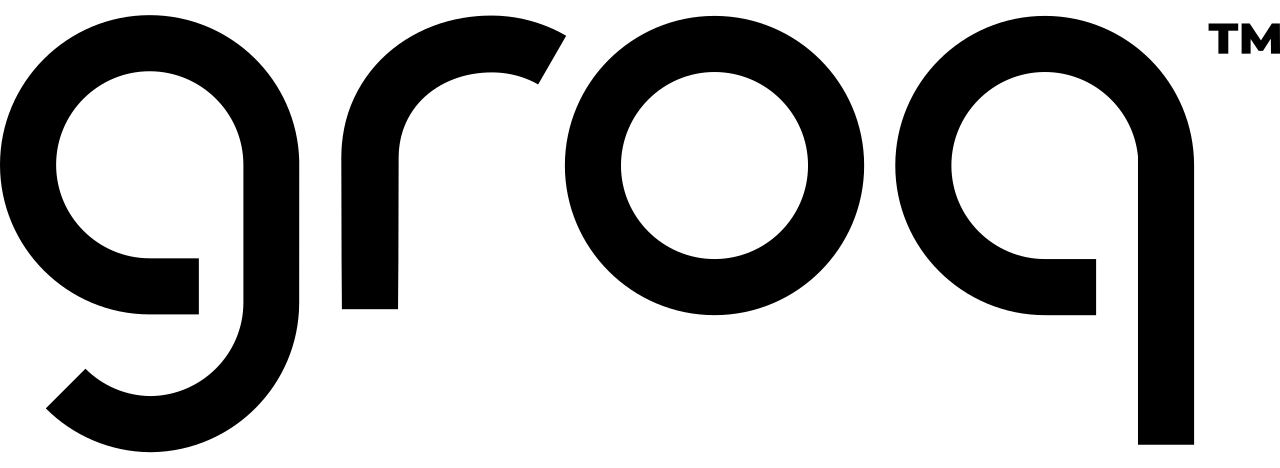
\includegraphics[height=2cm]{Figuras/logos/groq.png}
    \caption{Groq}
    \label{fig:logo_groq}
\end{figure}

\subsubsection{Capacitor como evolución del soporte móvil híbrido}

El uso de Ionic junto con Angular permite abordar el desarrollo multiplataforma mediante una única base de código. Este enfoque resuelve gran parte de los problemas asociados a la portabilidad de la interfaz y de la lógica de la aplicación, tanto en entorno web como en dispositivos móviles. No obstante, el desarrollo puramente web presenta una limitación clara: existen funcionalidades propias del sistema operativo móvil que no pueden ser gestionadas directamente desde el navegador.

\textbf{Primeros intentos de integración nativa.}  
Para cubrir esta necesidad surgió Cordova \cite{cordova_docs}, cuya función principal era actuar como un puente entre la aplicación web y el dispositivo. Gracias a esta tecnología fue posible acceder desde JavaScript a funcionalidades nativas, permitiendo que las aplicaciones híbridas pudieran comportarse como aplicaciones móviles instaladas. En su contexto histórico, Cordova supuso un avance clave para validar el modelo híbrido.

Sin embargo, Cordova respondía a una etapa temprana de esta evolución. A medida que las aplicaciones comenzaron a requerir mayor control y personalización del entorno móvil, sus limitaciones se hicieron evidentes.
\newpage
\textbf{Evolución hacia un modelo más flexible.}  
Capacitor \cite{capacitor_docs} aparece como la evolución natural de este enfoque, manteniendo la reutilización del código web, pero adaptándolo a las necesidades actuales del desarrollo móvil. La diferencia entre ambos modelos puede resumirse claramente en los siguientes puntos:

\begin{itemize}
    \item \textbf{Relación con el código nativo}: Cordova ocultaba en gran medida la capa nativa, mientras que Capacitor la integra como parte explícita del proyecto.
    \item \textbf{Configuración del sistema}: En Cordova, los ajustes específicos resultaban complejos y poco transparentes; Capacitor facilita configuraciones controladas y mantenibles.
    \item \textbf{Evolución y mantenimiento}: Capacitor se alinea mejor con las herramientas y prácticas actuales del desarrollo móvil, favoreciendo la sostenibilidad del proyecto.
\end{itemize}

\textbf{Papel actual de Capacitor en el proyecto.}  
En la actualidad, Capacitor no se limita únicamente al empaquetado de la aplicación y a su ejecución como aplicación instalada, funciones que ya desempeñaba Cordova. Su principal aportación es actuar como una capa de integración que permite extender el frontend híbrido con capacidades propias del entorno móvil cuando el proyecto lo requiere.

En el contexto de este proyecto, Capacitor resulta especialmente relevante porque:
\begin{itemize}
    \item Permite generar una aplicación móvil instalable a partir del frontend híbrido existente.
    \item Mantiene una única base de código, garantizando coherencia funcional entre la versión web y la versión móvil.
    \item Facilita la incorporación de funcionalidades y configuraciones específicas del dispositivo sin alterar la arquitectura del sistema.
\end{itemize}

De este modo, Capacitor se incorpora como un elemento habilitador que amplía el alcance de la solución, facilitando su implantación real en dispositivos móviles y manteniendo los principios de reutilización, modularidad y separación de responsabilidades definidos en el proyecto.
\begin{figure}[H]
    \centering
    
\includegraphics[height=3cm]{Figuras/logos/Capacitor.png}
    \caption{Capacitor}
    \label{fig:logo_Capacitor}
\end{figure}
\newpage
\subsubsection{Android Studio y entorno de construcción móvil}

La tercera tecnología incorporada es Android Studio \cite{android_studio_docs}, utilizado como entorno de construcción, empaquetado y validación de la aplicación en dispositivos Android. Su inclusión se apoya en el carácter híbrido del frontend, que permite reutilizar la misma base de código web para generar una aplicación instalable.

Desde el punto de vista tecnológico, el uso de Android Studio implica:
\begin{itemize}
    \item La integración con la cadena de herramientas oficial de Android para la compilación, firma y despliegue de aplicaciones.
    \item La generación de un contenedor nativo que encapsula la aplicación híbrida, permitiendo su ejecución como aplicación instalada.
    \item El acceso a herramientas de depuración, emulación y análisis propias del ecosistema Android.
\end{itemize}

Este enfoque no introduce una nueva base de código ni una bifurcación tecnológica, sino que extiende el alcance del sistema aprovechando el diseño \textit{responsive} existente. De este modo, la portabilidad se aborda como una extensión técnica natural del frontend híbrido, sin duplicar lógica ni comprometer la consistencia del sistema.

\begin{figure}[H]
    \centering
    
\includegraphics[height=3cm]{Figuras/logos/android_studio.png}
    \caption{Android Studio.}
    \label{fig:logo_android_studio}
\end{figure}

En conjunto, las tecnologías incorporadas refuerzan la arquitectura existente, ampliando las capacidades del sistema desde un punto de vista estrictamente técnico y manteniendo los principios de modularidad, reutilización y separación de responsabilidades definidos en el trabajo previo.

A nivel conceptual, la arquitectura global permanece idéntica. Se incluye a continuación, en la Figura \ref{fig:arquitectura_global_ext}, el diagrama original para facilitar la lectura del documento sin obligar a consultar constantemente la versión original.

\tikzstyle{block} = [rectangle, draw, node distance=4.5cm,
    text width=6em, text centered, rounded corners, minimum height=3em, fill=blue!10]
\tikzstyle{line} = [draw, -latex']

\begin{figure}[H]
\centering
\begin{tikzpicture}
    \node [block] (Frontend) {Frontend \\ (Ionic + Angular)};
    \node [block, below of=Frontend, node distance=5cm] (Backend) {Backend REST \\ (Node.js + Express)};
    \node [block, below of=Backend, node distance=5cm] (DB) {Base de datos \\ (MongoDB)};
    \node [block, left of=Backend, node distance=7.2cm] (External) {Servicios externos};
    \node [block, right of=Backend, node distance=6.3cm] (CI) {CI/CD \\ (GitHub Actions + Render)};
    \path [line] ([xshift=-1.5mm]Frontend.south) -- node[left] {Solicitudes API} ([xshift=-1.5mm]Backend.north);
    \path [line] ([xshift=1.5mm]Backend.north) -- node[right] {Respuestas API} ([xshift=1.5mm]Frontend.south);
    \path [line] ([xshift=-1.5mm]Backend.south) -- ([xshift=-1.5mm]DB.north);
    \path [line] ([xshift=1.5mm]DB.north) -- ([xshift=1.5mm]Backend.south);
    \path [line] (Backend.west) -- (External.east);
    \path [line] (CI) -- (Backend);
    \path [line] (CI) to[bend right=20] (Frontend);
\end{tikzpicture}
\caption{Arquitectura global de la aplicación (sin cambios respecto al proyecto base)}
\label{fig:arquitectura_global_ext}
\end{figure}

Con esta arquitectura, la solución extendida queda descrita con el mismo enfoque de la primera versión: continuidad en arquitectura y metodología, y ampliación funcional bien acotada, verificable y orientada a la implantación real.


\chapter{Objetivos del proyecto}
\label{chap:objetivos}

En este capítulo se presentan los objetivos que guían el desarrollo del presente trabajo, concebido como una ampliación y evolución de la aplicación desarrollada previamente en el Trabajo Fin de Grado. En primer lugar, se define el objetivo general, que establece la finalidad principal de esta nueva fase del proyecto. Posteriormente, se detallan los objetivos específicos cuya consecución permitirá incrementar las capacidades de la aplicación y prepararla para un escenario de utilización más próximo a un entorno educativo real.

\section{Objetivo general}

El objetivo general de este proyecto consiste en \textbf{extender y consolidar la solución informática desarrollada en el Trabajo Fin de Grado, incorporando nuevas funcionalidades, mejorando las ya existentes y preparándola para su futura implantación en centros educativos reales}.

Partiendo de una aplicación funcional desarrollada durante el proyecto inicial, esta nueva fase tiene como finalidad aumentar su grado de madurez, mejorando tanto sus prestaciones como su calidad técnica. Para ello, no solo se pretende ampliar las funcionalidades disponibles, sino también optimizar aquellas ya implementadas, adaptar la aplicación a nuevos entornos de ejecución y definir los aspectos necesarios para que pueda evolucionar desde un prototipo funcional hacia una herramienta preparada para un uso real.

Asimismo, este proyecto busca mantener la coherencia con la arquitectura y las decisiones de diseño adoptadas en el Trabajo Fin de Grado, aprovechando la base ya desarrollada para incorporar nuevas capacidades sin comprometer la mantenibilidad ni la escalabilidad de la aplicación.

\section{Objetivos específicos}

Con el fin de alcanzar el objetivo general, se han definido los siguientes objetivos específicos:

\begin{itemize}

\item \textbf{Mejorar y refinar las funcionalidades existentes de la aplicación.}

Este objetivo persigue revisar las funcionalidades implementadas durante el Trabajo Fin de Grado con el propósito de optimizar su funcionamiento, mejorar la experiencia de usuario y adaptar la aplicación a las necesidades detectadas tras el desarrollo inicial. Se pretende aumentar la usabilidad, la estabilidad y la coherencia de la interfaz, facilitando su utilización en un contexto educativo.
\newpage
\item \textbf{Diseñar e incorporar nuevas funcionalidades innovadoras.}

La ampliación de la aplicación requiere el desarrollo de nuevos módulos y herramientas que complementen las capacidades existentes y aporten un valor añadido respecto a la versión inicial. Estas nuevas funcionalidades estarán orientadas a enriquecer la experiencia de aprendizaje, ampliar las posibilidades de interacción y responder a necesidades que no pudieron abordarse durante el desarrollo del proyecto base.

\item \textbf{Facilitar el despliegue de la aplicación en dispositivos móviles aprovechando su arquitectura híbrida.}

Se pretende adaptar la aplicación para que pueda ejecutarse de forma nativa en dispositivos Android utilizando la misma base de código desarrollada para la versión web. Para ello, se aprovechará el diseño responsive y las tecnologías híbridas empleadas, garantizando una experiencia de usuario homogénea y optimizada en distintos tamaños de pantalla y favoreciendo el acceso a la plataforma desde cualquier dispositivo.

\item \textbf{Definir un plan de implantación orientado a centros educativos reales.}

Además del desarrollo técnico, resulta necesario establecer las bases que permitan una futura implantación de la aplicación en un entorno educativo. Este objetivo contempla el estudio de los requisitos tecnológicos necesarios, la mejora de aspectos relacionados con la seguridad, la gestión de archivos y datos, la administración de usuarios y la planificación del despliegue, con el propósito de evaluar la viabilidad de la solución en escenarios reales.

\end{itemize}

La consecución de estos objetivos permitirá evolucionar la aplicación desarrollada en el Trabajo Fin de Grado hacia una solución más completa, robusta y preparada para afrontar futuras fases de implantación, manteniendo la continuidad del proyecto original y ampliando significativamente sus capacidades.
\section{Planificación del proyecto}
\label{chap:planificacion}

La planificación de este proyecto de complemento se concibe como una continuación directa de la planificación establecida en el proyecto original, manteniendo sus mismos principios de organización, seguimiento y control temporal. Dado que la arquitectura base y las funcionalidades nucleares del sistema ya se encontraban definidas e implementadas, no ha sido necesario replantear el cronograma global, sino ampliarlo de forma coherente para dar cabida a las nuevas tareas derivadas de la evolución funcional, tecnológica y operativa de la solución.

En este contexto, la planificación se ha centrado específicamente en estructurar y calendarizar las actividades asociadas a la mejora de funcionalidades existentes, la incorporación de nuevas capacidades, la adaptación a entornos móviles y la integración de servicios externos. Estas tareas adicionales se han integrado respetando la secuencia lógica del trabajo previo y garantizando la continuidad del proceso de desarrollo, evitando solapamientos innecesarios y manteniendo una progresión ordenada.
\newpage
El diagrama de planificación presentado en la Figura \ref{fig:cronograma} refleja exclusivamente la parte correspondiente a este complemento, destacando las nuevas tareas y sub-tareas incorporadas respecto al cronograma original. Esta representación parcial permite visualizar con claridad el alcance real del trabajo adicional realizado, sin introducir redundancias documentales ni repetir información ya detallada en el proyecto base. Para facilitar su interpretación, se ha empleado un código visual diferenciado que identifica las actividades propias de cada fase de la ampliación

En conjunto, esta planificación actúa como un marco de referencia operativo que ha guiado la ejecución de la fase de evolución del proyecto, aportando una estructura clara, flexible y coherente con los objetivos planteados, y adaptada a las particularidades del contexto académico en el que se ha desarrollado.

\begin{figure}[H]
    \centering
    
\includegraphics[width=0.8\textwidth]{Figuras/planificacion_extendida.png}
    \caption{Planificación del proyecto con nuevas tareas destacadas}
    \label{fig:cronograma}
\end{figure}

\chapter{Definición de la solución extendida}
\label{chap:solucion}

Este complemento parte de la solución desarrollada en versión base y se apoya en su definición previa. La aplicación original resolvía los procesos esenciales de gestión académica y comunicación asociados a la enseñanza del lenguaje musical, ofreciendo una plataforma con roles diferenciados (administrador, profesor y alumno), ramas de contenido, tareas y cuestionarios, sistema de mensajería y calificaciones.

Sin embargo, el propio enfoque del proyecto ---y especialmente sus conclusiones y líneas de trabajo futuro--- asumía que una primera versión funcional no agota el problema: al llevar la solución a un entorno real aparecen necesidades operativas y oportunidades de mejora que no siempre resultan evidentes durante un desarrollo estrictamente académico. En particular, el uso prolongado en contextos educativos reales tiende a revelar fricciones relacionadas con la administración masiva, la gestión completa del ciclo de vida de usuarios y grupos y la experiencia de uso del alumnado en actividades evaluables.

En este punto, el objetivo de este complemento no es replantear la solución desde cero, sino evolucionarla de manera controlada. Se mantiene la arquitectura general, la filosofía de funcionamiento y los requisitos ya definidos en el documento principal. Las incorporaciones de este complemento se centran en:

\begin{itemize}
    \item \textbf{Operatividad y administración real:} Reducir la carga manual y facilitar tareas frecuentes en la práctica (altas masivas, etc.).
    \item \textbf{Gestión completa del ciclo de vida:} Incorporar operaciones de revisión y eliminación con comportamiento coherente y seguro.
    \item \textbf{Mejora de la experiencia del alumno:} Introducir mecanismos de apoyo durante el trabajo con cuestionarios para favorecer el aprendizaje sin romper la coherencia pedagógica.
\end{itemize}

Como en la definición de la solución base, el proceso se plantea como un avance gradual desde un lenguaje natural todavía interpretativo hasta una definición progresivamente más objetiva. Primero se actualiza la especificación formal con las nuevas capacidades, después se refleja la ampliación en el diagrama de casos de uso, por último, se describen en detalle únicamente los casos de uso y requisitos afectados por los cambios (sin repetir lo ya definido previamente).
\newpage
\section{Análisis de la solución base y motivación de la extensión}
\label{sec:analisis_base}

La solución original cubría de forma adecuada la operativa cotidiana de aula: creación de usuarios, creación y selección de grupos, publicación de material y tareas, comunicación con el alumnado, cuestionarios en la rama de teoría y gestión de calificaciones. Este conjunto de funcionalidades constituye una base sólida y coherente con la estructura pedagógica del lenguaje musical.

No obstante, al considerar una implantación real aparecen situaciones que requieren una respuesta más específica. Por ejemplo, la creación individual de usuarios funciona correctamente en grupos pequeños, pero se vuelve costosa cuando el número de alumnos aumenta o cuando se gestionan varios grupos simultáneos (escuelas con múltiples niveles, grupos por curso, etc.). De forma similar, en un entorno real es habitual que existan bajas, cambios de grupo, reorganizaciones o la necesidad de eliminar grupos completos cuando finaliza un curso o cuando se detectan altas erróneas, y estas operaciones deben dejar el sistema en un estado consistente.

Por último, en relación con el aprendizaje, la realización de cuestionarios tipo test (especialmente en teoría) tiende a producir bloqueos cuando el alumno no recuerda un concepto puntual. En una sesión real, el profesor suele ofrecer una pista o guía mínima para reconducir el razonamiento sin revelar la respuesta. Replicar parte de esa asistencia dentro de la herramienta puede mejorar la experiencia del alumno y reducir la frustración, siempre que se haga con límites y con una intención pedagógica clara.

A partir de este análisis, se definen nuevas extensiones funcionales sobre la base ya existente.

\section{Especificación formal de la solución extendida}
\label{sec:especificacion_formal_extendida}

En esta sección se conserva la especificación formal descrita en el proyecto original, incorporando únicamente las ampliaciones necesarias para reflejar la evolución del sistema. El objetivo es mantener continuidad, evitar redundancias y, al mismo tiempo, dejar completamente claro qué aporta este complemento.

El sistema permitirá el acceso mediante un mecanismo de inicio de sesión en el que podrán autenticarse tres tipos de usuarios: administrador, profesor y alumno. Cada usuario tendrá acceso únicamente a las funcionalidades correspondientes a su rol, sin posibilidad de utilizar las funciones asignadas a otros.

No existirá un proceso de registro. El administrador será creado de forma automática y, una vez dentro de la aplicación, tendrá la capacidad de crear las cuentas de los profesores manualmente. Para ello, deberá introducir los siguientes datos: nombre, primer apellido, segundo apellido y dirección de correo electrónico. Se realizará una comprobación de validez de los datos introducidos (formato correcto del nombre, de los apellidos y del correo electrónico) y una verificación de unicidad del correo electrónico en la base de datos.

En el proceso de creación, el sistema generará automáticamente un nombre de usuario a partir de la primera letra del nombre y de los apellidos. Por ejemplo, para un usuario denominado José Luis Garrido Castro, el identificador generado será jgc. En caso de que existan coincidencias con identificadores ya presentes en la base de datos, se añadirá un número consecutivo equivalente al total de usuarios con la misma raíz más uno, de modo que si ya existen 40 usuarios con identificadores iniciados en jgc, el nuevo identificador será jgc41. La contraseña será generada automáticamente mediante el uso de un servicio externo de generación de contraseñas seguras. Una vez creadas las credenciales, estas serán enviadas por correo electrónico al profesor.

Del mismo modo, el administrador podrá revisar la lista de profesores creados y eliminarlos. La eliminación de un profesor implicará la eliminación de toda la información asociada creada bajo su responsabilidad (material, tareas, cuestionarios, grupos y alumnado asociado a dichos grupos).

Además, el sistema permitirá al administrador realizar la creación de usuarios y grupos de manera automatizada. El fichero contendrá la información necesaria para dar de alta profesores y/o alumnos y para asociarlos a grupos, aplicando las mismas validaciones de datos y unicidad ya establecidas para la creación manual.

El profesor, a su vez, tendrá la capacidad de crear cuentas de alumnos mediante un procedimiento equivalente al descrito para la creación de profesores manual, revisar y eliminar a sus alumnos (eliminando así sus registros de entregas y calificaciones).

Además, el profesor podrá crear grupos de clase, añadir alumnos a los mismos y eliminar cualquiera de los grupos que haya creado borrando también de forma sistemática el material que tenga asociado. Un alumno podrá pertenecer a varios grupos de forma simultánea.

También podrá enviar mensajes a unos alumnos o grupos completos determinados y podrá adjuntar las calificaciones generales del curso seleccionando a un alumno en concreto.

El sistema dispondrá de un área denominada administración en la que estarán disponibles las operaciones mencionadas anteriormente.

Fuera de esta sección, la aplicación contará con cuatro apartados denominados \textbf{Ritmo, Entonación, Audición y Teoría}. Cada apartado estará compuesto por dos secciones diferenciadas:
\begin{enumerate}
\item \textbf{Libro del curso}: Permitirá al profesor subir un único archivo en formato PDF correspondiente al curso seleccionado. Si se sube un nuevo archivo, el anterior será sustituido. El profesor podrá eliminar o reemplazar el archivo en cualquier momento.
\item \textbf{Tareas a realizar}: Permitirá al profesor crear tareas asociadas a un curso determinado. Cada tarea constará de una descripción y, opcionalmente, de un material de apoyo en formato PDF (o mp3 en caso de estar en la rama de entonación). También se definirá una fecha límite de entrega. Las tareas podrán calificarse individualmente, modificarse y/o eliminarse en cualquier momento, pero no se eliminarán automáticamente al llegar la fecha de entrega; se mantendrán hasta la finalización del curso. En el apartado de Teoría, las tareas podrán sustituirse (o no) por un cuestionario tipo test. Dicho cuestionario permitirá la creación de preguntas con opciones de respuesta, y cada pregunta podrá ir acompañada de un archivo en formato MP3.
\end{enumerate}

Asimismo, los alumnos podrán acceder a los mismos cuatro apartados (Ritmo, Entonación, Audición y Teoría). En cada apartado se mostrarán las mismas dos secciones, y en algunos casos tres:
\begin{itemize}
\item En la sección Libro del curso, los alumnos podrán visualizar el archivo PDF correspondiente y descargarlo, pero no modificarlo.
\item En la sección Tareas a realizar, los alumnos podrán consultar la lista de tareas disponibles y realizar las entregas correspondientes. Los formatos permitidos serán PDF, MP3 o MP4, y/o bien un comentario textual dentro de la propia aplicación. En el caso de los cuestionarios, el alumno podrá acceder de forma específica a cada uno para completarlos apoyándose, si lo desea, en solo una pista por cada pregunta. El cuestionario no se considerará entregado hasta que el alumno pulse expresamente el botón de envío.
\item Esta sección es solo visible por los alumnos y cambiará en función de la rama. En la rama de entonación aparecerá una funcionalidad tipo metrónomo y en la rama de audición aparecerá un pequeño piano virtual. Esta sección no aparecerá en las otras dos ramas
\end{itemize}

Los alumnos y profesores dispondrán de un área específica de mensajes. En ella recibirán avisos cuando se cree, se modifique, se califique (alumno) o se entregue (profesor) una tarea o cuestionario, cuando reciban una calificación general (mensajes del sistema) o un mensaje del profesor. Por último, ambos perfiles de usuario podrán cambiar su contraseña desde la aplicación.
\section{Objetivos funcionales del sistema extendido}
\label{sec:objetivos_funcionales_ext}

Los objetivos funcionales descritos en la versión inicial se mantienen, ya que la esencia del sistema no cambia: facilitar la enseñanza del lenguaje musical con herramientas específicas de gestión y aprendizaje. No obstante, este complemento añade objetivos de evolución funcional centrados en la operatividad real y en la mejora de la experiencia del alumno:

\begin{itemize}
  \item Permitir la administración masiva de usuarios y grupos mediante ficheros formateados, reduciendo la carga manual y los errores de alta.
  \item Completar la gestión del ciclo de vida tanto de los usuarios (alumnos y profesores), agregando la posibilidad de revisarlos y eliminarlos, como de los grupos, permitiendo su eliminación.
  \item Incorporar mecanismos de apoyo al alumno durante la realización de cuestionarios para mejorar la experiencia de aprendizaje en actividades evaluables.
\end{itemize}
\newpage
\section{Diagrama UML de casos de uso del sistema extendido}
\label{sec:dcu_extendido}

La ampliación funcional se refleja en el diagrama general de casos de uso del sistema de la Figura \ref{fig:dcu_extendido}. Para evitar confusión y mantener continuidad con el documento original, el diagrama se presentará con las nuevas incorporaciones destacadas visualmente mediante un código de color:
\begin{itemize}
    \item \nuevo{Rojo: Caso de uso totalmente nuevo.}
    \item \cambiado{Azul: Caso de uso existente sustituido (cambio de nombre y/o alcance).}
    \item Negro: Caso de uso existente sin cambios de nombre (aunque pueda incorporar nuevos requisitos).
\end{itemize}
 \begin{figure}[H]
     \centering
     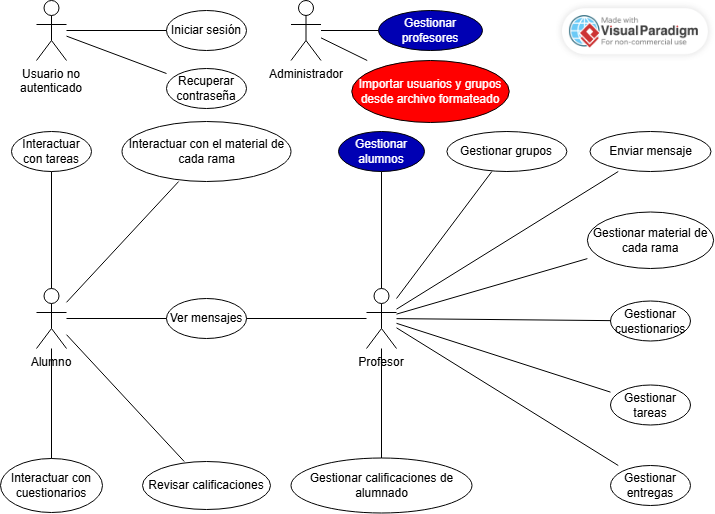
\includegraphics[width=1\linewidth]{Figuras/DCU_extendido.png}
     \caption{Diagrama UML de casos de uso del sistema extendido}
     \label{fig:dcu_extendido}
 \end{figure}

\section{Definición del diagrama de casos de uso}
\label{sec:def_dcu_ext}

Como se detalló en el trabajo previo, el diagrama ofrece una visión objetiva pero todavía abstracta del sistema. Para alcanzar un nivel operativo y verificable, se definen a continuación únicamente los casos de uso nuevos y aquellos existentes que se ven modificados por la incorporación de requisitos adicionales, manteniendo el resto de definiciones de la versión inicial sin cambios. Cabe destacar que se ha mantenido el mismo código de color para el nombre del caso de uso y se ha usado el color rojo en el resto de campos de los casos de uso que no son totalmente nuevos para indicar en qué cambian.

\subsection{Casos de uso nuevos o modificados}

\subsubsection{Caso de uso: Importar usuarios y grupos desde archivo formateado}
\begin{table}[H]
\centering
\begin{tabularx}{\textwidth}{
  |>{\centering\arraybackslash}l
  |>{\centering\arraybackslash}X|}
\hline
\textbf{Nombre} & {\textbf{\nuevo{Importar usuarios y grupos desde archivo formateado}}} \\ \hline
\textbf{Descripción} & Permitir al administrador crear usuarios y/o grupos mediante la carga de un fichero formateado, aplicando validaciones y creando relaciones de pertenencia según el contenido del archivo. \\ \hline
\textbf{Actor} & ACT-2 \\ \hline
\textbf{Requisitos funcionales} & RF-35 \\ \hline
\end{tabularx}
\caption{Caso de uso: Importar usuarios y grupos desde archivo formateado}
\end{table}

\subsubsection{Caso de uso que sustituye Crear profesor: Gestionar profesores}
\begin{table}[H]
\centering
\begin{tabularx}{\textwidth}{
  |>{\centering\arraybackslash}l
  |>{\centering\arraybackslash}X|}
\hline
\textbf{Nombre} & {\textbf{\cambiado{Gestionar profesores}}} \\ \hline
\textbf{Descripción} & Permitir al administrador crear\nuevo{, revisar y eliminar} usuarios con el rol de profesor en el sistema, proporcionando los datos necesarios y validando la información. \\ \hline
\textbf{Actor} & ACT-2 \\ \hline
\textbf{Requisitos funcionales} & RF-03 RF-04 \nuevo{RF-36} \nuevo{RF-37} \\ \hline
\end{tabularx}
\caption{Caso de uso: Gestionar profesores}
\end{table}

\subsubsection{Caso de uso que sustituye Crear alumno: Gestionar alumnos}
\begin{table}[H]
\centering
\begin{tabularx}{\textwidth}{
  |>{\centering\arraybackslash}l
  |>{\centering\arraybackslash}X|}
\hline
\textbf{Nombre} & {\textbf{\cambiado{Gestionar alumnos}}} \\ \hline
\textbf{Descripción} & Permitir al profesor crear\nuevo{, revisar y eliminar} usuarios con el rol de alumno en el sistema, proporcionando los datos necesarios y validando la información.\\ \hline
\textbf{Actor} & ACT-3 \\ \hline
\textbf{Requisitos funcionales} & RF-05 RF-04 \nuevo{RF-38} \nuevo{RF-39} \\ \hline
\end{tabularx}
\caption{Caso de uso: Gestionar alumnos}
\end{table}

\subsubsection{Caso de uso existente ampliado: Gestionar grupos}
\begin{table}[H]
\centering
\begin{tabularx}{\textwidth}{
  |>{\centering\arraybackslash}l
  |>{\centering\arraybackslash}X|}
\hline
\textbf{Nombre} & {\textbf{Gestionar grupos}} \\ \hline
\textbf{Descripción} & Permitir al profesor crear nuevos grupos, revisar los que ha creado y elegir un grupo para trabajar con él \nuevo{o eliminarlo}. \\ \hline
\textbf{Actor} & ACT-3 \\ \hline
\textbf{Requisitos funcionales} & RF-06 RF-07 RF-08 \nuevo{RF-40} \\ \hline
\end{tabularx}
\caption{Caso de uso: Gestionar grupos}
\end{table}
\subsubsection{Caso de uso existente ampliado: Interactuar con cuestionarios}
\begin{table}[H]
\centering
\begin{tabularx}{\textwidth}{
  |>{\centering\arraybackslash}l
  |>{\centering\arraybackslash}X|}
\hline
\textbf{Nombre} & {\textbf{Interactuar con cuestionarios}} \\ \hline
\textbf{Descripción} & Permitir al alumno interactuar con los cuestionarios. \\ \hline
\textbf{Actor} & ACT-4 \\ \hline
\textbf{Requisitos funcionales} & RF-18 RF-30 \nuevo{RF-41} \\ \hline
\end{tabularx}
\caption{Caso de uso: Interactuar con cuestionarios}
\end{table}

\subsection{Requisitos funcionales nuevos}
\label{sec:rf_extensiones}

En coherencia con el documento original, los identificadores continúan a partir del último requisito definido. A continuación se describen únicamente los nuevos requisitos y las ampliaciones necesarias de los casos de uso afectados.

\begin{table}[H]
\centering
\begin{tabularx}{\textwidth}{
  |>{\centering\arraybackslash}l
  |>{\centering\arraybackslash}X|}
\hline
\textbf{RF-35} & \textbf{Importar usuarios y grupos desde archivo formateado} \\ \hline
\textbf{Descripción} & Permitir al administrador crear usuarios y/o grupos mediante la carga de un fichero formateado, aplicando validaciones y creando relaciones de pertenencia según el contenido del archivo. \\ \hline
\textbf{Precondición} & El administrador debe estar autenticado y disponer de un fichero válido según el formato establecido. \\ \hline
\textbf{Secuencia de pasos} &
\begin{enumerate}
  \item El administrador accede a la opción de importación dentro del área de administración.
  \item El administrador selecciona un fichero local para cargar.
  \item El sistema valida el formato general del fichero (estructura, campos obligatorios y consistencia).
  \item El sistema recorre los registros y valida datos (equivalente a RF-04 cuando aplique), incluyendo unicidad de correos y reglas de generación de credenciales.
  \item El sistema crea los usuarios y grupos indicados si todos han sido validados.
  \item El sistema informa del éxito.
\end{enumerate} \\ \hline
\textbf{Postcondición} & Los usuarios y grupos quedan registrados y listos para su uso. \\ \hline
\textbf{Excepciones} &
\begin{itemize}
  \item El fichero no cumple el formato establecido o falta información obligatoria.
  \item Existen registros con correos duplicados o datos inválidos.
  \item Problemas de conexión con la base de datos.
\end{itemize} \\ \hline
\end{tabularx}
\caption{{Requisito funcional: RF-35 Importar usuarios y grupos desde archivo formateado}}
\end{table}

\begin{table}[H]
\centering
\begin{tabularx}{\textwidth}{
  |>{\centering\arraybackslash}l
  |>{\centering\arraybackslash}X|}
\hline
\textbf{RF-36} & \textbf{Revisar profesores} \\ \hline
\textbf{Descripción} & Permitir al administrador visualizar la lista de profesores registrados en el sistema y acceder a su información básica para su gestión. \\ \hline
\textbf{Precondición} & El administrador debe estar autenticado y tener profesores creados. \\ \hline
\textbf{Secuencia de pasos} &
\begin{enumerate}
  \item El administrador entra en la sección de profesores.
  \item El sistema recupera y muestra el listado de profesores registrados.
\end{enumerate} \\ \hline
\textbf{Postcondición} & El administrador puede identificar profesores gestionables y realizar acciones de creación o eliminación desde el mismo contexto. \\ \hline
\textbf{Excepciones} &
\begin{itemize}
  \item No existen profesores registrados.
  \item Problemas de conexión a la base de datos.
\end{itemize} \\ \hline
\end{tabularx}
\caption{Requisito funcional: RF-36 Revisar profesores}
\end{table}

\begin{table}[H]
\centering
\begin{tabularx}{\textwidth}{
  |>{\centering\arraybackslash}l
  |>{\centering\arraybackslash}X|}
\hline
\textbf{RF-37} & \textbf{Eliminar profesor} \\ \hline
\textbf{Descripción} & Permitir al administrador eliminar un profesor del sistema, eliminando todo su material asociado (tareas, cuestionarios, ramas, entregas y
calificaciones), sus grupos y los alumnos creados bajo su responsabilidad, evitando referencias huérfanas o inconsistencias. \\ \hline
\textbf{Precondición} & El administrador debe estar autenticado y el profesor a eliminar debe existir. \\ \hline
\textbf{Secuencia de pasos} &
\begin{enumerate}
  \item El administrador accede a la administración de profesores y visualiza el listado.
  \item El administrador selecciona un profesor y solicita su eliminación.
  \item El sistema muestra confirmación.
  \item El administrador confirma.
  \item El sistema elimina al profesor y todos los datos relacionados con él.
  \item El sistema informa del éxito.
\end{enumerate} \\ \hline
\textbf{Postcondición} & El profesor deja de existir en el sistema y sus recursos asociados quedan gestionados de forma consistente. \\ \hline
\textbf{Excepciones} &
\begin{itemize}
  \item El profesor no existe.
  \item Problemas de conexión a la base de datos.
\end{itemize} \\ \hline
\end{tabularx}
\caption{Requisito funcional: RF-37 Eliminar profesor}
\end{table}

\begin{table}[H]
\centering
\begin{tabularx}{\textwidth}{
  |>{\centering\arraybackslash}l
  |>{\centering\arraybackslash}X|}
\hline
\textbf{RF-38} & \textbf{Revisar alumnos} \\ \hline
\textbf{Descripción} & Permitir al profesor visualizar la lista de alumnos creados por él y acceder a su información básica para su gestión. \\ \hline
\textbf{Precondición} & El profesor debe estar autenticado y tener alumnos creados. \\ \hline
\textbf{Secuencia de pasos} &
\begin{enumerate}
  \item El profesor accede al área de administración y entra en la sección de alumnos.
  \item El sistema recupera y muestra el listado de alumnos del profesor.
\end{enumerate} \\ \hline
\textbf{Postcondición} & El profesor puede identificar a los alumnos gestionables y realizar acciones de creación o eliminación desde el mismo contexto. \\ \hline
\textbf{Excepciones} &
\begin{itemize}
  \item No existen alumnos creados por el profesor.
  \item Problemas de conexión a la base de datos.
\end{itemize} \\ \hline
\end{tabularx}
\caption{Requisito funcional: RF-38 Revisar alumnos}
\end{table}

\begin{table}[H]
\centering
\begin{tabularx}{\textwidth}{
  |>{\centering\arraybackslash}l
  |>{\centering\arraybackslash}X|}
\hline
\textbf{RF-39} & \textbf{Eliminar alumno} \\ \hline
\textbf{Descripción} & Permitir al profesor eliminar un alumno creado por él, garantizando que el sistema gestiona de forma consistente la información asociada exclusivamente al alumno (calificaciones y entregas). \\ \hline
\textbf{Precondición} & El profesor debe estar autenticado y el alumno a eliminar debe haber sido creado previamente por el profesor. \\ \hline
\textbf{Secuencia de pasos} &
\begin{enumerate}
  \item El profesor accede al área de administración y visualiza el listado de alumnos gestionables.
  \item El profesor selecciona un alumno y solicita su eliminación.
  \item El sistema muestra un aviso de confirmación describiendo el alcance de la operación.
  \item El profesor confirma la eliminación.
  \item El sistema elimina el alumno, los datos exclusivos del alumno y las relaciones del alumno en el resto de registros que figure para mantener la consistencia.
  \item El sistema informa del éxito.
\end{enumerate} \\ \hline
\textbf{Postcondición} & El alumno deja de existir en el sistema y no es accesible desde la interfaz, por lo tanto, los datos asociados quedan en un estado consistente. \\ \hline
\textbf{Excepciones} &
\begin{itemize}
  \item {El alumno no existe o no ha sido creado por el profesor autenticado.}
  \item {Problemas de conexión a la base de datos.}
\end{itemize} \\ \hline
\end{tabularx}
\caption{Requisito funcional: RF-39 Eliminar alumno}
\end{table}

\begin{table}[H]
\centering
\begin{tabularx}{\textwidth}{
  |>{\centering\arraybackslash}l
  |>{\centering\arraybackslash}X|}
\hline
\textbf{RF-40} & \textbf{Eliminar grupo} \\ \hline
\textbf{Descripción} & Permitir al profesor eliminar un grupo creado por él, gestionando de forma consistente todo el material asociado (tareas, cuestionarios, ramas, entregas y calificaciones). \\ \hline
\textbf{Precondición} & El profesor debe estar autenticado y el grupo a eliminar debe haber sido creado previamente por el profesor. \\ \hline
\textbf{Secuencia de pasos} &
\begin{enumerate}
  \item El profesor visualiza su listado de grupos y selecciona el grupo a eliminar.
  \item El profesor solicita la eliminación del grupo.
  \item El sistema solicita confirmación, indicando que se trata de una eliminación irreversible.
  \item El profesor confirma.
  \item El sistema elimina el grupo y todos los datos relacionados con el grupo menos los usuarios.
  \item El sistema informa del éxito.
\end{enumerate} \\ \hline
\textbf{Postcondición} & El grupo deja de existir en el sistema y no puede seleccionarse, además, no quedan recursos asociados accesibles de forma inconsistente. \\ \hline
\textbf{Excepciones} &
\begin{itemize}
  \item El grupo no existe o no ha sido creado por el profesor autenticado.
  \item Problemas de conexión a la base de datos.
\end{itemize} \\ \hline
\end{tabularx}
\caption{Requisito funcional: RF-40 Eliminar grupo}
\end{table}

\begin{table}[H]
\centering
\begin{tabularx}{\textwidth}{
  |>{\centering\arraybackslash}l
  |>{\centering\arraybackslash}X|}
\hline
\textbf{RF-41} & \textbf{Solicitar pista durante un cuestionario} \\ \hline
\textbf{Descripción} & Permitir al alumno solicitar solo una pista asociada a una pregunta concreta durante la realización de un cuestionario, recibiendo una orientación limitada que facilite el razonamiento sin revelar la respuesta. \\ \hline
\textbf{Precondición} & El alumno debe estar autenticado, haber accedido a un cuestionario activo y encontrarse en el proceso de respuesta. \\ \hline
\textbf{Secuencia de pasos} &
\begin{enumerate}
  \item El sistema muestra las preguntas del cuestionario.
  \item El alumno solicita una pista para la pregunta que tenga dudas.
  \item El sistema presenta una pista contextual (orientación), sin mostrar directamente la opción correcta.
  \item El alumno continúa respondiendo a la pregunta.
  \item El sistema permite finalizar y entregar el cuestionario como en RF-30.
\end{enumerate} \\ \hline
\textbf{Postcondición} & El alumno recibe una pista y puede continuar la realización de la entrega bajo las reglas de RF-30. \\ \hline
\textbf{Excepciones} &
\begin{itemize}
  \item El cuestionario no está activo o el alumno no tiene acceso al mismo.
  \item El servicio de generación de pista no está disponible.
  \item Problemas de conexión a la base de datos.
\end{itemize} \\ \hline
\end{tabularx}
\caption{Requisito funcional: RF-41 Solicitar pista durante un cuestionario}
\end{table}

\section{Requisitos no funcionales nuevos}
\label{sec:rnf_ext}

El proyecto original definía un requisito de portabilidad (RNF-04) orientado a asegurar que la aplicación pudiera utilizarse en distintos dispositivos y entornos. En este complemento, esa portabilidad se concreta en un objetivo más exigente y verificable: la exportación efectiva a un entorno móvil Android, aprovechando el diseño híbrido y responsive \cite{UNIRResponsive} ya adoptado.

\begin{table}[H]
\centering
\begin{tabularx}{\textwidth}{
  |>{\centering\arraybackslash}l
  |>{\centering\arraybackslash}X|}
\hline
\textbf{RNF-08} & \textbf{Portabilidad a Android} \\ \hline
\textbf{Descripción} & El sistema deberá poder ejecutarse como aplicación instalada en dispositivos Android, manteniendo las funcionalidades esenciales y una experiencia de usuario consistente. \\ \hline
\textbf{Justificación} & Se da continuidad a RNF-04 (Portabilidad) del proyecto base, materializando la ejecución en un entorno móvil real para reforzar accesibilidad y facilitar su implantación en contextos educativos. \\ \hline
\textbf{Criterio de cumplimiento} & La aplicación se exporta y ejecuta en Android mediante herramientas de construcción móvil, pudiendo autenticarse, navegar por ramas, consultar materiales y realizar acciones principales sin degradación funcional. \\ \hline
\end{tabularx}
\caption{Requisito no funcional: RNF-08 Portabilidad a Android}
\end{table}

\section{Arquitectura e implementación de la solución}
\label{sec:arquitectura_implementacion}

Una vez definida la solución extendida desde el punto de vista funcional, resulta necesario describir cómo se han materializado técnicamente las nuevas capacidades incorporadas durante este complemento. Para ello, se mantiene como punto de partida la arquitectura desarrollada en el Trabajo Fin de Grado, evitando replantear una solución que ya había sido validada y centrando el esfuerzo en su evolución controlada.

La aplicación conserva una arquitectura cliente-servidor basada en una \textbf{API REST}, con un backend desarrollado mediante \textbf{Node.js} y \textbf{Express}, un frontend híbrido construido con \textbf{Ionic} y \textbf{Angular}, y una base de datos documental \textbf{MongoDB}. Esta continuidad tecnológica permite integrar las nuevas funcionalidades sin alterar la estructura general del sistema, manteniendo los principios de modularidad, separación de responsabilidades y escalabilidad definidos en la versión base.

Dentro de esta evolución técnica se distinguen tres ámbitos principales. En primer lugar, el backend se amplía para soportar nuevas operaciones de gestión, importación masiva de datos, eliminaciones consistentes e integración con servicios externos. En segundo lugar, el frontend se adapta para incorporar las nuevas funcionalidades y mejorar su comportamiento en dispositivos móviles. Finalmente, el despliegue se extiende para contemplar no solo la versión web, sino también la generación de una aplicación instalable en Android.

\subsection{Implementación del backend}
\label{sec:backend_impl}

El backend de la solución extendida se apoya directamente en la base implementada en la versión inicial, manteniendo la misma pila tecnológica: \textbf{Node.js} como entorno de ejecución y \textbf{Express} como framework para exponer una \textbf{API REST}. A nivel de organización interna, se conserva la separación de responsabilidades típica de la versión anterior, con una estructura inspirada en \textbf{MVC adaptado a backend} sin capa de interfaz: \textbf{modelos} para la persistencia y el esquema de datos, \textbf{controladores} para la lógica de operaciones y \textbf{rutas} como capa de entrada a los endpoints.

En esta fase del complemento, la evolución del backend no se centra únicamente en añadir operaciones CRUD aisladas, sino en reforzar funcionalidades necesarias en un uso real de la aplicación. Las nuevas capacidades requieren mayor validación, limpieza de relaciones, control de errores y coherencia en operaciones que afectan a varias entidades del sistema.

Además, se incorpora una pieza nueva dentro de la organización del backend: la capa de \textbf{servicios}. Esta capa se utiliza para encapsular integraciones externas, como la comunicación con la \textbf{API de Groq}, evitando mezclar la lógica de negocio propia de la aplicación con dependencias externas y facilitando así el mantenimiento futuro.

\subsubsection{Modelado de datos}

Con el objetivo de proporcionar una visión global de la estructura de la información manejada por el sistema, se elaboró en el sistema base un modelo conceptual de datos que identifica las principales entidades del dominio y las relaciones existentes entre ellas. Este modelo permite comprender de forma clara cómo se organiza la información dentro de la aplicación y sirve como referencia para la posterior implementación de la persistencia de datos en el backend.

Es importante recordar que el diagrama presentado no corresponde a un diagrama Entidad-Relación en sentido estricto. En su lugar, se adopta un enfoque conceptual que refleja la estructura lógica de los datos y sus relaciones semánticas, independientemente de su implementación física.

La Figura~\ref{fig:modelo_conceptual} muestra el modelo conceptual de datos del sistema, proporcionando una visión estructural que complementa la definición funcional y arquitectónica presentada en los apartados anteriores.

\begin{figure}[H]
    \centering
    
\includegraphics[width=\textwidth]{Figuras/modelo_Conceptual.png}
    \caption{Modelo conceptual de datos del sistema}
    \label{fig:modelo_conceptual}
\end{figure}

\newpage

\subsubsection{Implementación}

La implementación del backend se centra en materializar las nuevas funcionalidades definidas previamente, manteniendo la arquitectura ya existente y ampliando únicamente aquellos elementos necesarios para dar soporte a los nuevos requisitos. En concreto, las principales actuaciones realizadas se agrupan en tres bloques: operaciones lógicas de revisión y eliminación, importación masiva desde CSV e integración con servicios externos de inteligencia artificial.

\paragraph{Operaciones lógicas de revisión y eliminación}

Las operaciones de revisión, como listados y consultas, reutilizan el mismo patrón del trabajo previo: filtrado por rol, respuesta en formato JSON \cite{RFC8259} y acceso a través de controladores. En cambio, las eliminaciones se han ampliado para contemplar el efecto real que estas operaciones tienen sobre otras colecciones relacionadas.

Por ejemplo, al eliminar un grupo no basta con borrar el documento principal correspondiente, ya que dicho grupo puede tener asociadas tareas, cuestionarios, entregas y calificaciones. Por tanto, la operación debe garantizar que el sistema no conserva referencias huérfanas ni información inconsistente.

Se incluye a continuación un ejemplo representativo. El resto de eliminaciones sigue una estructura muy similar, adaptando la limpieza de relaciones a cada entidad concreta.

\begin{Verbatim}[frame=single, fontsize=\small, xleftmargin=10pt, xrightmargin=10pt]
// Ejemplo representativo: eliminar un grupo y limpiar datos asociados
async function eliminarGrupo(groupId, profesorId) {
  //1) Verificar que el grupo existe y pertenece al profesor autenticado
  const grupo = await Grupo.findOne({
    _id: groupId,
    profesor: profesorId
  });

  if (!grupo) {
    throw new Error('Grupo no encontrado o sin permisos');
  }
  //2) Eliminar contenido asociado al grupo
  await Tarea.deleteMany({ grupo: groupId });
  await Cuestionario.deleteMany({ grupo: groupId });

  //3) Eliminar entregas y calificaciones asociadas
  await Entrega.deleteMany({ grupo: groupId });
  await Calificacion.deleteMany({ grupo: groupId });

  //4) Eliminar el documento principal
  await Grupo.deleteOne({ _id: groupId });
  // Las relaciones también quedan eliminadas
  return { ok: true };
}
\end{Verbatim}

Este planteamiento permite que las operaciones destructivas se ejecuten de manera controlada, respetando los permisos del usuario autenticado y garantizando la coherencia de los datos almacenados.

\paragraph{Importación masiva desde CSV: normalización, validación y creación}

La importación masiva desde CSV \cite{RFC4180CSVValidation} introduce un flujo distinto al alta individual, ya que los datos provienen de una fuente externa y pueden contener errores, duplicados o referencias inconsistentes. Por este motivo, el proceso se ha diseñado siguiendo un enfoque estrictamente controlado, dividido en dos fases claramente diferenciadas.

\begin{itemize}
  \item \textbf{Validación completa previa}: el archivo CSV se parsea y se recorren todas las filas sin crear ningún elemento en la base de datos. Durante esta fase se validan campos obligatorios, duplicados internos, referencias cruzadas entre usuarios y grupos, y se comprueba la coherencia con las reglas de negocio del sistema.
  \item \textbf{Creación atómica}: únicamente si la validación finaliza sin errores, se procede a la creación de usuarios y grupos dentro de una transacción de Mongoose, garantizando que el proceso se complete íntegramente o se revierta completamente en caso de fallo \cite{MongooseTransactions}.
\end{itemize}

Además, se aplica una regla del sistema clave en este complemento: \textbf{un alumno pertenece a un único profesor}. Esto se comprueba antes de crear los grupos; si un grupo de un profesor intenta incluir un alumno asignado a otro profesor, se detiene la importación.

Este enfoque permite detectar todos los errores del CSV de forma anticipada y evita la creación parcial de datos, asegurando la consistencia del sistema incluso ante archivos mal formateados o incompletos. Dado que la implementación completa de este proceso resulta extensa y muy dependiente de detalles técnicos, se ha optado por presentar un código conceptual que resume el flujo principal, facilitando su comprensión sin perder el significado funcional.

\begin{Verbatim}[frame=single, fontsize=\small, xleftmargin=10pt, xrightmargin=10pt]

func importarDesdeCSV(archivoCSV):

  filas <- parsearCSV(archivoCSV)
  errores <- []

  // Fase 1: validación completa
  para cada fila en filas:
    validarCamposObligatorios(fila)
    validarDuplicadosInternos(fila)
    validarReferencias(fila)
    aplicarReglasDeNegocio(fila)
    acumularErrores(errores)

  si errores no está vacío:
    devolver errores y cancelar proceso

  // Fase 2: creación atómica
  iniciarTransacción()

  crearProfesores()
  crearAlumnos(asignados a su profesor)
  crearGrupos(verificando coherencia)

  confirmarTransacción()

  enviarCorreosConCredenciales()
  devolver resultado de éxito
\end{Verbatim}

La división del proceso en una fase de validación y otra de creación permite que la importación funcione como una operación segura y predecible. De esta forma, se reduce la carga administrativa asociada al alta manual de usuarios y grupos, pero sin comprometer la integridad de la información almacenada en la base de datos.

\paragraph{Integración del servicio de inteligencia artificial mediante Groq}

Una de las principales novedades incorporadas en este complemento es la integración de un servicio externo de inteligencia artificial capaz de generar pistas para las preguntas de los cuestionarios. Esta funcionalidad responde al objetivo de ofrecer al alumnado un mecanismo de ayuda durante la realización de actividades evaluables sin comprometer el carácter formativo de las mismas.

Desde el punto de vista arquitectónico, esta integración no se incorpora directamente en los controladores, sino que se implementa mediante una capa específica de \textbf{servicios}. Esta decisión permite desacoplar completamente la lógica de negocio propia de la aplicación de la comunicación con proveedores externos, facilitando el mantenimiento del sistema y permitiendo sustituir el servicio utilizado en el futuro sin afectar al resto de la arquitectura.

La comunicación con Groq se realiza mediante su API pública. El backend construye dinámicamente un \textit{prompt} \cite{PromptEngineeringGuide} que incluye la pregunta, las posibles respuestas y una serie de restricciones destinadas a evitar que el modelo revele directamente la solución. Una vez recibida la respuesta, esta es validada, procesada y enviada al frontend como una pista contextual para el alumno.

A continuación se muestra el fragmento principal encargado de generar dichas pistas.

\begin{Verbatim}[frame=single, fontsize=\small, xleftmargin=10pt, xrightmargin=10pt]
// Importación del SDK oficial de Groq para realizar peticiones
// al servicio de inferencia mediante su API
const Groq = require('groq-sdk');

// Inicialización del cliente de Groq utilizando la clave
// de API definida en las variables de entorno
const groq = new Groq({ apiKey: process.env.GROQ_API_KEY });

// Función asíncrona encargada de generar una pista teórica
// breve para una pregunta tipo test
async function generarPistaTeoria({
  preguntaTexto,
  posiblesRespuestas,
  recursoAudicion
}) {

// Comprobación previa de la existencia de la clave de API.
// Si no está configurada, se interrumpe la ejecución
  if (!process.env.GROQ_API_KEY) {
    throw new Error('GROQ_API_KEY no está configurada');
  }

// Construcción del bloque de opciones en formato texto.
// Se numeran las respuestas y se evita provocar errores
// en caso de que algún elemento no tenga texto definido
  const opciones = Array.isArray(posiblesRespuestas)
    ? posiblesRespuestas
        .map((r, i) => `${i + 1}) ${r?.texto ?? ''}`)
        .join('\n')
    : '';

  const userContent =
`Genera UNA pista breve para ayudar a responder esta pregunta tipo test
sin revelar la respuesta.

Pregunta:
${preguntaTexto}

Opciones:
${opciones}

${recursoAudicion ? 'Hay un recurso de audición asociado.' : ''}

Requisitos:
- 1 o 2 frases máximo
- No digas cuál es la opción correcta
- No des la solución ni pasos completos
- No menciones "IA" ni "modelo"`;

  const completion = await groq.chat.completions.create({
    model: 'llama-3.3-70b-versatile',
    messages: [
      { role: 'system',
        content: 'Eres un tutor de música. Das pistas breves y seguras.' },
      { role: 'user',
        content: userContent }
    ],
    temperature: 0.2,
    max_tokens: 90
  });

  const hint =
    completion?.choices?.[0]?.message?.content?.trim();

  if (!hint) throw new Error('No se pudo generar pista');

  return hint
    .replace(/^["'\s]+|["'\s]+$/g, '')
    .trim();
}

module.exports = { generarPistaTeoria };
\end{Verbatim}

La utilización de una capa de servicios permite encapsular toda la comunicación con el modelo de inteligencia artificial en un único punto del sistema. De esta forma, el resto de componentes del backend únicamente solicitan una pista cuando la necesitan, permaneciendo completamente independientes de la tecnología utilizada para generarla.

\subsubsection{Testing}

El backend mantiene el enfoque de pruebas definido en el proyecto base, utilizando \textbf{Jest} como framework de testing unitario y \textbf{Supertest} para la validación de los distintos endpoints de la API REST. Esta combinación permite comprobar tanto la correcta implementación de la lógica de negocio como el comportamiento observable desde el punto de vista del cliente.

Sobre esta base consolidada, la solución extendida incorpora nuevos escenarios de prueba derivados de las funcionalidades añadidas durante este complemento. En particular, se presta especial atención a aquellos procesos que presentan una mayor complejidad lógica o que afectan directamente a la consistencia de la información almacenada.

Las pruebas desarrolladas verifican, entre otros aspectos:

\begin{itemize}
    \item El correcto funcionamiento del proceso de importación masiva desde archivos CSV, validando tanto los casos de éxito como los distintos escenarios de error derivados de datos inconsistentes o referencias inválidas.
    \item La correcta ejecución de las operaciones de eliminación, garantizando que los datos relacionados sean eliminados de forma coherente y no permanezcan referencias huérfanas en el sistema.
    \item La integración con el servicio de inteligencia artificial encargado de generar pistas para los cuestionarios, comprobando tanto el funcionamiento normal como las situaciones de indisponibilidad del servicio externo.
\end{itemize}

Para ello, se mantiene la estrategia de aislamiento empleada en la versión inicial mediante el uso de \textit{mocks} y \textit{spies}, permitiendo simular de forma controlada tanto el acceso a la base de datos como el comportamiento de servicios externos. Asimismo, Supertest facilita la ejecución de peticiones HTTP reales contra la aplicación, verificando los códigos de estado y el contenido de las respuestas devueltas.

Como ejemplo representativo se presenta el conjunto de pruebas desarrollado para el endpoint encargado de obtener una pista asociada a una pregunta concreta, accesible mediante la ruta 

\texttt{GET /cuestionarios/:id/preguntas/:index/pista}. 

Este endpoint resulta especialmente interesante debido a que combina la lógica propia del backend con la interacción con un servicio externo de inteligencia artificial.

\begin{Verbatim}[frame=single, fontsize=\small, xleftmargin=10pt, xrightmargin=10pt]
// Bloque de pruebas para el endpoint encargado de
// devolver una pista asociada a una pregunta concreta
describe('GET /cuestionarios/:id/preguntas/:index/pista', () => {

  it('200 - devuelve pista', async () => {

    jest.spyOn(cuestionarioController, 'getPistaPregunta')
      .mockResolvedValue({
        status: 200,
        body: { pista: 'PISTA', cached: true }
      });

    const res = await request(app)
      .get('/cuestionarios/c1/preguntas/0/pista');

    expect(res.status).toBe(200);
    expect(res.body.pista).toBe('PISTA');
  });

  it('400 - preguntaIndex inválido', async () => {

    const res = await request(app)
      .get('/cuestionarios/c1/preguntas/abc/pista');

    expect(res.status).toBe(400);
  });

  it('503 - mantenimiento', async () => {

    jest.spyOn(cuestionarioController, 'getPistaPregunta')
      .mockResolvedValue({
        status: 503,
        body: { error: 'Pistas en mantenimiento.' }
      });

    const res = await request(app)
      .get('/cuestionarios/c1/preguntas/0/pista');

    expect(res.status).toBe(503);
  });
});

\end{Verbatim}

Este conjunto de pruebas permite comprobar de forma sistemática el comportamiento del nuevo servicio de generación de pistas tanto en condiciones normales como ante situaciones de error. Con ello se garantiza que la incorporación de esta nueva funcionalidad no compromete la estabilidad del backend y mantiene el mismo nivel de calidad y fiabilidad alcanzado en la versión inicial del proyecto.

\subsection{Implementación del frontend}
\label{sec:frontend_impl}

La implementación del frontend mantiene la pila tecnológica definida en el proyecto original, basada en \textbf{Angular} e \textbf{Ionic}. Angular continúa proporcionando una arquitectura modular organizada mediante componentes, servicios y módulos, mientras que Ionic aporta una biblioteca de componentes orientada al desarrollo de interfaces adaptables tanto a navegadores como a dispositivos móviles.

Desde el punto de vista arquitectónico, se conserva el esquema empleado en la versión inicial, en el que los componentes son responsables de la gestión del estado y la interacción con el usuario, los servicios encapsulan la comunicación con la API REST y la lógica reutilizable, y las interfaces representan las estructuras de datos intercambiadas entre el frontend y el backend.

Las nuevas funcionalidades incorporadas durante este complemento se integran sobre esta arquitectura sin introducir cambios estructurales. La principal evolución del frontend se centra en dos aspectos: la incorporación de las nuevas funcionalidades definidas en la solución extendida y la adaptación de la aplicación para su ejecución como aplicación instalada en dispositivos Android.

\subsubsection{Exportación a Android mediante Capacitor}

La principal ampliación realizada sobre el frontend consiste en la incorporación de \textbf{Capacitor} como puente entre la aplicación web y el sistema operativo móvil. Gracias a esta herramienta, la aplicación desarrollada con Ionic y Angular puede ejecutarse como una aplicación instalada, reutilizando completamente el código existente y evitando desarrollar una aplicación nativa independiente.

Desde el punto de vista práctico, Capacitor permite:

\begin{itemize}
    \item Generar un contenedor Android para ejecutar la aplicación como software instalado.
    \item Acceder a funcionalidades propias del dispositivo mediante plugins nativos.
    \item Adaptar determinados comportamientos de la interfaz que difieren respecto a la ejecución en un navegador web.
\end{itemize}

Esta aproximación mantiene una única base de código para ambas plataformas, reduciendo el esfuerzo de mantenimiento y garantizando una experiencia homogénea para todos los usuarios.

\paragraph{Adaptación a los elementos propios del sistema operativo}

Uno de los primeros ajustes realizados consiste en adaptar correctamente la interfaz a los elementos propios del sistema operativo móvil, como la barra superior de estado o la barra de navegación inferior.

Para ello se utilizan los plugins proporcionados por Capacitor, permitiendo controlar el comportamiento de la barra de estado y evitando que ésta se superponga sobre la interfaz desarrollada con Ionic.

\begin{Verbatim}[frame=single, fontsize=\small, xleftmargin=10pt, xrightmargin=10pt]
if (this.platform.is('capacitor')) {

  await StatusBar.setOverlaysWebView({ overlay: false });

  await StatusBar.setStyle({ style: Style.Default });
}
\end{Verbatim}

Como complemento, también se emplean las denominadas \textit{safe areas} proporcionadas por el propio sistema operativo. Estas variables permiten adaptar automáticamente los márgenes interiores de la aplicación en función del dispositivo utilizado, evitando solapes independientemente del tamaño de pantalla o de la presencia de menús propios del sistema.

\begin{Verbatim}[frame=single, fontsize=\small, xleftmargin=10pt, xrightmargin=10pt]
body {
  padding-top: env(safe-area-inset-top);
  padding-bottom: env(safe-area-inset-bottom);
  padding-left: env(safe-area-inset-left);
  padding-right: env(safe-area-inset-right);
}
\end{Verbatim}

\paragraph{Gestión de documentos PDF}

Otra de las adaptaciones necesarias afecta a la visualización de documentos PDF.

Mientras que en un navegador web resulta habitual utilizar un elemento \texttt{iframe} para visualizar directamente el documento, este comportamiento no siempre está disponible cuando la aplicación se ejecuta dentro del WebView de Android.

La solución adoptada consiste en almacenar temporalmente el documento mediante el plugin \texttt{Filesystem} y abrirlo posteriormente utilizando el visor PDF instalado en el propio dispositivo mediante el plugin \texttt{FileOpener}. De esta forma, el usuario obtiene una experiencia equivalente a la de cualquier otra aplicación móvil.

El siguiente fragmento muestra el funcionamiento implementado para el libro del curso de cada rama.

\begin{Verbatim}[frame=single, fontsize=\small, xleftmargin=10pt, xrightmargin=10pt]
//Se comprueba al inicio si es pantalla reducida
@HostListener('window:resize')
onResize() {
  this.checkIsMobile();
}

private checkIsMobile(): void {
  this.isMobile = window.matchMedia('(max-width: 1368px)').matches;
}

async openPdf(): Promise<void> {

  try {

    if (!this.libroBlob) {
      await this.presentToast(
      'No hay PDF disponible para abrir.', 'danger');
      return;
    }

    const base64 = await this.blobToBase64(this.libroBlob);

    const fileName =
    `libro-apoyo-${this.ramaConfig?._id || 'rama'}.pdf`;

    const result = await Filesystem.writeFile({
      path: fileName,
      data: base64,
      directory: Directory.Cache,
      recursive: true,
    });

    await FileOpener.open({
      filePath: result.uri,
      contentType: 'application/pdf',
      openWithDefault: true,
    });

  } catch (e) {

    console.error(e);

    await this.presentToast(
    'No se pudo abrir el PDF en este dispositivo.',
    'danger');

  }
}
\end{Verbatim}

La utilización de estos plugins permite aprovechar las capacidades nativas del dispositivo manteniendo la lógica de negocio completamente compartida entre la versión web y la versión Android.

\paragraph{Adaptación de la interfaz a pantallas reducidas}

La exportación a dispositivos móviles también ha requerido pequeños ajustes en determinados componentes visuales cuya disposición original estaba pensada para pantallas de mayor tamaño.

Uno de los casos más representativos corresponde al conjunto de acciones disponibles para el profesorado en la gestión de tareas. En la versión web estos controles se muestran simultáneamente mediante varios botones, mientras que en dispositivos móviles pasan a agruparse en un único botón desplegable para preservar el espacio disponible.

Esta adaptación se realiza mediante reglas CSS apoyadas en consultas \texttt{@media}, permitiendo que el propio navegador seleccione automáticamente la distribución adecuada.

\begin{Verbatim}[frame=single, fontsize=\small, xleftmargin=10pt, xrightmargin=10pt]
@media (max-width: 767px) {

  .desktop-only {
    display: none;
  }

  .mobile-only {
    display: flex;
  }

}

.desktop-only {
  display: flex;
}

.mobile-only {
  display: none;
}
\end{Verbatim}

Este tipo de modificaciones resulta reducido gracias a la utilización conjunta de Ionic y Capacitor, ya que la mayor parte de los componentes proporcionan un comportamiento adaptativo de forma automática.

\paragraph{Configuración final mediante Android Studio}

Una vez generado el proyecto Android mediante Capacitor, Android Studio se emplea para realizar los ajustes finales específicos de la plataforma.

Entre ellos destacan la configuración del icono de la aplicación, la personalización de la pantalla de carga, la definición de permisos y la edición de los archivos XML utilizados por Android para describir la aplicación instalada.

Estos ajustes permiten que la aplicación presente un comportamiento y una apariencia completamente integrados con el sistema operativo, reforzando la percepción de producto final y mejorando la experiencia de usuario.

\subsubsection{Diseño y experiencia de usuario (UX/UI)}
\label{sec:frontend_diseno_ext}

La evolución del frontend no implica un rediseño completo de la interfaz desarrollada en el proyecto original. La identidad visual, la organización de la navegación y los principales patrones de interacción se mantienen, ya que fueron definidos específicamente para adaptarse al proceso de enseñanza del lenguaje musical y demostraron un comportamiento satisfactorio durante el desarrollo de la versión inicial.

En este complemento, el trabajo realizado desde el punto de vista de la experiencia de usuario se centra en adaptar la interfaz al nuevo entorno de ejecución móvil y en garantizar que las nuevas funcionalidades incorporadas mantengan la misma coherencia visual que el resto del sistema.

\paragraph{Continuidad visual entre plataformas}

Uno de los principales objetivos perseguidos durante esta evolución ha sido preservar una experiencia homogénea independientemente del dispositivo utilizado. Gracias a la utilización conjunta de Angular, Ionic y Capacitor, la estructura general de navegación permanece inalterada tanto en la versión web como en la aplicación Android.

En consecuencia:

\begin{itemize}
    \item Se mantiene la organización funcional de la aplicación, diferenciando claramente las zonas de navegación académica y las tareas administrativas.
    \item Se conservan los patrones de interacción empleados en la versión inicial, utilizando listas dinámicas, formularios, ventanas modales y notificaciones emergentes de manera consistente.
    \item La identidad gráfica permanece unificada entre plataformas, reforzando la percepción de una única aplicación independientemente del entorno desde el que se utilice.
\end{itemize}

La Figura~\ref{fig:menus} muestra la organización general de los menús de navegación utilizada en la aplicación.

\begin{figure}[H]
  \centering
  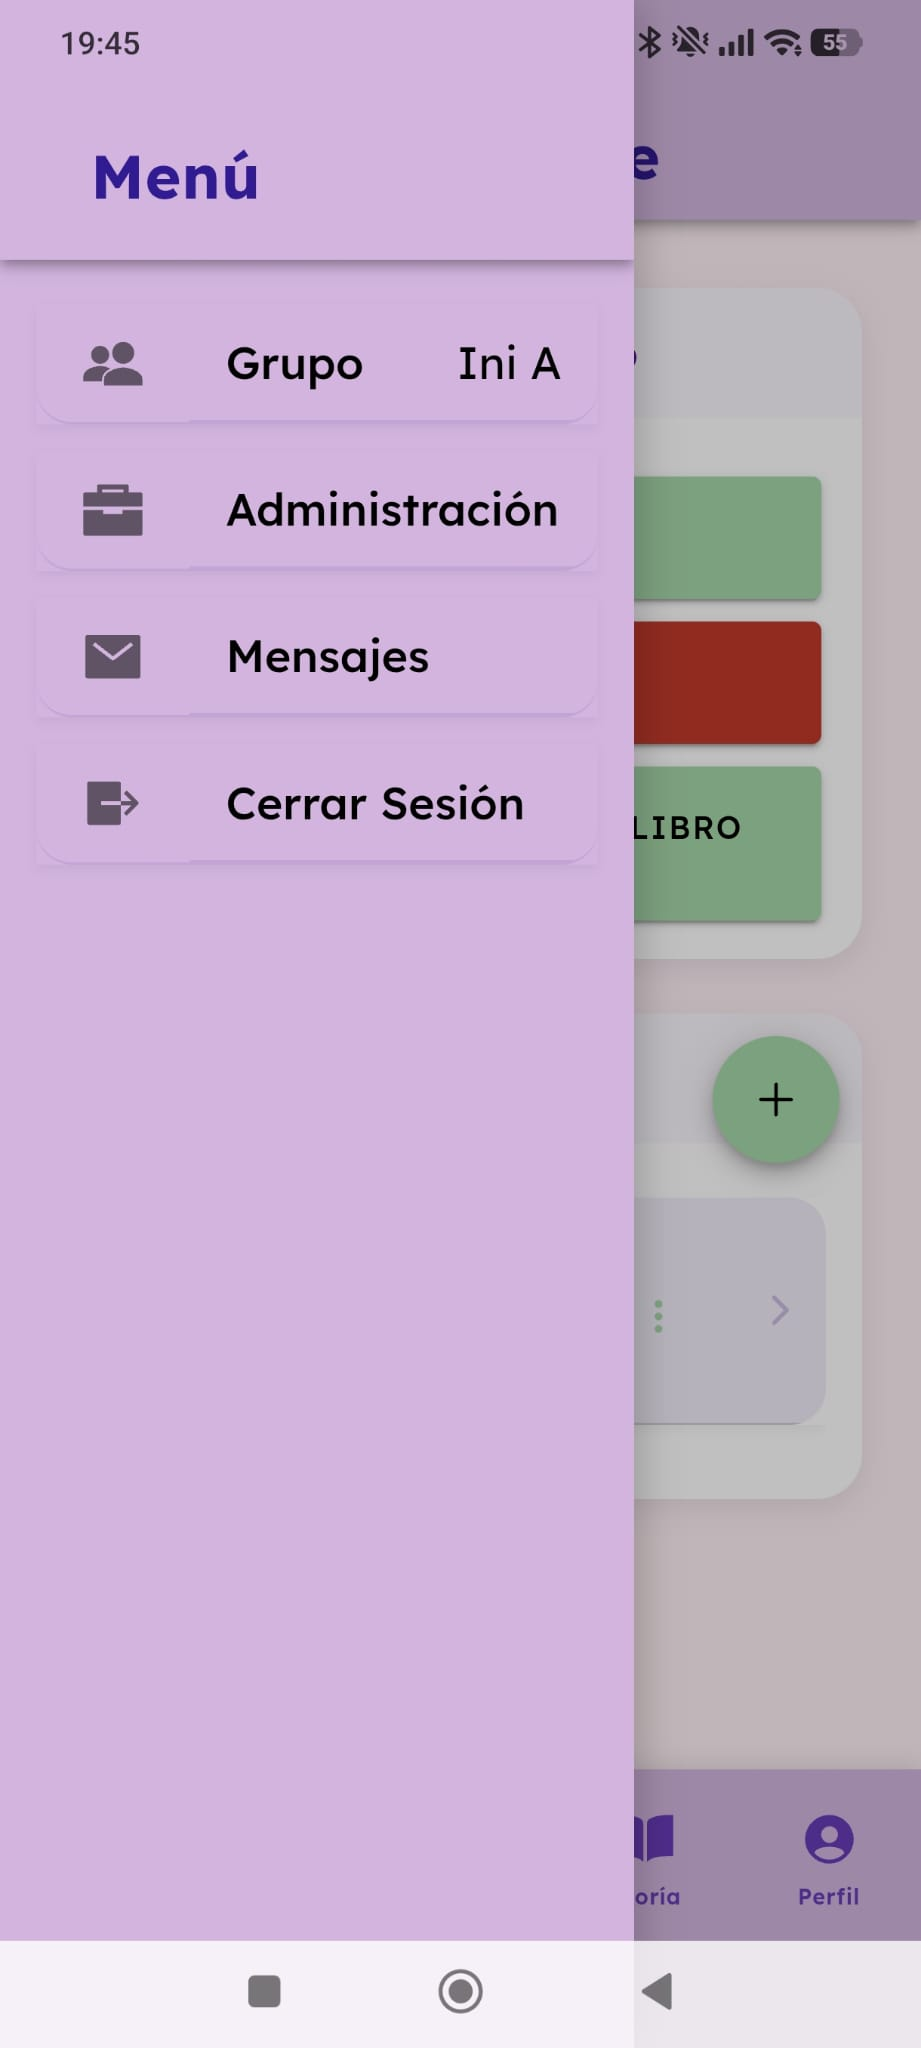
\includegraphics[width=0.3\textwidth]{Figuras/menus.png}
  \caption{Menú principal de navegación de la aplicación.}
  \label{fig:menus}
\end{figure}

\paragraph{Adaptaciones derivadas de la ejecución en Android}

Las modificaciones realizadas durante la implementación descrita anteriormente tienen una repercusión directa sobre la experiencia del usuario cuando la aplicación se ejecuta como software instalado.

Entre las mejoras más relevantes pueden destacarse las siguientes:

\begin{itemize}

    \item La utilización de \textit{safe areas} y la configuración de la barra de estado permiten evitar solapes con los elementos propios del sistema operativo, garantizando una correcta visualización de toda la interfaz.

    \item Los documentos PDF pasan a abrirse mediante el visor nativo del dispositivo, proporcionando una experiencia más estable y natural que la obtenida mediante un visor embebido.

    \item Determinados conjuntos de acciones se reorganizan automáticamente en pantallas reducidas, preservando la accesibilidad sin comprometer la claridad visual de la interfaz.

    \item Algunos componentes cuyo tamaño dependía del porcentaje de pantalla disponible han sido reajustados para mejorar su comportamiento en dispositivos móviles, especialmente en aquellos relacionados con la realización y edición de cuestionarios.

    \item La configuración de iconos y pantallas de carga mediante Android Studio permite que la aplicación se perciba como una aplicación nativa integrada en el sistema operativo.

\end{itemize}

Las Figuras~\ref{fig:ritmo_pc}, \ref{fig:ritmo}, \ref{fig:cuestionario_pc}, \ref{fig:cuestionario} y \ref{fig:splash_android} muestran algunos ejemplos representativos de estas adaptaciones.

\begin{figure}[H]
  \centering
  
\includegraphics[width=0.7\textwidth]{Figuras/Ritmo_pc.png}
  \caption{Vista de la rama de ritmo del profesor en la versión web.}
  \label{fig:ritmo_pc}
\end{figure}
\begin{figure}[H]
  \centering
  
\includegraphics[width=0.4\textwidth]{Figuras/Ritmo.png}
  \caption{Vista de la rama de ritmo del profesor en la versión android .}
  \label{fig:ritmo}
\end{figure}
\begin{figure}[H]
  \centering
  
\includegraphics[width=0.7\textwidth]{Figuras/cuestionario_pc.png}
  \caption{Vista de un cuestionario en la versión web (izquierda) y en Android (derecha).}
  \label{fig:cuestionario_pc}
\end{figure}
\begin{figure}[H]
  \centering

  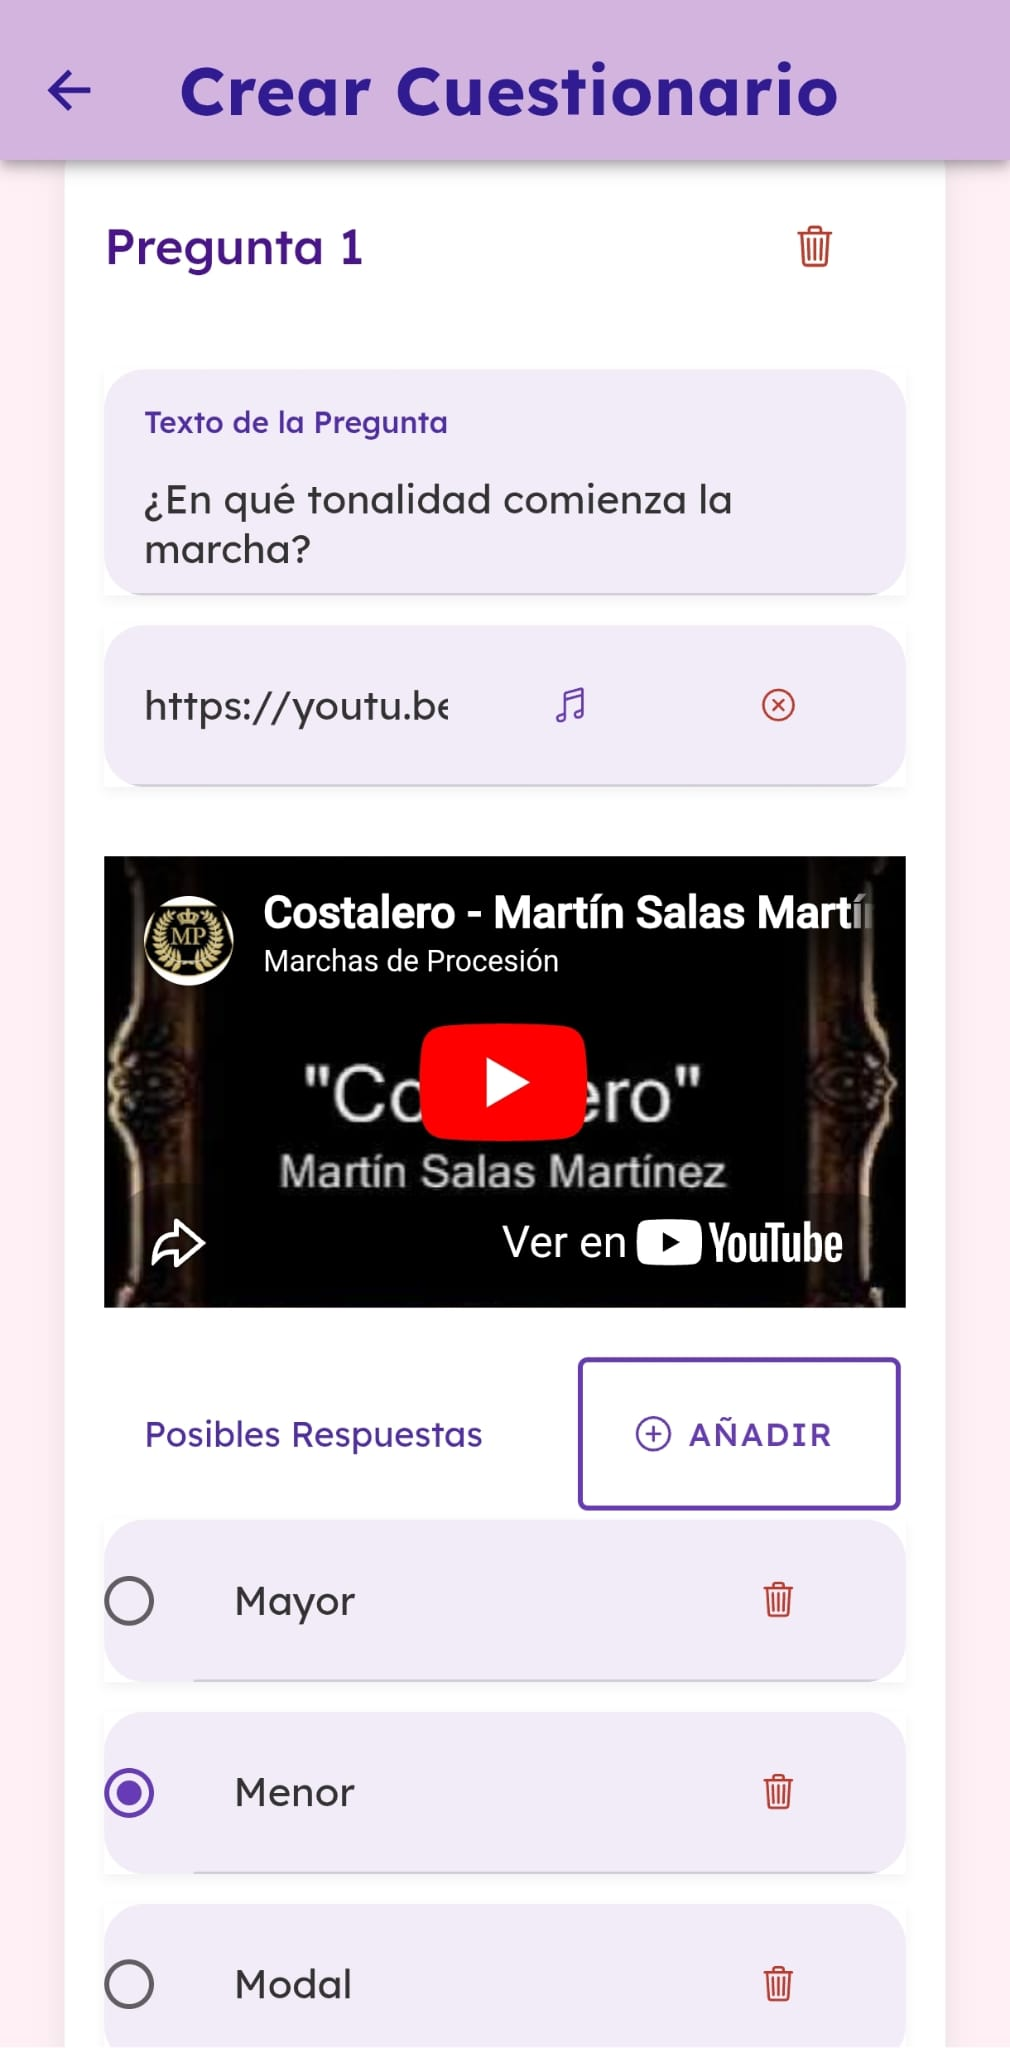
\includegraphics[width=0.4\textwidth]{Figuras/cuestionario.png}
  \caption{Vista de un cuestionario en la versión web (izquierda) y en Android (derecha).}
  \label{fig:cuestionario}
\end{figure}
\begin{figure}[H]
  \centering
  
\includegraphics[width=0.3\textwidth]{Figuras/splash.png}
  \caption{Icono y recursos gráficos utilizados por la aplicación Android.}
  \label{fig:splash_android}
\end{figure}

En conjunto, estas modificaciones permiten trasladar la aplicación al entorno móvil preservando la experiencia de uso definida originalmente y adaptándola a las características propias de este tipo de dispositivos.

\subsubsection{Testing}

La estrategia de pruebas del frontend mantiene el enfoque establecido durante el proyecto original, utilizando \textbf{Jasmine} como framework de pruebas unitarias y \textbf{Karma} como entorno de ejecución. Esta combinación continúa proporcionando un mecanismo eficaz para validar la lógica implementada en los componentes Angular y comprobar su correcta interacción con los distintos servicios de la aplicación.

Las nuevas funcionalidades incorporadas durante este complemento hacen necesario ampliar el conjunto de pruebas existentes, especialmente en aquellos componentes relacionados con la administración del sistema y con las nuevas operaciones de gestión de usuarios.

En este sentido, se ha prestado especial atención al componente encargado de la gestión de profesores, ya que incorpora nuevos flujos de revisión y eliminación definidos durante la ampliación funcional del sistema.

Las pruebas desarrolladas permiten verificar, entre otros aspectos:

\begin{itemize}
    \item La correcta inicialización del componente y la carga del listado de profesores.
    \item La comunicación con los servicios responsables de recuperar y eliminar usuarios.
    \item La aparición de confirmaciones antes de ejecutar operaciones irreversibles.
    \item La actualización del estado interno del componente tras una eliminación satisfactoria.
    \item El tratamiento adecuado de situaciones de error y la correspondiente notificación al usuario.
\end{itemize}

Para ello se mantiene el uso de \textit{spies} sobre los servicios de Angular y los distintos controladores proporcionados por Ionic, permitiendo aislar completamente el comportamiento del componente durante la ejecución de las pruebas.

Debido a la extensión del código generado, se presenta un pseudocódigo que resume el comportamiento validado por los distintos casos de prueba implementados.

\begin{Verbatim}[frame=single, fontsize=\small, xleftmargin=10pt, xrightmargin=10pt]

Inicializar entorno de pruebas

Crear mocks de dependencias:
  - ModalController
  - ToastController
  - AlertController
  - UsuarioService

Crear spies para métodos críticos:
  - dismiss()
  - create() y present() de alertas y toasts
  - getAllProfesores()
  - deleteUsuario()

Configurar TestBed con el componente y los mocks
Crear instancia del componente
Ejecutar ciclo inicial (ngOnInit)

TEST 1: Creación del componente

TEST 2: Carga inicial de profesores

TEST 3: Cierre del modal

TEST 4: Solicitud de eliminación

TEST 5: ID inválido

TEST 6: Confirmación de eliminación

TEST 7: Error en eliminación

TEST 8: Cancelación

\end{Verbatim}

Mediante este conjunto de pruebas se valida el correcto funcionamiento de uno de los principales módulos administrativos incorporados durante este complemento, garantizando que la evolución funcional del frontend mantiene el mismo nivel de calidad, estabilidad y fiabilidad alcanzado en la versión inicial del proyecto.

\subsection{Implementación del despliegue}
\label{sec:despliegue_impl}

La implementación de la solución se completa con el proceso de despliegue, que mantiene la infraestructura y metodología definidas en el Trabajo Fin de Grado. En lugar de replantear el flujo existente, este complemento amplía el proceso incorporando un nuevo escenario de despliegue orientado a la generación de una aplicación móvil Android, manteniendo en todo momento una única base de código para las versiones web y móvil.

De este modo, el despliegue web continúa realizándose mediante el flujo de integración y entrega continua previamente definido, mientras que la principal aportación de esta fase consiste en extender dicho proceso para permitir la construcción, empaquetado y validación de una aplicación Android instalada. Esta ampliación se apoya en la utilización conjunta de Capacitor y Android Studio, cuya integración con el frontend se ha descrito en la Sección~\ref{sec:frontend_impl}.

\subsubsection{Despliegue de la aplicación web}

Tal y como se detalló en el proyecto original, la aplicación mantiene un flujo de integración y entrega continua basado en \textbf{GitHub Actions}, utilizando \textbf{Render} para la publicación automática del backend, \textbf{GitHub Pages} para el despliegue del frontend web y \textbf{MongoDB Atlas} como servicio de base de datos en la nube.

Este mecanismo automatiza la ejecución de pruebas, la construcción de los artefactos y la publicación de nuevas versiones, garantizando la estabilidad del sistema y facilitando el mantenimiento continuo del proyecto. Dado que este procedimiento no ha experimentado modificaciones durante el desarrollo del presente complemento, no se reproduce nuevamente su descripción detallada, remitiéndose al lector al documento correspondiente al Trabajo Fin de Grado.

\subsubsection{Despliegue de la aplicación Android}

La principal ampliación realizada sobre el proceso de despliegue consiste en la posibilidad de distribuir la aplicación como una aplicación Android instalada, reutilizando íntegramente el frontend híbrido desarrollado con Ionic y Angular.

Esta capacidad constituye uno de los objetivos principales de este complemento, ya que permite trasladar la plataforma a dispositivos móviles sin necesidad de desarrollar una segunda aplicación específica para este entorno.

El proceso completo se apoya sobre dos herramientas principales:

\begin{itemize}
    \item \textbf{Capacitor}, encargado de encapsular la aplicación web y establecer la comunicación entre el código JavaScript y las funcionalidades nativas del sistema operativo.

    \item \textbf{Android Studio}, utilizado como entorno oficial para la compilación, depuración y generación del paquete instalable.
\end{itemize}

\paragraph{Generación del contenedor Android}

Capacitor permite transformar el frontend desarrollado con Ionic y Angular en un proyecto Android completamente funcional, manteniendo una única base de código para ambas plataformas.

El flujo seguido durante este proceso puede resumirse en las siguientes etapas:

\begin{enumerate}
    \item Compilación del frontend Angular en modo producción.
    \item Sincronización del proyecto mediante Capacitor.
    \item Generación automática de la estructura nativa Android.
    \item Apertura del proyecto generado en Android Studio.
\end{enumerate}

Este procedimiento permite reutilizar tanto la lógica de negocio como la interfaz de usuario previamente desarrolladas, garantizando la coherencia funcional entre la versión web y la versión móvil.

\paragraph{Construcción y validación}

Una vez generado el proyecto Android, Android Studio se emplea para completar las tareas específicas de la plataforma:

\begin{itemize}
    \item Gestión de dependencias nativas.
    \item Compilación del proyecto Android.
    \item Ejecución en emuladores y dispositivos físicos.
    \item Depuración de incidencias específicas del entorno móvil.
    \item Generación del paquete instalable (APK).
\end{itemize}

Además, este entorno permite configurar los recursos gráficos propios de Android, los permisos de la aplicación, el archivo de manifiesto y la pantalla de inicio, aspectos que complementan las adaptaciones del frontend descritas en la Sección~\ref{sec:frontend_impl}. Gracias a ello, la aplicación presenta una apariencia completamente integrada con el sistema operativo.

\paragraph{Generación del paquete instalable}

El proceso de despliegue culmina con la construcción de una \textbf{APK}, que constituye el artefacto final distribuible de la aplicación Android. Este paquete permite instalar directamente la aplicación en dispositivos físicos sin necesidad de recurrir a tiendas de aplicaciones, facilitando tanto las tareas de validación como futuras pruebas piloto en centros educativos.

\begin{figure}[H]
    \centering
    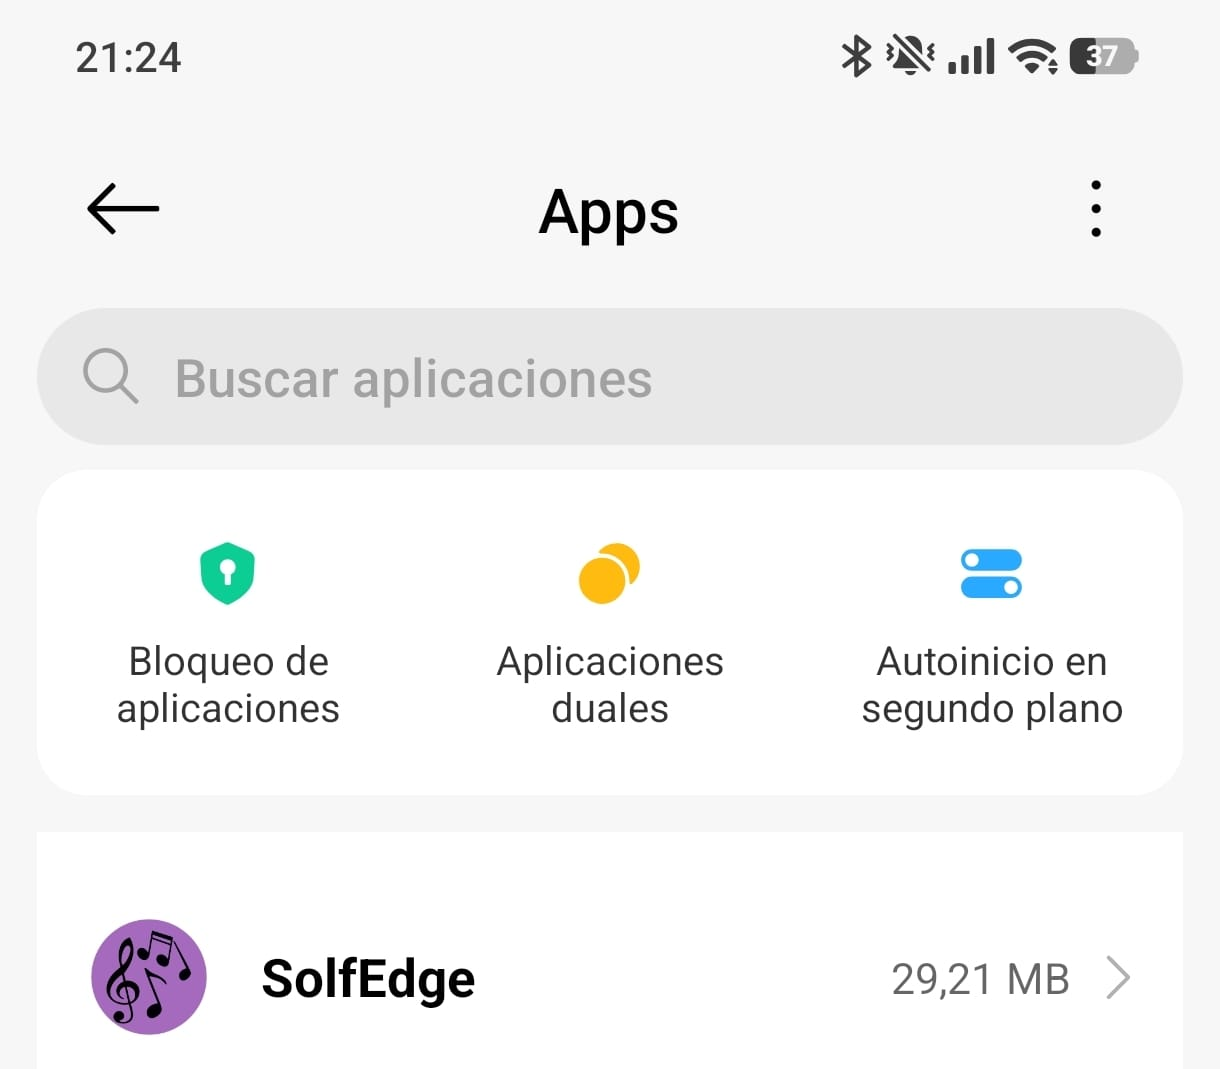
\includegraphics[width=0.7\textwidth]{Figuras/apk_install.png}
    \caption{Aplicación instalada en un dispositivo Android.}
    \label{fig:apk_install}
\end{figure}

\subsubsection{Valor aportado por el despliegue móvil}

La incorporación del despliegue Android representa una evolución significativa respecto a la versión desarrollada en el Trabajo Fin de Grado, ampliando el alcance de la plataforma sin modificar su arquitectura fundamental.

Entre las principales ventajas obtenidas pueden destacarse las siguientes:

\begin{itemize}
    \item Mejora la accesibilidad para alumnado y profesorado al permitir el uso de la aplicación desde dispositivos móviles.
    \item Facilita la utilización de la plataforma en contextos educativos reales, donde el teléfono móvil constituye uno de los principales dispositivos de acceso.
    \item Consolida la arquitectura híbrida adoptada durante el desarrollo del proyecto.
    \item Sienta las bases para futuras adaptaciones a otras plataformas móviles reutilizando la misma base de código.
\end{itemize}

Con esta ampliación finaliza la implementación técnica de la solución extendida, completando la evolución de la arquitectura desarrollada en el Trabajo Fin de Grado y proporcionando una plataforma preparada para abordar las cuestiones relativas a su futura implantación en entornos educativos reales, que se analizarán en el capítulo siguiente.

\chapter{Flujos de trabajo}
\label{chap:flujo}

Una vez descritas las principales decisiones de diseño e implementación de la solución extendida, este capítulo presenta el funcionamiento práctico de las nuevas funcionalidades incorporadas durante el desarrollo del complemento.

A diferencia del Trabajo Fin de Grado, donde se describía el funcionamiento general de la aplicación, en esta memoria el objetivo no es volver a recorrer todas las funcionalidades existentes, sino mostrar aquellas que representan la evolución realizada sobre la versión inicial del sistema.

Los flujos seleccionados corresponden a tres de las principales mejoras implementadas durante este complemento:

\begin{itemize}
    \item La eliminación de grupos desde la interfaz de administración.
    \item La importación masiva de usuarios y grupos mediante archivos CSV.
    \item La utilización de pistas generadas mediante inteligencia artificial durante la realización de cuestionarios.
\end{itemize}

Todas las capturas mostradas en este capítulo corresponden a la versión Android de la aplicación, demostrando que las funcionalidades implementadas mantienen el mismo comportamiento tanto en la versión web como en la aplicación instalada.

\section{Eliminación de un grupo}

La gestión de grupos constituye una de las tareas administrativas más habituales para el profesorado. Durante este complemento se ha ampliado esta funcionalidad incorporando una eliminación consistente de toda la información asociada al grupo, evitando que permanezcan tareas, cuestionarios o entregas huérfanas en el sistema.

La Figura~\ref{fig:flujo_eliminar_grupo} muestra el proceso de eliminación de un grupo desde la aplicación móvil. Tras entrar en la la opción de gestión de grupos de la administración del profesor, habrá una nuevaopción para eliminar el grupo.

\begin{figure}[H]
    \centering
    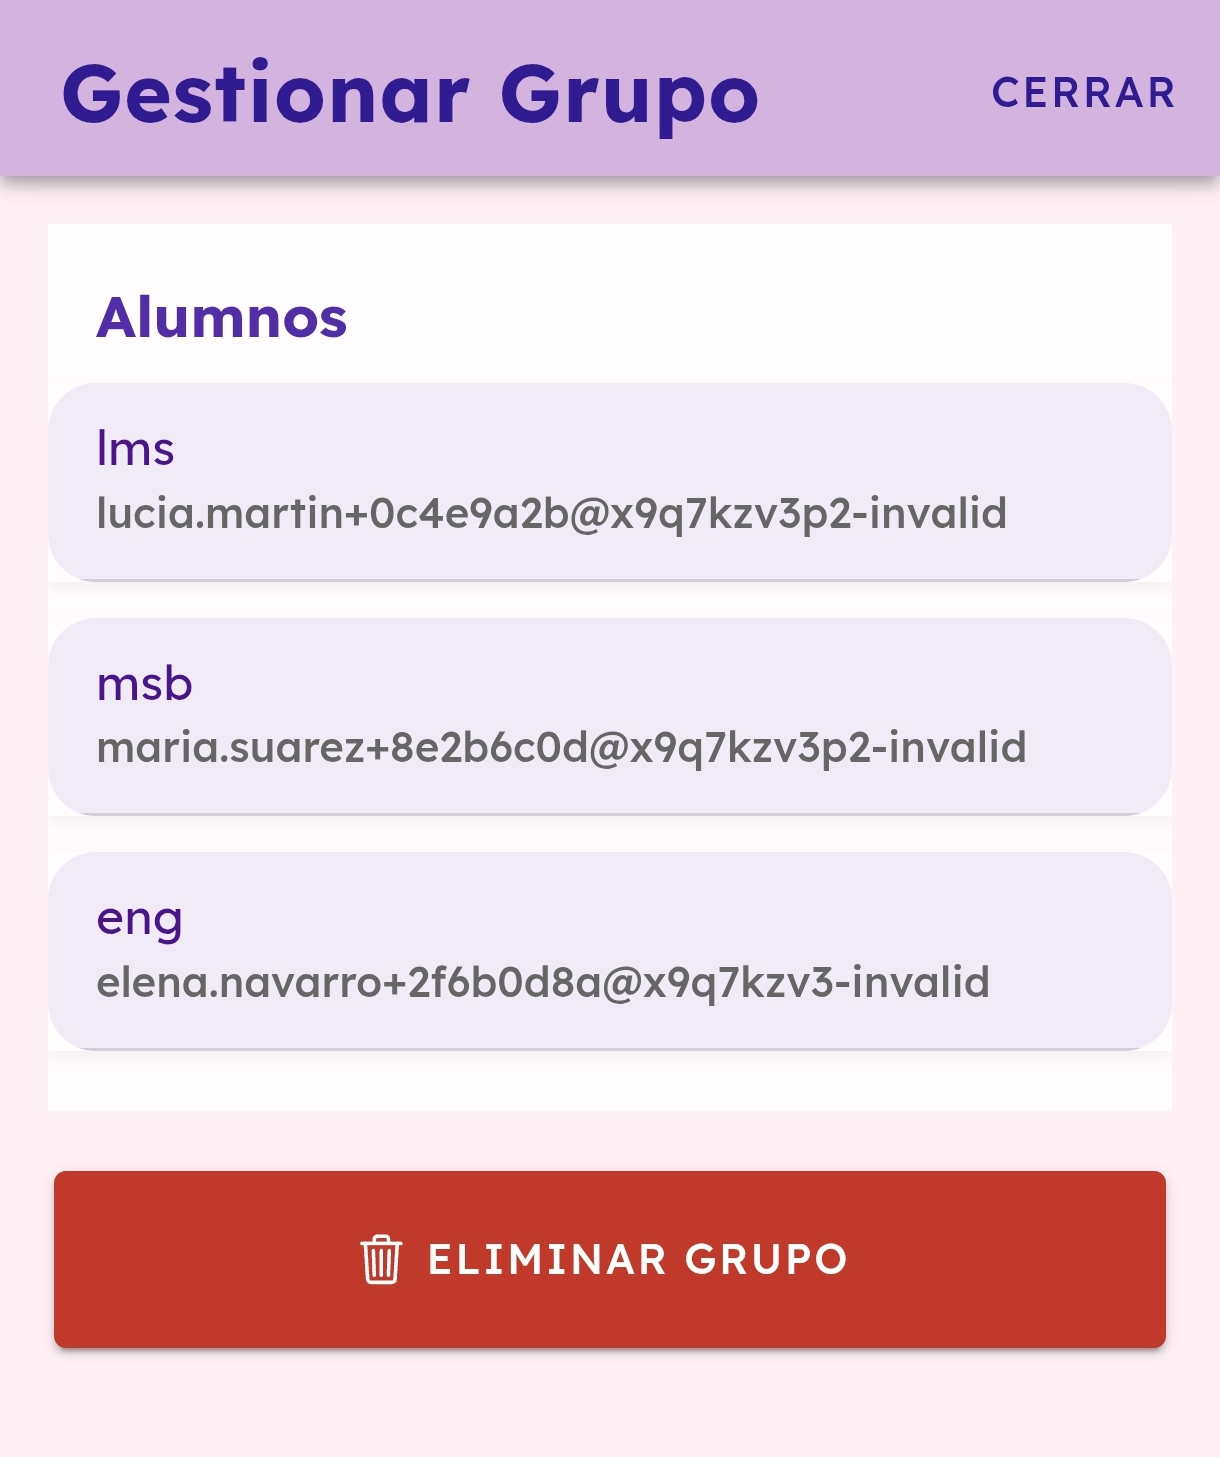
\includegraphics[width=0.32\textwidth]{Figuras/flujo_eliminar_grupo.png}
    \caption{Proceso de eliminación de un grupo desde la aplicación Android.}
    \label{fig:flujo_eliminar_grupo}
\end{figure}

Una vez confirmada la operación, el backend elimina de forma coordinada todas las entidades relacionadas con el grupo, preservando la integridad de la información almacenada en la base de datos.

\section{Importación masiva mediante archivos CSV}

Otra de las funcionalidades incorporadas durante este complemento permite automatizar la creación de usuarios y grupos a partir de un archivo CSV, reduciendo considerablemente el trabajo administrativo necesario al inicio de cada curso académico.

La Figura~\ref{fig:flujo_csv} muestra la interfaz desde la que el profesorado puede seleccionar el archivo correspondiente e iniciar el proceso de importación \cite{OWASPFileUpload}.

\begin{figure}[H]
    \centering
    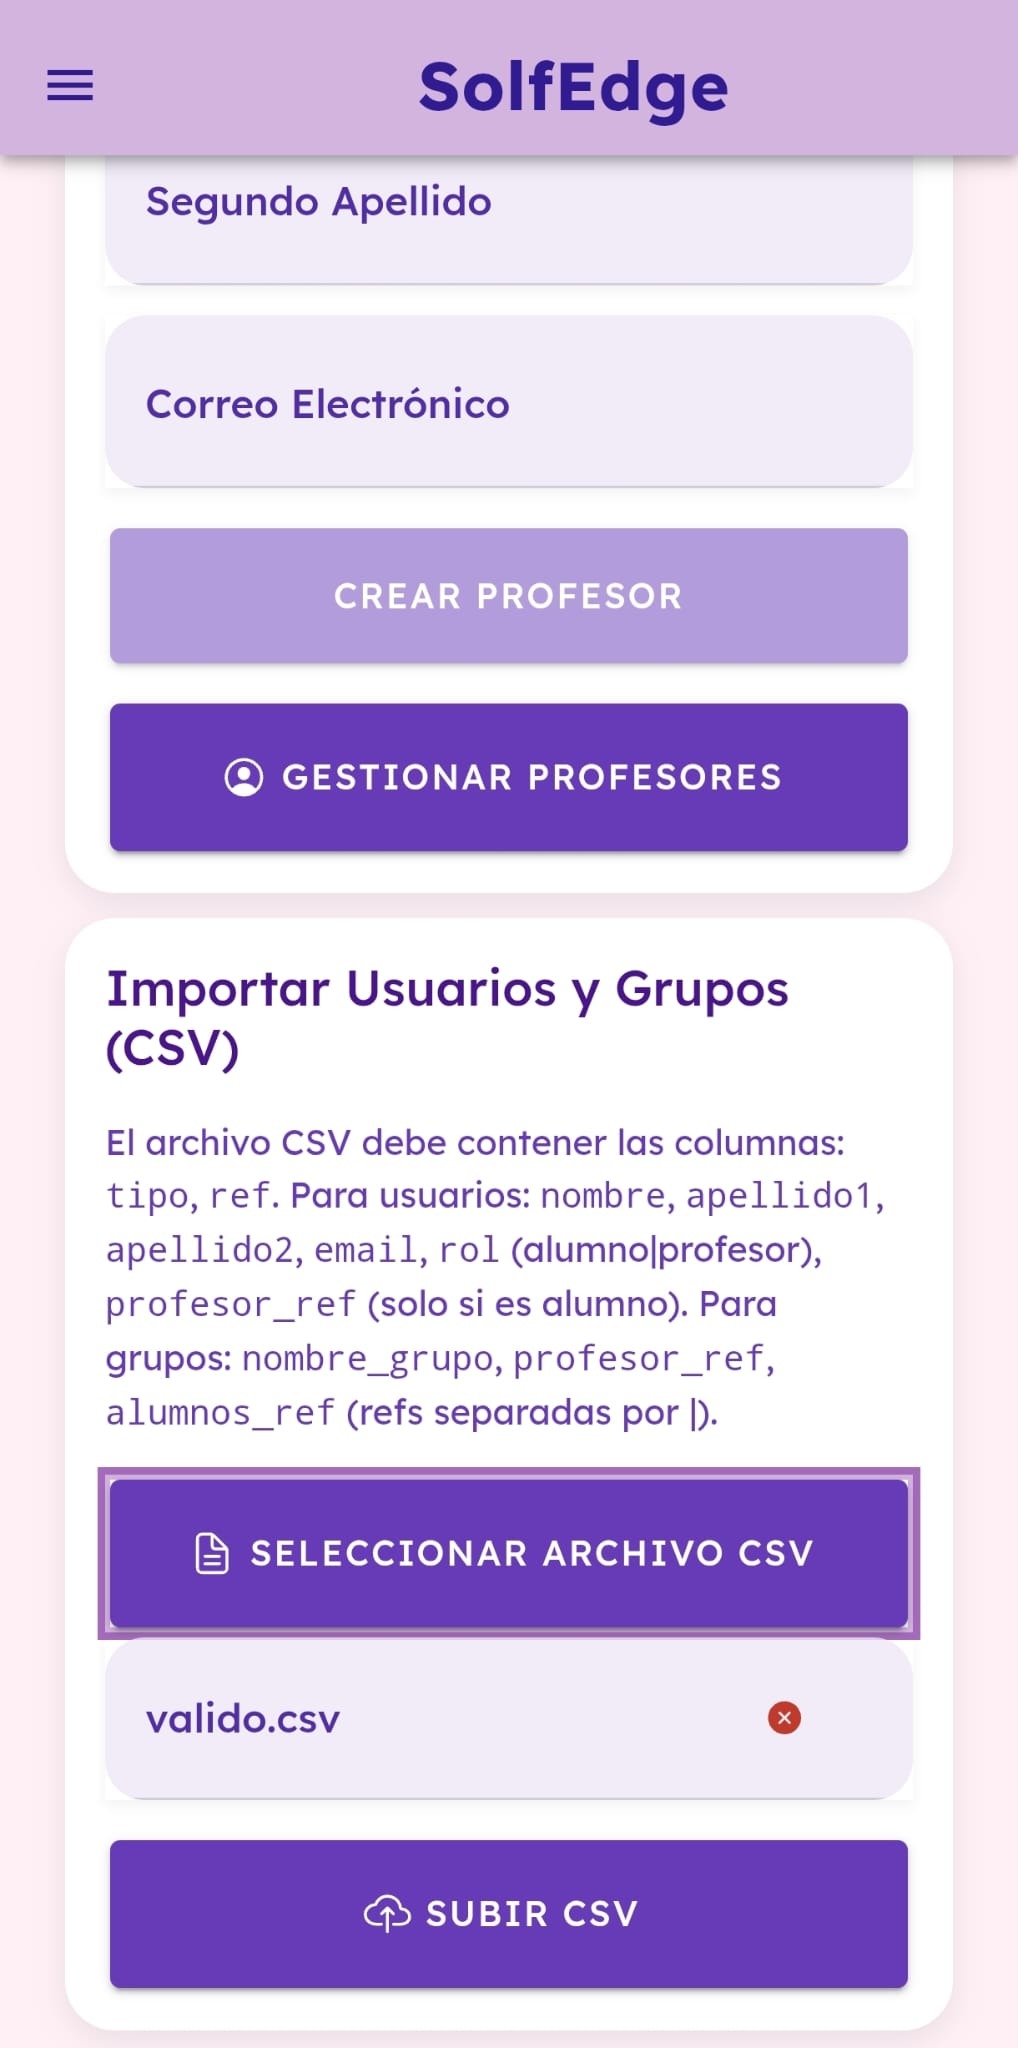
\includegraphics[width=0.32\textwidth]{Figuras/flujo_importacion_csv.png}
    \caption{Importación masiva de usuarios y grupos mediante un archivo CSV.}
    \label{fig:flujo_csv}
\end{figure}

Una vez seleccionado el archivo, el backend realiza automáticamente todas las validaciones descritas en el capítulo anterior. Únicamente cuando la información es consistente se inicia la creación de usuarios y grupos, garantizando que el sistema nunca alcance estados parciales o inconsistentes.

\section{Resolución de cuestionarios con asistencia mediante inteligencia artificial}

La tercera funcionalidad incorporada corresponde a la generación automática de pistas para preguntas de cuestionarios utilizando un modelo de inteligencia artificial integrado mediante la API de Groq.

Durante la realización de un cuestionario, el alumnado puede solicitar una pista cuando encuentre dificultades para responder una pregunta. El sistema genera entonces una ayuda contextual relacionada con el contenido de la cuestión, evitando revelar directamente la respuesta correcta y manteniendo el carácter formativo de la actividad.

La Figura~\ref{fig:flujo_pistas} muestra un ejemplo de utilización de esta funcionalidad desde la aplicación Android.

\begin{figure}[H]
    \centering
    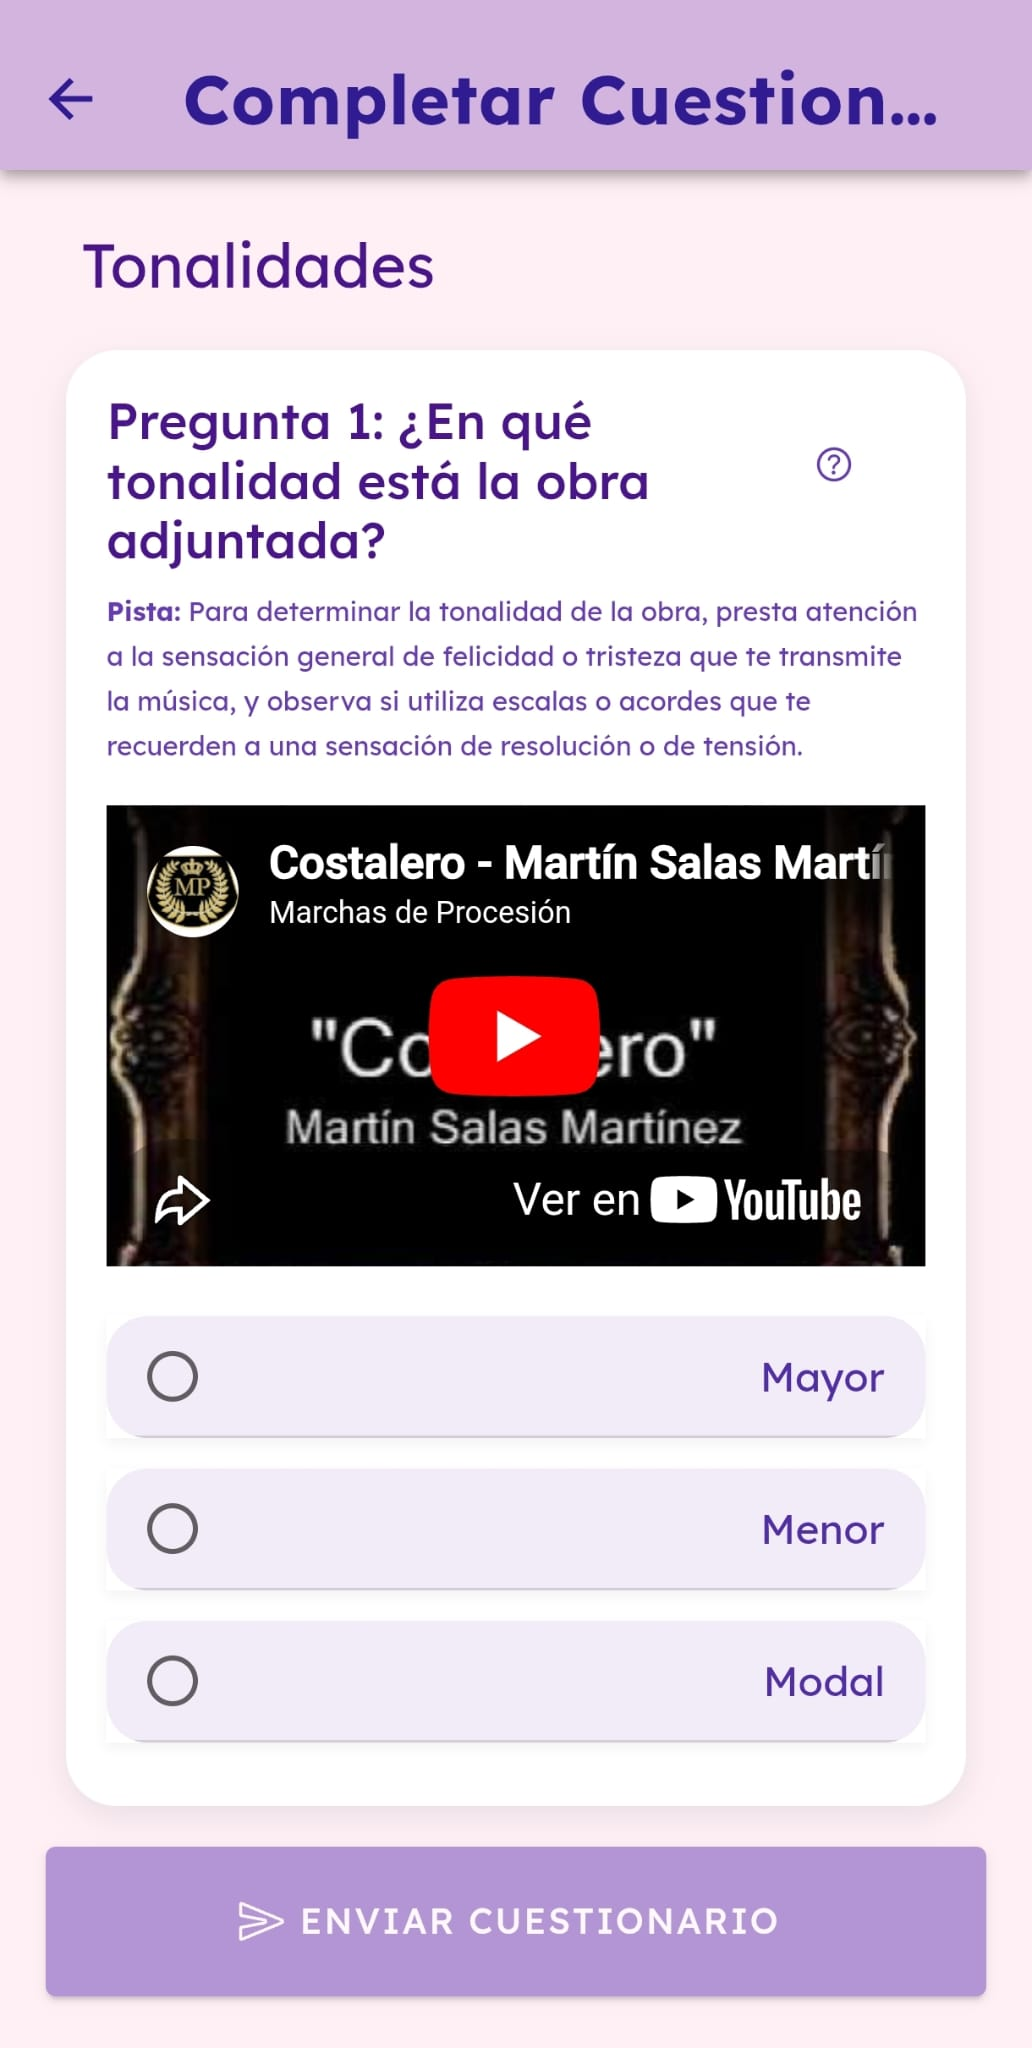
\includegraphics[width=0.32\textwidth]{Figuras/flujo_pista_ia.png}
    \caption{Solicitud de una pista generada mediante inteligencia artificial durante la realización de un cuestionario.}
    \label{fig:flujo_pistas}
\end{figure}

La petición realizada por el usuario es procesada por el backend, que construye el \textit{prompt} correspondiente y consulta el servicio de Groq. La respuesta obtenida se devuelve posteriormente al dispositivo móvil en forma de una pista breve que ayuda al alumnado a razonar la respuesta sin proporcionarla explícitamente.

Este flujo ilustra la integración práctica de la inteligencia artificial dentro de la aplicación y representa una de las principales aportaciones funcionales realizadas durante el presente complemento.

\chapter{Plan de implantación}
\label{chap:implantacion}

El presente capítulo describe un plan integral para la implantación progresiva de la solución desarrollada en un entorno educativo real. Aunque durante el desarrollo de este proyecto no se ha llevado a cabo una implantación completa siguiendo dicho plan, sí se ha realizado una validación preliminar en un centro educativo, mostrando el funcionamiento general de la aplicación y recogiendo observaciones directas del profesorado. Esta experiencia, descrita en el apartado~\ref{sec:validacion_preliminar}, ha permitido detectar mejoras relevantes y refuerza la necesidad de contar con un plan estructurado que guíe una futura implantación realista.

El objetivo de este plan no es documentar un proceso ya ejecutado, sino establecer un marco estratégico, técnico y organizativo que permita, en un escenario real, desplegar la aplicación de forma segura, estable, escalable y sostenible, contemplando tanto los aspectos tecnológicos como los humanos y organizativos implicados. Este enfoque resulta coherente con la evolución funcional y tecnológica presentada en los sección~\ref{sec:arquitectura_implementacion}.

Además, cabe destacar que las decisiones técnicas adoptadas a lo largo del proyecto han favorecido de manera significativa su adaptación a un contexto real de implantación. Las tecnologías seleccionadas, aunque en su configuración actual priorizan el uso de recursos gratuitos y presentan limitaciones para un entorno productivo, ofrecen planes de escalado superiores o permiten una migración sencilla hacia infraestructuras de pago, sin necesidad de reestructurar la arquitectura del sistema. Asimismo, aunque se han identificado determinados aspectos susceptibles de mejora en materia de seguridad, estos quedan documentados como líneas de evolución futura, manteniendo la versión actual del sistema suficientemente preparada para asumir dichos cambios de forma progresiva y controlada.
\section{Objetivos del plan de implantación}
\label{sec:objetivos_implantacion}

La implantación de un sistema informático en un entorno educativo requiere una planificación cuidadosa que tenga en cuenta múltiples factores. En este contexto, el plan de implantación persigue los siguientes objetivos principales:

\begin{itemize}
    \item Garantizar una transición progresiva desde el entorno de desarrollo hacia un entorno productivo real, minimizando interrupciones en la actividad docente.
    \item Asegurar la estabilidad técnica del sistema, su disponibilidad continua y la integridad de los datos almacenados, en coherencia con los principios arquitectónicos definidos en el apartado~\ref{sec:tecnologias_ext} y en la versión inicial.
    \item Facilitar la adopción de la herramienta por parte del profesorado y el alumnado, reduciendo la resistencia al cambio mediante interfaces intuitivas y procesos alineados con la práctica educativa real.
    \item Proteger los datos personales gestionados por el sistema, especialmente aquellos relativos a menores, cumpliendo con la normativa vigente en materia de protección de datos \cite{RGPD2016}.
    \item Definir un marco de mantenimiento, soporte y evolución que garantice la sostenibilidad del proyecto a medio y largo plazo.
\end{itemize}

Estos objetivos sitúan la implantación como una fase crítica dentro del ciclo de vida del sistema, en la que convergen aspectos técnicos, organizativos, legales y pedagógicos, complementando el proceso de desarrollo descrito en los capítulos anteriores.

\section{Contexto de implantación en centros educativos}
\label{sec:contexto_implantacion}

La aplicación ha sido concebida para su uso en centros educativos dedicados a la enseñanza musical, tales como conservatorios profesionales, escuelas municipales de música o academias privadas. Este enfoque se deriva directamente del análisis funcional y pedagógico realizado en el proyecto original y sintetizado en el capítulo~\ref{chap:contexto}.

Estos entornos presentan una serie de características comunes que condicionan el proceso de implantación:

\begin{itemize}
    \item Existencia de múltiples perfiles de usuario con roles claramente diferenciados, tal y como se definió en la especificación funcional del sistema (apartado~\ref{sec:especificacion_formal_extendida}).
    \item Gestión simultánea de múltiples grupos, niveles académicos y asignaturas.
    \item Necesidad de acceso desde distintos dispositivos y ubicaciones, lo que refuerza la importancia de la portabilidad móvil abordada en el apartado~\ref{sec:frontend_impl}.
    \item Infraestructuras tecnológicas heterogéneas y, en muchos casos, limitadas.
\end{itemize}

Además, estos centros suelen contar con sistemas propios de gestión académica, lo que introduce la necesidad de contemplar procesos de migración e integración de datos. En este contexto, la implantación del sistema debe realizarse de forma progresiva y flexible, adaptándose a las particularidades organizativas y tecnológicas de cada institución.


\section{Estrategia de implantación progresiva}
\label{sec:estrategia_implantacion}

La implantación del sistema se estructura como un proceso progresivo, planificado en fases claramente diferenciadas, con el objetivo de reducir riesgos técnicos y organizativos, facilitar la adaptación de los usuarios y garantizar la estabilidad del servicio antes de su adopción completa.

La implantación se ejecutará en tres fases sucesivas, cada una con objetivos, tareas y criterios de validación claramente definidos.

\subsection{Fase 1: Despliegue piloto}

Durante esta primera fase, el sistema se implantará en un entorno real pero controlado, con un número reducido de usuarios. Esta fase se desarrollará durante un periodo estimado de \textbf{cuatro a seis semanas}.

El despliegue piloto se realizará con:
\begin{itemize}
    \item Un único profesor voluntario.
    \item Uno o dos grupos reducidos de alumnos.
\end{itemize}

Las acciones concretas que se llevarán a cabo son:

\begin{enumerate}
    \item Despliegue del backend y frontend en el entorno productivo seleccionado.
    \item Configuración inicial del sistema y validación de la infraestructura.
    \item Creación controlada de usuarios reales y verificación de accesos por rol.
    \item Importación de datos académicos mediante los mecanismos desarrollados.
    \item Uso cotidiano del sistema en actividades docentes reales, siguiendo la operativa definida en los casos de uso y requisitos funcionales descritos en el documento.
    \item Registro sistemático de incidencias técnicas y funcionales, así como recopilación de feedback del profesorado.
\end{enumerate}

Los objetivos verificables de esta fase son:

\begin{itemize}
    \item Validar el correcto funcionamiento del sistema bajo condiciones reales.
    \item Identificar errores no detectados en el entorno de desarrollo.
    \item Evaluar la estabilidad general de la aplicación (backend, frontend y comunicaciones).
    \item Recoger feedback directo del profesorado y alumnado para priorizar ajustes.
\end{itemize}

Al finalizar esta fase se elaborará un \textbf{informe técnico de validación}, que servirá como base para introducir ajustes correctivos antes de avanzar a la siguiente etapa.

\subsection{Fase 2: Despliegue parcial}

Una vez validados los resultados del piloto, se procederá a un despliegue parcial ampliado durante un periodo aproximado de \textbf{dos a tres meses}.

En esta fase, el sistema se extenderá a:

\begin{itemize}
    \item Varios profesores.
    \item Múltiples grupos de distintos niveles dentro del mismo centro.
\end{itemize}

Las acciones planificadas son:

\begin{enumerate}
    \item Ampliación progresiva del número de usuarios y grupos activos.
    \item Verificación de rendimiento bajo mayor carga (usuarios concurrentes, accesos a materiales, entregas y cuestionarios).
    \item Ajuste de los procesos administrativos internos del centro relacionados con altas/bajas y gestión de grupos.
    \item Monitorización intensiva del consumo de recursos y revisión de logs para detectar cuellos de botella.
    \item Consolidación de procedimientos de soporte: canal de incidencias, prioridades y tiempos de respuesta.
\end{enumerate}

Los objetivos principales son:

\begin{itemize}
    \item Validar la escalabilidad del sistema.
    \item Detectar cuellos de botella de rendimiento o límites de infraestructura.
    \item Refinar la gestión de recursos multimedia y archivos.
    \item Ajustar los flujos reales de trabajo del profesorado, reduciendo fricciones.
\end{itemize}

\subsection{Fase 3: Despliegue completo}

Tras completar con éxito la fase parcial, se ejecutará el despliegue completo en el centro educativo, integrando el sistema como herramienta habitual.

Las acciones serán:

\begin{enumerate}
    \item Alta y verificación de todos los profesores participantes.
    \item Migración completa de grupos y datos académicos.
    \item Activación del servicio como sistema operativo estándar del centro para las funcionalidades definidas.
    \item Activación completa de los mecanismos de monitorización y respaldo.
\end{enumerate}

Esta fase marca la transición del sistema a \textbf{herramienta central de apoyo docente}, integrándose en la operativa diaria del centro.

\section{Migración tecnológica hacia un entorno productivo}
\label{sec:migracion_tecnologica}

La migración tecnológica constituye un eje central del plan de implantación, cuyo objetivo es transformar la infraestructura académica y experimental en una plataforma productiva, escalable y robusta. Este proceso se apoya en la arquitectura modular descrita en el apartado~\ref{sec:tecnologias_ext}, que permite sustituir piezas de infraestructura minimizando el impacto sobre el código.

\subsection{Justificación de la migración}

Durante el desarrollo del proyecto se priorizó el uso de tecnologías gratuitas por motivos académicos. En un escenario real de operación continuada, esta infraestructura puede resultar limitada en términos de disponibilidad, escalado, monitorización y soporte. Por tanto, se realizará una migración controlada hacia servicios cloud profesionales que permitan:

\begin{itemize}
    \item Escalado automático bajo picos de carga.
    \item Mayor disponibilidad y redundancia.
    \item Monitorización avanzada y alertas.
    \item Soporte técnico profesional y SLAs.
\end{itemize}

\subsection{Migración del backend y frontend a Microsoft Azure}
\label{sec:migracion_azure}

La migración de los servicios web hacia un entorno productivo se apoyará en la plataforma \textbf{Microsoft Azure} \cite{azure_docs}, aprovechando su ecosistema cloud maduro, su integración con herramientas de desarrollo modernas y su capacidad para proporcionar una infraestructura altamente escalable, resiliente y monitorizable.

La arquitectura definida en el apartado~\ref{sec:tecnologias_ext} facilita este proceso, ya que el sistema presenta una clara separación entre frontend, backend y base de datos, permitiendo una transición progresiva sin necesidad de modificar la lógica de la aplicación. En este contexto, Azure App Service \cite{azure_app_service_docs} se utilizará como plataforma unificada tanto para el despliegue del backend como del frontend, garantizando una gestión homogénea de los recursos y un control centralizado del entorno productivo.

\subsubsection{Azure App Service como plataforma de ejecución}

Azure App Service proporciona un entorno gestionado para la ejecución de aplicaciones web, APIs REST y servicios backend, abstrayendo la complejidad asociada a la gestión directa de servidores, redes, balanceo de carga y sistemas operativos. Este modelo permite centrar los esfuerzos en el desarrollo funcional, delegando en la plataforma cloud la responsabilidad del escalado, la disponibilidad y la seguridad perimetral.

Desde el punto de vista técnico, Azure App Service ofrece las siguientes capacidades clave:

\begin{itemize}
    \item \textbf{Escalado vertical}: Permite aumentar dinámicamente la capacidad de cómputo asignada a la aplicación (CPU, memoria RAM y rendimiento de disco), adaptando el entorno de ejecución a mayores cargas sin modificar la arquitectura del sistema.
    
    \item \textbf{Escalado horizontal}: Posibilita la ejecución simultánea de múltiples instancias de la aplicación, distribuyendo la carga de peticiones entrantes mediante balanceo automático. Este mecanismo resulta especialmente relevante en escenarios con alta concurrencia, ya que permite absorber incrementos súbitos de tráfico manteniendo tiempos de respuesta estables.
    
    \item \textbf{Gestión automática de infraestructura}: Azure se encarga del aprovisionamiento, monitorización y recuperación ante fallos de las instancias, garantizando una elevada disponibilidad del servicio sin intervención manual.
    
    \item \textbf{Integración nativa con CI/CD}: Azure App Service se integra de forma directa con GitHub Actions, facilitando la automatización completa del flujo de despliegue, tal y como se describe en el la sección \ref{sec:despliegue_impl}. En consecuencia, todas las operaciones de la migración quedarán integradas de forma automática con tan solo unas líneas en el archivo \texttt{.YML} que lee GitHub Actions.
\end{itemize}

Este conjunto de características convierte a Azure App Service en una plataforma idónea para albergar tanto el backend Node.js como el frontend Angular/Ionic, permitiendo un despliegue coherente, altamente disponible y preparado para un crecimiento progresivo del número de usuarios.

\subsubsection{Arquitectura de despliegue propuesta}

La arquitectura de despliegue en Azure se estructura en los siguientes componentes principales:

\begin{itemize}
    \item \textbf{Backend}: Desplegado en un recurso Azure App Service configurado para Node.js, con políticas de escalado automático basadas en consumo de CPU, memoria y volumen de peticiones HTTP.
    
    \item \textbf{Frontend}: Desplegado también sobre Azure App Service, sirviendo los recursos estáticos generados por el proceso de construcción de Angular/Ionic, permitiendo igualmente escalado horizontal bajo alta carga.
    
    \item \textbf{Servicios auxiliares}: Almacenamiento de variables de entorno, gestión segura de secretos y configuración centralizada mediante Azure Key Vault \cite{azure_key_vault_docs}.
\end{itemize}

Esta disposición garantiza un comportamiento homogéneo en ambos extremos de la aplicación y facilita la administración global del sistema desde un único entorno cloud.

\subsubsection{Proceso de migración}

La migración de los servicios web se ejecutará siguiendo un proceso estructurado en cuatro fases claramente definidas:

\begin{enumerate}
    \item \textbf{Creación de infraestructura base en Azure}: Provisión de recursos App Service para backend y frontend, definición de grupos de recursos, configuración de redes virtuales, reglas de firewall y establecimiento de variables de entorno seguras.
    
    \item \textbf{Configuración de despliegue automatizado}: Adaptación del pipeline de integración y despliegue continuo descrito en el proyecto original, modificando exclusivamente los endpoints de despliegue para apuntar a Azure, manteniendo intacta la lógica de CI/CD.
    
    \item \textbf{Despliegue inicial en Azure y validación funcional}: Verificación exhaustiva del correcto funcionamiento del sistema, comprobando procesos de autenticación, acceso a la base de datos, ejecución de operaciones CRUD principales y respuesta bajo carga simulada.
    
    \item \textbf{Cambio controlado de tráfico}: Una vez validado el entorno productivo, redirección progresiva del tráfico desde el entorno anterior hacia Azure, minimizando interrupciones del servicio.
\end{enumerate}

Este procedimiento permite garantizar una transición segura, reversible y con impacto mínimo sobre los usuarios finales.

\subsubsection{Pipeline de despliegue automatizado}
\label{sec:pipeline_azure}

El objetivo principal de esta migración es que el cambio afecte únicamente al flujo de despliegue, sin introducir modificaciones en la lógica del sistema. La estructura modular del proyecto y el uso de contenedores Docker en la fase de implantación \cite{docker_docs} permiten desacoplar completamente la ejecución de la aplicación del entorno subyacente, lo que facilita la transición desde un despliegue local hacia una infraestructura en la nube sin necesidad de reescritura del código.

La aplicación desarrollada, se despliega en la plataforma Microsoft Azure utilizando el servicio \textit{Azure App Service for Containers}, que permite ejecutar contenedores Docker de forma gestionada, escalable y altamente disponible. Como registro privado se emplea \textit{Azure Container Registry} (ACR) \cite{azure_container_registry_docs}, que actúa como repositorio centralizado de imágenes Docker.

Para la correcta ejecución del pipeline de despliegue es necesario realizar previamente una serie de configuraciones en Azure, que se detallan a continuación.

\paragraph{Configuración previa en Azure}

Antes de poder automatizar el despliegue, es imprescindible preparar la infraestructura mínima necesaria en la plataforma Azure:

\begin{itemize}
    \item \textbf{Creación del grupo de recursos}: Se define un grupo de recursos (por ejemplo, \texttt{RCPMA}) como convención de nomenclatura para agrupar todos los servicios asociados. Este identificador se emplea a modo ilustrativo y puede adaptarse al centro que realice la implantación.
    
    \item \textbf{Creación del Azure Container Registry (ACR):} Se crea un registro privado de contenedores donde se almacenarán las imágenes Docker del frontend y backend. Este registro permite la gestión segura, versionada y centralizada de las imágenes, facilitando su despliegue automatizado.
    
    \item \textbf{Creación de las Web Apps para contenedores:} Se crean dos instancias independientes de \textit{Azure App Service for Containers} (sobre sistema Linux), una destinada al frontend (\texttt{solfedge-frontend}) y otra al backend (\texttt{solfedge-backend}). Estas aplicaciones se configuran para obtener sus imágenes desde el ACR.
    
    \item \textbf{Creación del Service Principal:} Se genera una identidad de servicio con permisos suficientes para autenticarse contra Azure, subir imágenes al ACR y modificar la configuración de las Web Apps. Las credenciales asociadas a este Service Principal se almacenan como secretos seguros en GitHub Actions.
\end{itemize}

Esta configuración inicial permite disponer de un entorno completamente preparado para recibir despliegues automáticos desde el repositorio de código.

\paragraph{Flujo general de despliegue}

El proceso completo de despliegue automatizado se integra dentro del pipeline CI/CD del proyecto, ejecutándose de forma automática cada vez que se realiza un \textit{push} sobre la rama principal del repositorio. Dicho flujo consta de las siguientes fases:

\begin{enumerate}
    \item Descarga del código fuente desde el repositorio.
    \item Autenticación segura contra Azure mediante credenciales almacenadas en GitHub Secrets.
    \item Construcción de las imágenes Docker correspondientes al frontend y backend.
    \item Publicación de dichas imágenes en el Azure Container Registry.
    \item Actualización automática de las Web Apps para que utilicen la nueva versión de las imágenes.
\end{enumerate}

Este enfoque garantiza un despliegue reproducible, trazable y consistente, eliminando la intervención manual y reduciendo drásticamente la probabilidad de errores humanos.

\paragraph{Pipeline de despliegue}

A continuación se muestra un pipeline orientativo que ilustra el proceso completo de construcción, publicación y despliegue automático del sistema en Azure. Este pipeline se apoya en las fases previas de construcción y testeo ya descritas, adaptando únicamente la etapa final de despliegue al entorno cloud.
\newpage
\begin{Verbatim}[frame=single, fontsize=\small]
push-and-deploy-frontend:
  if: github.ref == 'refs/heads/main'
  runs-on: ubuntu-latest
  needs: build-frontend

  steps:
    - name: Checkout code
      uses: actions/checkout@v3

    - name: Login to Azure CLI
      uses: azure/login@v1
      with:
        creds: ${{ secrets.AZURE_CREDENTIALS }}

    - name: Download artifacts
      uses: actions/download-artifact@v4
      with: 
        name: www
        path: ./www

    - name: Build and push frontend Docker image to ACR
      run: |
        IMAGE_NAME=repodocker.azurecr.io/solfedge-frontend:
        ${{ github.run_number }}
        docker build -t $IMAGE_NAME ./frontend
        echo ${{ secrets.AZURE_PASSWORD }} | docker login \
        repodocker.azurecr.io -u ${{ secrets.AZURE_USERNAME }} \
        --password-stdin
        docker push $IMAGE_NAME

    - name: Deploy frontend to Azure Web App for Containers
      run: |
        IMAGE_NAME=repodocker.azurecr.io/solfedge-frontend:
        ${{ github.run_number }}
        az webapp config container set \
          --docker-custom-image-name $IMAGE_NAME \
          --docker-registry-server-password ${{ secrets.AZURE_PASSWORD }} \
          --docker-registry-server-url https://repodocker.azurecr.io \
          --docker-registry-server-user ${{ secrets.AZURE_USERNAME }} \
          --name solfedge-frontend \
          --resource-group RCPMA


push-and-deploy-backend:
  if: github.ref == 'refs/heads/main'
  runs-on: ubuntu-latest
  needs: build-backend

  steps:
    - name: Checkout code
      uses: actions/checkout@v3

    - name: Login to Azure CLI
      uses: azure/login@v1
      with:
        creds: ${{ secrets.AZURE_CREDENTIALS }}

    - name: Build and push backend Docker image to ACR
      run: |
        IMAGE_NAME=repodocker.azurecr.io/solfedge-backend:
        ${{ github.run_number }}
        docker build -t $IMAGE_NAME ./backend
        echo ${{ secrets.AZURE_PASSWORD }} | docker login \
        repodocker.azurecr.io -u ${{ secrets.AZURE_USERNAME }} \
        --password-stdin
        docker push $IMAGE_NAME

    - name: Deploy backend to Azure Web App for Containers
      run: |
        IMAGE_NAME=repodocker.azurecr.io/solfedge-backend:
        ${{ github.run_number }}
        az webapp config container set \
          --docker-custom-image-name $IMAGE_NAME \
          --docker-registry-server-password ${{ secrets.AZURE_PASSWORD }} \
          --docker-registry-server-url https://repodocker.azurecr.io \
          --docker-registry-server-user ${{ secrets.AZURE_USERNAME }} \
          --name solfedge-backend \
          --resource-group RCPMA
\end{Verbatim}

Este pipeline proporciona un mecanismo de despliegue completamente automatizado, garantizando que cada nueva versión validada del código sea publicada de forma inmediata y coherente en el entorno productivo. La combinación de Docker, Azure App Service y GitHub Actions permite establecer un flujo DevOps moderno, escalable y alineado con las buenas prácticas actuales de despliegue continuo.

\begin{figure}[H]
  \centering
  
\includegraphics[height=2cm]{Figuras/logos/azure.png}
  \caption{Microsoft Azure}
  \label{fig:logo_azure}
\end{figure}

\subsection{Escalado de la base de datos de MongoDB Atlas}
\label{sec:escalado_mongodb}

La base de datos constituye un componente crítico dentro del proceso de implantación, al centralizar toda la información académica, administrativa y de seguimiento del alumnado. Por este motivo, el plan contempla una estrategia de escalado progresivo utilizando las capacidades avanzadas de \textbf{MongoDB Atlas} \cite{mongodb_atlas_docs}, descritas previamente en el apartado~\ref{sec:tecnologias_ext}.

\subsubsection{Arquitectura de clúster y escalabilidad}

MongoDB Atlas permite desplegar clústeres distribuidos con capacidades de:

\begin{itemize}
    \item \textbf{Escalado vertical}: ampliación dinámica de recursos hardware (CPU, memoria y almacenamiento) asignados a cada nodo.
    
    \item \textbf{Escalado horizontal}: distribución de la carga mediante fragmentación (\textit{sharding}), permitiendo repartir los datos y las operaciones entre múltiples nodos.
    
    \item \textbf{Alta disponibilidad}: configuración de \textit{replica sets}, garantizando redundancia de datos y recuperación automática ante fallos de nodos individuales.
\end{itemize}

Este modelo proporciona una elevada tolerancia a fallos y un rendimiento estable incluso bajo cargas intensivas, lo que resulta especialmente relevante en escenarios con numerosos accesos concurrentes, como los que pueden darse durante periodos de evaluación o entrega masiva de tareas.

\subsubsection{Plan de escalado progresivo}

El escalado de la base de datos se ejecutará siguiendo tres medidas concretas:

\begin{enumerate}
    \item \textbf{Migración del clúster a un plan superior}: adaptación progresiva del tamaño del clúster en función del crecimiento del número de usuarios y del volumen de operaciones concurrentes.
    
    \item \textbf{Activación de copias de seguridad automáticas}: configuración de mecanismos de respaldo continuo y snapshots programados, garantizando la posibilidad de recuperación ante errores lógicos o fallos críticos.
    
    \item \textbf{Configuración de alta disponibilidad}: establecimiento de réplicas redundantes y, si resulta necesario, despliegue multi-región para minimizar la latencia y aumentar la tolerancia ante incidencias geográficas.
\end{enumerate}

Estas acciones permiten asegurar la continuidad del servicio, la integridad de los datos y la escalabilidad futura del sistema, alineándose con los objetivos de disponibilidad y resiliencia definidos en el apartado~\ref{sec:seguridad_implantacion}.

\subsubsection{Integración con la arquitectura global}

La combinación de Azure App Service para la capa de aplicación y MongoDB Atlas para la persistencia de datos da lugar a una arquitectura cloud-native altamente flexible, capaz de crecer de forma controlada sin necesidad de rediseñar la solución.

Este enfoque refuerza la idoneidad de las decisiones tecnológicas adoptadas durante el desarrollo, demostrando que, aunque se haya trabajado inicialmente con infraestructuras gratuitas, la transición hacia un entorno productivo puede realizarse mediante ajustes acotados y perfectamente planificados, preservando la coherencia del sistema y su estabilidad operativa.
\section{Publicación y distribución oficial de la aplicación móvil}
\label{sec:playstore_implantacion}

Aunque en el marco de este proyecto se ha validado técnicamente la exportación de la aplicación a Android mediante la generación de un paquete instalable (APK), la implantación real del sistema en un entorno educativo requiere un mecanismo de distribución más profesional, estable y escalable. En este contexto, la publicación oficial de la aplicación en \textbf{Google Play Store} se considera un paso clave dentro del proceso de implantación global.

Este apartado no describe un proceso ejecutado durante el desarrollo del proyecto, sino que define de manera estructurada los pasos necesarios para llevar a cabo dicha publicación como parte del despliegue real del sistema en un centro educativo, alineándose con la estrategia de implantación progresiva descrita en la sección~\ref{sec:estrategia_implantacion}.

\subsection{Justificación de la publicación en tienda oficial}

La distribución manual mediante archivos APK presenta limitaciones importantes en términos de mantenimiento, seguridad, experiencia de usuario y control de versiones. Por este motivo, la publicación en Google Play Store ofrece ventajas fundamentales:

\begin{itemize}
    \item Instalación sencilla para el alumnado y profesorado.
    \item Actualización automática de versiones.
    \item Mayor percepción de fiabilidad y profesionalidad.
    \item Cumplimiento de estándares de seguridad y privacidad.
    \item Gestión centralizada de versiones y despliegues progresivos.
\end{itemize}

Estas características convierten a Google Play en el canal idóneo para la distribución real del sistema en un entorno educativo.

\subsection{Preparación técnica para la publicación}

Antes de proceder a la publicación, será necesario realizar una serie de configuraciones técnicas dentro del proyecto Android generado mediante Capacitor y Android Studio:

\begin{itemize}
    \item Definición de un \textbf{identificador único estable} de la aplicación (\textit{applicationId}).
    \item Configuración del \textbf{versionado semántico} mediante los campos \textit{versionName} y \textit{versionCode}.
    \item Optimización del tamaño del paquete y compilación en modo \textit{release}.
    \item Generación y custodia segura de la \textbf{clave de firma criptográfica (keystore)}.
    \item Configuración definitiva de iconos adaptativos, pantallas de carga y recursos gráficos.
\end{itemize}

Estos pasos garantizan que la aplicación cumpla los requisitos técnicos exigidos por la plataforma y pueda mantenerse de forma sostenible a lo largo del tiempo.

\subsection{Generación del paquete Android App Bundle (AAB)}

Como parte del proceso de publicación, se generará el paquete en formato \textbf{Android App Bundle (AAB)}, recomendado oficialmente por Google frente al uso tradicional de APK. Este formato permite una distribución optimizada de los recursos, reduciendo el tamaño final de descarga y adaptando dinámicamente los contenidos a cada dispositivo.

La utilización de AAB facilita además la gestión automática de arquitecturas, resoluciones de pantalla y optimización de recursos, mejorando la eficiencia del despliegue.

\subsection{Proceso de publicación en Google Play Console}

La publicación se realizará mediante la \textbf{Google Play Console} \cite{google_play_console_docs}\cite{GooglePlayConsole}, siguiendo el flujo estándar establecido por la plataforma:

\begin{enumerate}
    \item Creación y configuración de la cuenta de desarrollador.
    \item Registro inicial de la aplicación.
    \item Carga del paquete AAB firmado.
    \item Definición de la ficha pública: nombre, descripción, capturas de pantalla, iconos y categoría.
    \item Declaración de políticas de privacidad y tratamiento de datos.
    \item Configuración de canales de prueba internos y cerrados.
    \item Solicitud de revisión y posterior publicación.
\end{enumerate}

Este proceso permite validar el cumplimiento de los estándares de calidad, seguridad y protección de datos exigidos por Google, resultando especialmente relevante en un contexto educativo que implica el tratamiento de datos personales de menores.

\subsection{Integración en la estrategia de implantación}

La publicación en Google Play Store se integrará dentro de la \textbf{fase de despliegue parcial} definida en la sección~\ref{sec:estrategia_implantacion}, una vez validado el funcionamiento general del sistema durante el piloto. De este modo, se garantiza que la distribución oficial se realice sobre una infraestructura validada y con procedimientos operativos consolidados.

\section{Migración del sistema de almacenamiento de archivos}
\label{sec:migracion_archivos}

En la versión actual del sistema, los archivos (PDF, MP3 y MP4) se almacenan en formato Base64 dentro de la base de datos, tal y como se describe en el apartado~\ref{sec:backend_impl}. Este enfoque resulta adecuado en un entorno académico y de pruebas, ya que simplifica la arquitectura y evita dependencias externas adicionales.

No obstante, en un entorno productivo real presenta limitaciones relevantes en términos de rendimiento, escalabilidad y gestión de recursos, debido al incremento del tamaño de los documentos almacenados y a la sobrecarga derivada de los procesos de codificación y decodificación.

Por este motivo, el plan de implantación contempla una migración progresiva hacia un sistema de almacenamiento externo especializado, como \textbf{Firebase Storage} \cite{firebase_storage_docs} o \textbf{Azure Blob Storage} \cite{azure_blob_storage_docs}, permitiendo desacoplar la gestión de ficheros del núcleo transaccional del sistema.

La migración se ejecutará en cinco fases claramente definidas:

\begin{enumerate}
    \item Selección del proveedor de almacenamiento.
    \item Configuración de variables de entorno e implementación en backend de un servicio de gestión de subida, descarga y eliminación de archivos \cite{RFC7578}.
    \item Sustitución del modelo Base64 por almacenamiento de metadatos y referencias seguras (URLs).
    \item Adaptación del frontend para el consumo directo de dichas referencias.
    \item Migración progresiva de los ficheros existentes, priorizando los materiales activos.
\end{enumerate}

Este cambio permitirá mejorar el rendimiento general del sistema, reducir la carga sobre la base de datos y facilitar la escalabilidad futura, sin introducir modificaciones sustanciales en la arquitectura definida en el apartado~\ref{sec:tecnologias_ext}. Asimismo, esta migración se llevará a cabo durante la fase de despliegue parcial (sección~\ref{sec:estrategia_implantacion}), evitando interferencias en la fase piloto.

\subsection*{Comparativa técnica: Base64 vs almacenamiento externo}

Desde el punto de vista de implementación, el cambio implica una simplificación notable en la gestión de archivos. Mientras que el enfoque actual requiere procesos explícitos de codificación y decodificación, el nuevo modelo permite trabajar directamente con referencias a recursos externos.

\textbf{Modelo actual (Base64 embebido en base de datos):}

\begin{Verbatim}[frame=single, fontsize=\small]
if (this.tarea.materialDeApoyo) {
  const pdfBlob = 
  this.b64toBlob(this.tarea.materialDeApoyo, 'application/pdf');
  this.nonSafeUrl = URL.createObjectURL(pdfBlob);
  this.pdfUrl = 
  this.sanitizer.bypassSecurityTrustResourceUrl(this.nonSafeUrl);
}
\end{Verbatim}

\textbf{Modelo propuesto (almacenamiento externo con referencia):}

\begin{Verbatim}[frame=single, fontsize=\small]
if (this.tarea.materialDeApoyo) {
  this.pdfUrl = this.sanitizer.bypassSecurityTrustResourceUrl(
    this.tarea.materialDeApoyo
  );
}
\end{Verbatim}

Este segundo enfoque elimina la necesidad de conversiones intermedias, reduce la carga computacional del servidor y permite delegar la entrega de contenido pesado a infraestructuras especializadas, mejorando significativamente el rendimiento y la escalabilidad del sistema.

\begin{figure}[H]
  \centering
  
\includegraphics[height=2cm]{Figuras/logos/firebase.png}
  \caption{Firebase Storage}
  \label{fig:logo_firebase}
\end{figure}

\section{Gestión profesional del correo electrónico}
\label{sec:correo_profesional}

El correo electrónico constituye un canal crítico de comunicación con los usuarios, ya que se emplea para el envío de credenciales, notificaciones operativas y recordatorios asociados al uso de la plataforma. En un escenario real de implantación, la fiabilidad de este canal impacta directamente en la experiencia de usuario, en la percepción de madurez del sistema y en la seguridad del proceso de alta y recuperación de acceso.

Con el objetivo de garantizar una entrega estable, trazable y alineada con buenas prácticas, se profesionalizará el servicio de correo mediante las siguientes acciones concretas:

\begin{enumerate}
    \item \textbf{Adquisición de un dominio propio}: Se registrará un dominio del centro o del sistema, evitando el uso de dominios genéricos que degradan la confianza del usuario y dificultan la entregabilidad.
    \item \textbf{Configuración del proveedor de correo}: Se empleará un proveedor transaccional (por ejemplo, Mailjet \cite{mailjet_docs} u otro equivalente), centralizando el envío de correos desde un servicio controlado y monitorizable.
    \item \textbf{Autenticación del dominio (SPF, DKIM y DMARC)}: Se configurarán obligatoriamente estos mecanismos para mejorar la reputación del dominio, reducir el riesgo de suplantación y disminuir la probabilidad de clasificación como spam.
    \item \textbf{Parametrización segura en el entorno}: Se configurarán el correo emisor, las claves y los endpoints del proveedor mediante variables de entorno, evitando su exposición en el repositorio y facilitando el cambio de proveedor sin afectar al código.
    \item \textbf{Validación previa y pruebas controladas}: Se realizarán envíos de prueba a proveedores comunes, verificando entregabilidad, cabeceras de autenticación y puntuación anti-spam. Se documentarán los resultados como evidencia de preparación para producción.
\end{enumerate}

Estas tareas se ejecutarán \textbf{antes de finalizar la fase piloto} (sección~\ref{sec:estrategia_implantacion}) para evitar que el escalado de usuarios se apoye en configuraciones temporales o con reputación insuficiente. Además, este enfoque reduce el impacto de incidencias habituales (correos no entregados o marcados como spam) y facilita la operación diaria del sistema durante el despliegue parcial y completo.


\section{Seguridad, protección de datos y cumplimiento normativo}
\label{sec:seguridad_implantacion}

La seguridad se integra en el plan de implantación como un proceso operativo estructurado, con acciones, revisiones y controles periódicos. Aunque determinadas mejoras técnicas se plantearán como líneas de trabajo futuro, la implantación en un entorno real exige establecer desde el inicio un marco de supervisión y cumplimiento.

\subsection{Plan operativo de seguridad}

Se ejecutará el siguiente plan operativo:

\begin{enumerate}
    \item \textbf{Auditoría inicial previa al piloto} (semana 0--1): revisión de configuración del entorno, variables de entorno, permisos y configuración de base de datos.
    \item \textbf{Checklist RGPD} (semana 1): revisión de datos tratados, finalidades y criterios de retención.
    \item \textbf{Configuración de control de accesos} (semana 1): verificación de roles, permisos y validación de rutas según autenticación.
    \item \textbf{Definición de política de backups y restauración} (semana 2): programación y test básico de recuperación.
    \item \textbf{Revisiones periódicas} (cada 3 meses): revisión de cuentas activas, logs, accesos y dependencias externas.
\end{enumerate}

\subsection{Protección de datos personales y marco normativo}

En un centro educativo el sistema trata datos personales de alumnado y profesorado, por lo que se operará bajo un marco alineado con RGPD. En la implantación se ejecutarán estas acciones:

\begin{enumerate}
    \item Identificación de datos personales tratados y su finalidad.
    \item Definición de política de retención y borrado (por curso académico, bajas, etc.).
    \item Establecimiento de procedimientos para atender derechos de acceso, rectificación y supresión.
    \item Documentación interna del tratamiento y responsabilidades del centro (responsable del tratamiento) y del sistema (encargado, si aplica).
\end{enumerate}

\subsection{Gestión de credenciales y control de accesos}

Aunque el sistema ya incorpora autenticación y roles, la implantación exige controles operativos:

\begin{enumerate}
    \item Revisión mensual de cuentas activas e inactivas.
    \item Procedimiento de revocación inmediata ante bajas.
    \item Política de sesiones: caducidad, invalidación y revisión de tokens.
\end{enumerate}

\subsection{Integración de servicios externos (correo, contraseñas, IA)}

Las integraciones externas (generación de contraseñas, envío de correo, Groq) se gestionarán con controles concretos:

\begin{enumerate}
    \item Verificación semanal de disponibilidad del servicio (monitorización básica).
    \item Revisión mensual de claves API y caducidad.
    \item Revisión trimestral de cambios en políticas o SDKs del proveedor.
    \item Definición de contingencias: proveedor alternativo o modo degradado (por ejemplo, desactivar pistas temporalmente).
\end{enumerate}

\subsection{Protección frente a pérdida de información (backups)}

Se ejecutará una política mínima obligatoria:

\begin{itemize}
    \item Backup incremental diario.
    \item Backup completo semanal.
    \item Simulación trimestral de restauración para verificar integridad.
\end{itemize}

\subsection{Seguridad en entorno móvil}

La exportación Android requiere supervisar elementos específicos:

\begin{enumerate}
    \item Firma de la aplicación y gestión segura de claves.
    \item Validación de permisos solicitados.
    \item Verificación de comunicaciones cifradas (HTTPS) y configuración segura de endpoints.
\end{enumerate}


\section{Formación de usuarios y adopción del sistema}
\label{sec:formacion_implantacion}

La implantación tecnológica se acompaña de un plan de adopción centrado en el factor humano. Aunque en el contexto de este proyecto no se ha llevado a cabo una implantación real completa, se define un programa de formación estructurado que permitiría facilitar la integración progresiva del sistema en un centro educativo real.

Este plan formativo se ejecutaría en paralelo a la implantación técnica, con un calendario definido y una estructura gradual orientada a reducir la resistencia al cambio y favorecer la adopción natural de la herramienta.

\subsection{Formación del profesorado}

La formación del profesorado se estructuraría en tres etapas complementarias:

\begin{enumerate}
    \item \textbf{Sesión inicial (4 horas)} previa al inicio de la fase piloto, centrada en la navegación general del sistema, gestión de grupos, publicación de materiales, creación de tareas y gestión de calificaciones.
    \item \textbf{Taller práctico} durante la segunda semana del piloto, enfocado en la creación de cuestionarios, revisión de entregas, uso del sistema de mensajería y resolución de dudas operativas.
    \item \textbf{Sesión de consolidación (2 horas)} tras el primer mes de uso, orientada a la resolución de incidencias recurrentes, revisión de flujos de trabajo y fijación de buenas prácticas.
\end{enumerate}

Este enfoque progresivo permitiría que el profesorado incorpore la herramienta de manera gradual, reduciendo la carga cognitiva y facilitando una transición fluida desde los métodos tradicionales.

\subsection{Formación del alumnado}

La formación del alumnado se plantearía como una introducción eminentemente práctica, apoyándose en la simplicidad de la interfaz descrita en el apartado~\ref{sec:frontend_diseno_ext}. El plan contemplaría:

\begin{itemize}
    \item Una sesión introductoria de aproximadamente 30 minutos por grupo durante la primera semana de uso.
    \item Acceso a una guía rápida visual integrada en la propia aplicación.
    \item Resolución de dudas iniciales durante las dos primeras semanas de utilización.
\end{itemize}

Este planteamiento permite una rápida adaptación del alumnado sin generar una sobrecarga formativa innecesaria.

\subsection{Documentación y recursos de apoyo}

Como parte del plan de implantación, se prevé la elaboración de un conjunto de recursos de apoyo destinados a facilitar la autonomía de los usuarios y reducir la dependencia de soporte técnico directo:

\begin{itemize}
    \item Guía rápida (profesorado).
    \item Guía rápida (alumnado).
    \item Documento de preguntas frecuentes (FAQ) y guía básica de resolución de incidencias.
\end{itemize}

Estos materiales se definirían antes del despliegue parcial, priorizando inicialmente una guía mínima y recursos breves de apoyo.
\section{Cronograma de implantación}
\label{sec:cronograma_implantacion}

Con el fin de operativizar la estrategia descrita en la sección~\ref{sec:estrategia_implantacion} en un proceso ejecutable y controlable, se define un cronograma orientativo de implantación. Este cronograma organiza las actividades por fases, marca dependencias lógicas (por ejemplo, disponer de infraestructura y configuración mínima antes de iniciar el piloto) y permite asociar hitos verificables para decidir el avance entre etapas.

El cronograma propuesto se adapta a un centro educativo de tamaño medio y contempla una implantación progresiva en tres fases (piloto, parcial y completa), alineada con los tiempos ya establecidos en el propio plan: un piloto de cuatro a seis semanas, un despliegue parcial de dos a tres meses y una transición final hacia despliegue completo.

La Figura \ref{fig:cronograma_implantacion} muestra el cronograma completo con la secuencia temporal de tareas y los hitos principales: preparación del entorno productivo, arranque del piloto, emisión del informe de validación, ampliación a despliegue parcial, consolidación operativa y paso a despliegue completo.

\begin{figure}[H]
  \centering
 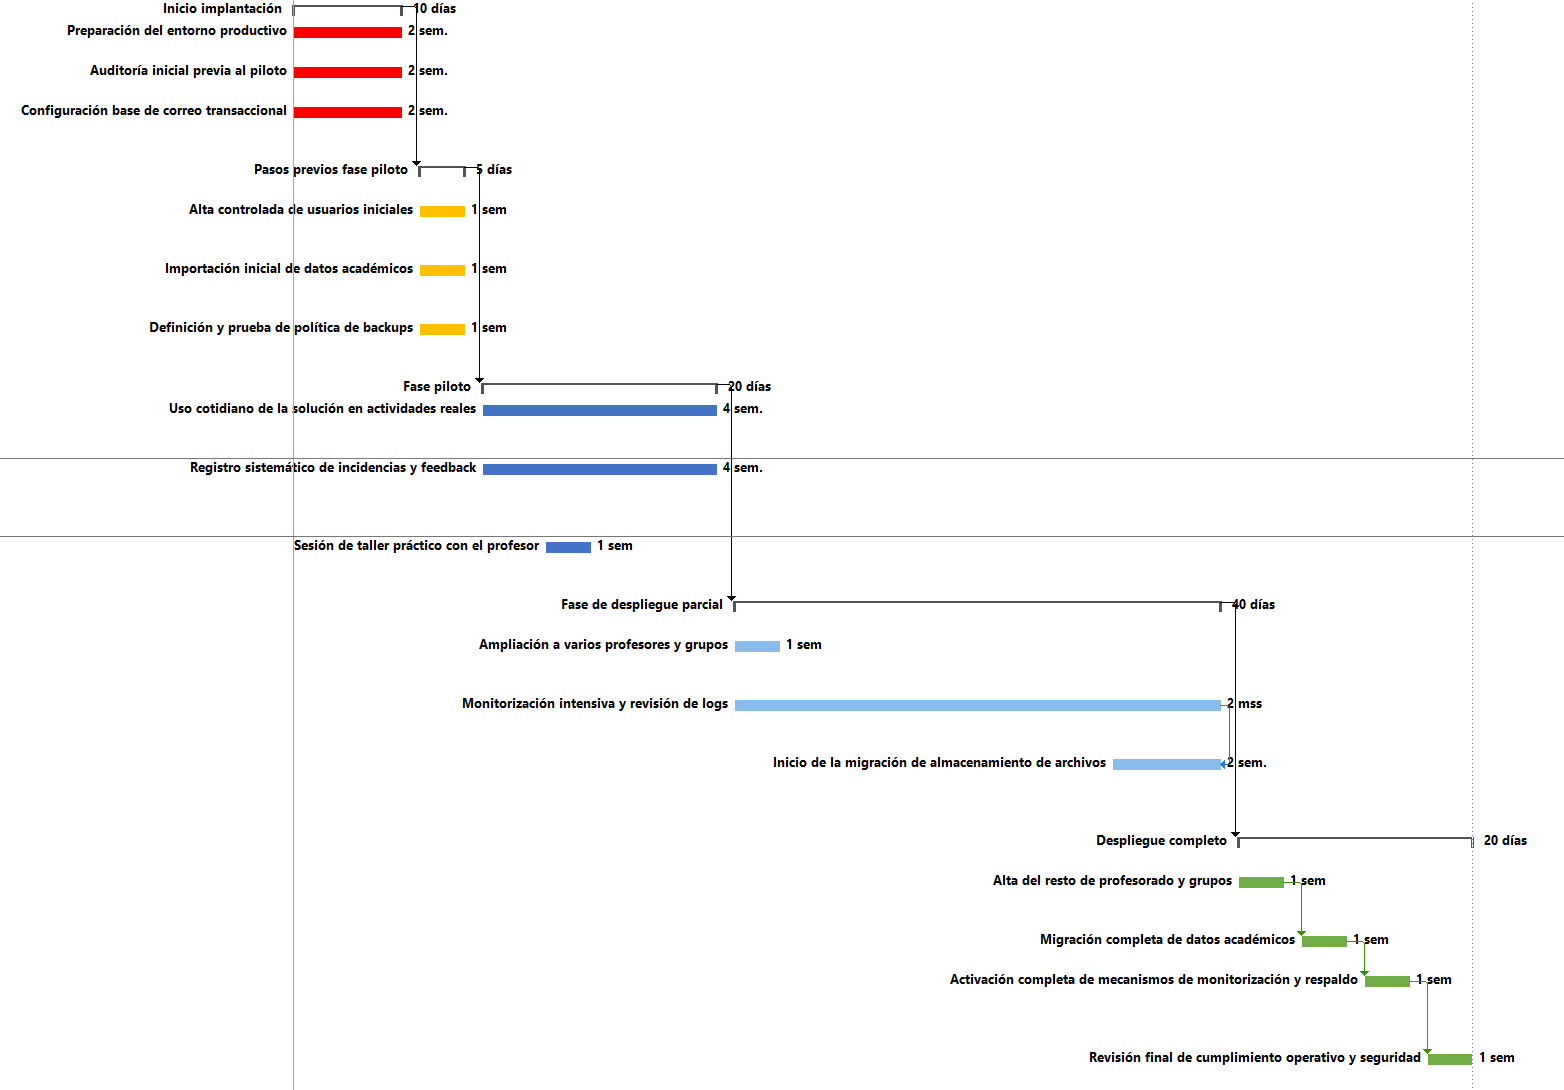
\includegraphics[width=\textwidth]{Figuras/cronogramaImplantacion.png}
  \caption{Cronograma orientativo de implantación}
  \label{fig:cronograma_implantacion}
\end{figure}

Este cronograma se concibe como un instrumento de control y toma de decisiones: cada fase finaliza con un hito de validación que determina si se avanza a la siguiente etapa o si se ejecuta una iteración correctiva. En este sentido, la validación práctica descrita en la sección~\ref{sec:validacion_preliminar} puede interpretarse como una evidencia empírica preliminar equivalente a una comprobación propia del piloto, aunque realizada fuera del marco formal completo, reforzando la utilidad de planificar la implantación con un enfoque incremental.

\section{Validación práctica en entorno educativo real}
\label{sec:validacion_preliminar}

Una vez definido el plan de implantación completo descrito en las secciones anteriores, se llevó a cabo una \textbf{validación práctica preliminar} del sistema en un entorno educativo real. Aunque esta experiencia no constituye una implantación formal siguiendo todas las fases del plan descrito, sí representa un \textbf{primer contacto real con usuarios finales}, aportando un elevado valor académico y permitiendo contrastar la idoneidad funcional, pedagógica y tecnológica de la solución desarrollada.

Esta validación se realizó mediante una sesión de demostración en un centro educativo con el que el autor del proyecto mantiene una vinculación directa como docente, lo que permitió desarrollar la experiencia en un entorno real, familiar y pedagógicamente representativo. Este contexto facilitó un intercambio cercano y sincero con profesorado y alumnado, aportando una perspectiva especialmente valiosa para la evaluación del sistema.

La sesión contó con la participación de una profesora de lenguaje musical y varios alumnos, con el objetivo de evaluar:

\begin{itemize}
    \item La facilidad de uso de la aplicación.
    \item La comprensión de la interfaz por parte del alumnado.
    \item La adecuación pedagógica de los flujos de trabajo.
    \item La utilidad real de las funcionalidades incorporadas en este complemento.
\end{itemize}

Asimismo, esta experiencia permitió detectar pequeños problemas de usabilidad y comportamiento visual que fueron corregidos posteriormente, reforzando la calidad final del sistema y evidenciando la importancia de una fase de validación empírica dentro del ciclo de vida del software educativo.

\subsection{Contexto de la demostración}

La demostración se realizó en la Escuela de Música Manuel Sánchez Alonso, perteneciente a la Asociación Cultural Musical Eladio Guzmán, en colaboración directa con el profesorado del centro y dentro de un contexto de enseñanza habitual del lenguaje musical.

Se presentó la aplicación tanto en su versión web como en su versión móvil Android, con el objetivo de mostrar:

\begin{itemize}
    \item La coherencia funcional entre plataformas.
    \item La correcta adaptación visual en dispositivos móviles.
    \item La utilidad real de las nuevas funcionalidades implementadas.
\end{itemize}

Durante la sesión, se expusieron las principales áreas de la aplicación: gestión de grupos, publicación de material, tareas, cuestionarios y el nuevo sistema de pistas inteligentes. Los alumnos interactuaron directamente con la plataforma, completando cuestionarios, consultando material y navegando por las distintas ramas de contenido, lo que permitió observar de forma directa su comportamiento y grado de adaptación.

\subsection{Valoración del profesorado}

La profesora participante, Patricia, docente de lenguaje musical en el centro, ofreció una valoración muy positiva del sistema, destacando especialmente su \textbf{carácter completo, atractivo e intuitivo}. En particular, subrayó los siguientes aspectos:

\begin{itemize}
    \item \textbf{Facilidad de uso:} La interfaz fue percibida como muy clara y sencilla, permitiendo un manejo natural sin necesidad de formación previa intensiva.
    \item \textbf{Centralización de recursos:} La posibilidad de disponer en un único entorno de materiales, tareas, calificaciones y comunicación fue considerada una mejora sustancial respecto a los métodos tradicionales empleados en el aula.
    \item \textbf{Facilidad de seguimiento:} El acceso inmediato al estado de entregas y calificaciones proporcionó una visión clara y estructurada del progreso del alumnado.
    \item \textbf{Utilidad del sistema de pistas:} Se valoró especialmente la incorporación de ayudas controladas durante la realización de cuestionarios, considerándolas un mecanismo pedagógicamente adecuado para reconducir el razonamiento del alumno sin ofrecer directamente la respuesta.
\end{itemize}

Asimismo, la docente destacó el \textbf{alto potencial de implantación real} de la herramienta en la dinámica habitual del aula, señalando que su uso podría mejorar notablemente la organización del trabajo, la comunicación con el alumnado y la motivación general durante el aprendizaje del lenguaje musical.

\subsection{Reacciones del alumnado}

El alumnado mostró una respuesta muy positiva ante el uso de la plataforma, destacando especialmente:

\begin{itemize}
    \item La claridad de la interfaz.
    \item La facilidad de navegación.
    \item El atractivo visual del entorno.
    \item La utilidad de las pistas durante los cuestionarios.
\end{itemize}

Durante la sesión, se observó un alto grado de implicación y curiosidad por parte de los alumnos, que se mostraron especialmente motivados al interactuar con los cuestionarios y los contenidos multimedia. La experiencia resultó llamativa para ellos, favoreciendo una participación activa y una actitud positiva hacia la actividad propuesta.

Además, se comprobó que comprendían rápidamente la lógica de funcionamiento de la aplicación, accedían sin dificultad a los contenidos y realizaban las entregas sin necesidad de explicaciones extensas, lo que refuerza la validez del diseño UX/UI descrito en la sección~\ref{sec:frontend_diseno_ext}.

\subsection{Problemas detectados y mejoras aplicadas}

La validación práctica permitió identificar una serie de pequeños problemas de diseño, usabilidad y comportamiento que no habían sido detectados durante las fases previas de desarrollo y pruebas en entorno controlado. Estos aspectos, aunque no comprometían el funcionamiento general del sistema, sí afectaban a la calidad de la experiencia de usuario y a la percepción de madurez de la aplicación.

Entre los principales puntos detectados se encuentran:

\begin{itemize}
    \item Ajustes de tamaño en ciertos elementos visuales en pantallas pequeñas.
    \item Pantalla de carga móvil no funcional.
    \item Ausencia de iconos representativos y feedback visual insuficiente ante situaciones de error.
    \item Formularios que no se limpiaban correctamente tras determinadas operaciones.
\end{itemize}

Estos problemas fueron abordados inmediatamente tras la sesión de validación, dando lugar a una \textbf{fase correctiva específica}, orientada a mejorar la estabilidad visual, la claridad de la interfaz y la calidad de la interacción con el usuario. Las correcciones se implementaron de forma iterativa, verificando su impacto directamente en dispositivos reales.

Este proceso pone de manifiesto la importancia de incorporar fases de validación empírica dentro del plan de implantación, ya que permite detectar fricciones reales en el uso cotidiano de la aplicación, imposibles de anticipar completamente durante el desarrollo teórico. Asimismo, evidencia el valor de la observación directa y del feedback inmediato como herramientas fundamentales para la mejora continua del sistema.

\subsection{Valor académico de la validación empírica}

La realización de esta demostración aporta un valor añadido significativo al proyecto desde un punto de vista académico:

\begin{itemize}
    \item Permite validar empíricamente las decisiones de diseño.
    \item Refuerza la orientación práctica del trabajo.
    \item Introduce colaboración externa real.
    \item Conecta el desarrollo técnico con su impacto pedagógico.
\end{itemize}

Además, esta experiencia permite afirmar que el sistema no solo es técnicamente viable, sino también funcionalmente adecuado y pedagógicamente coherente con los objetivos educativos planteados.

\begin{figure}[H]
  \centering
  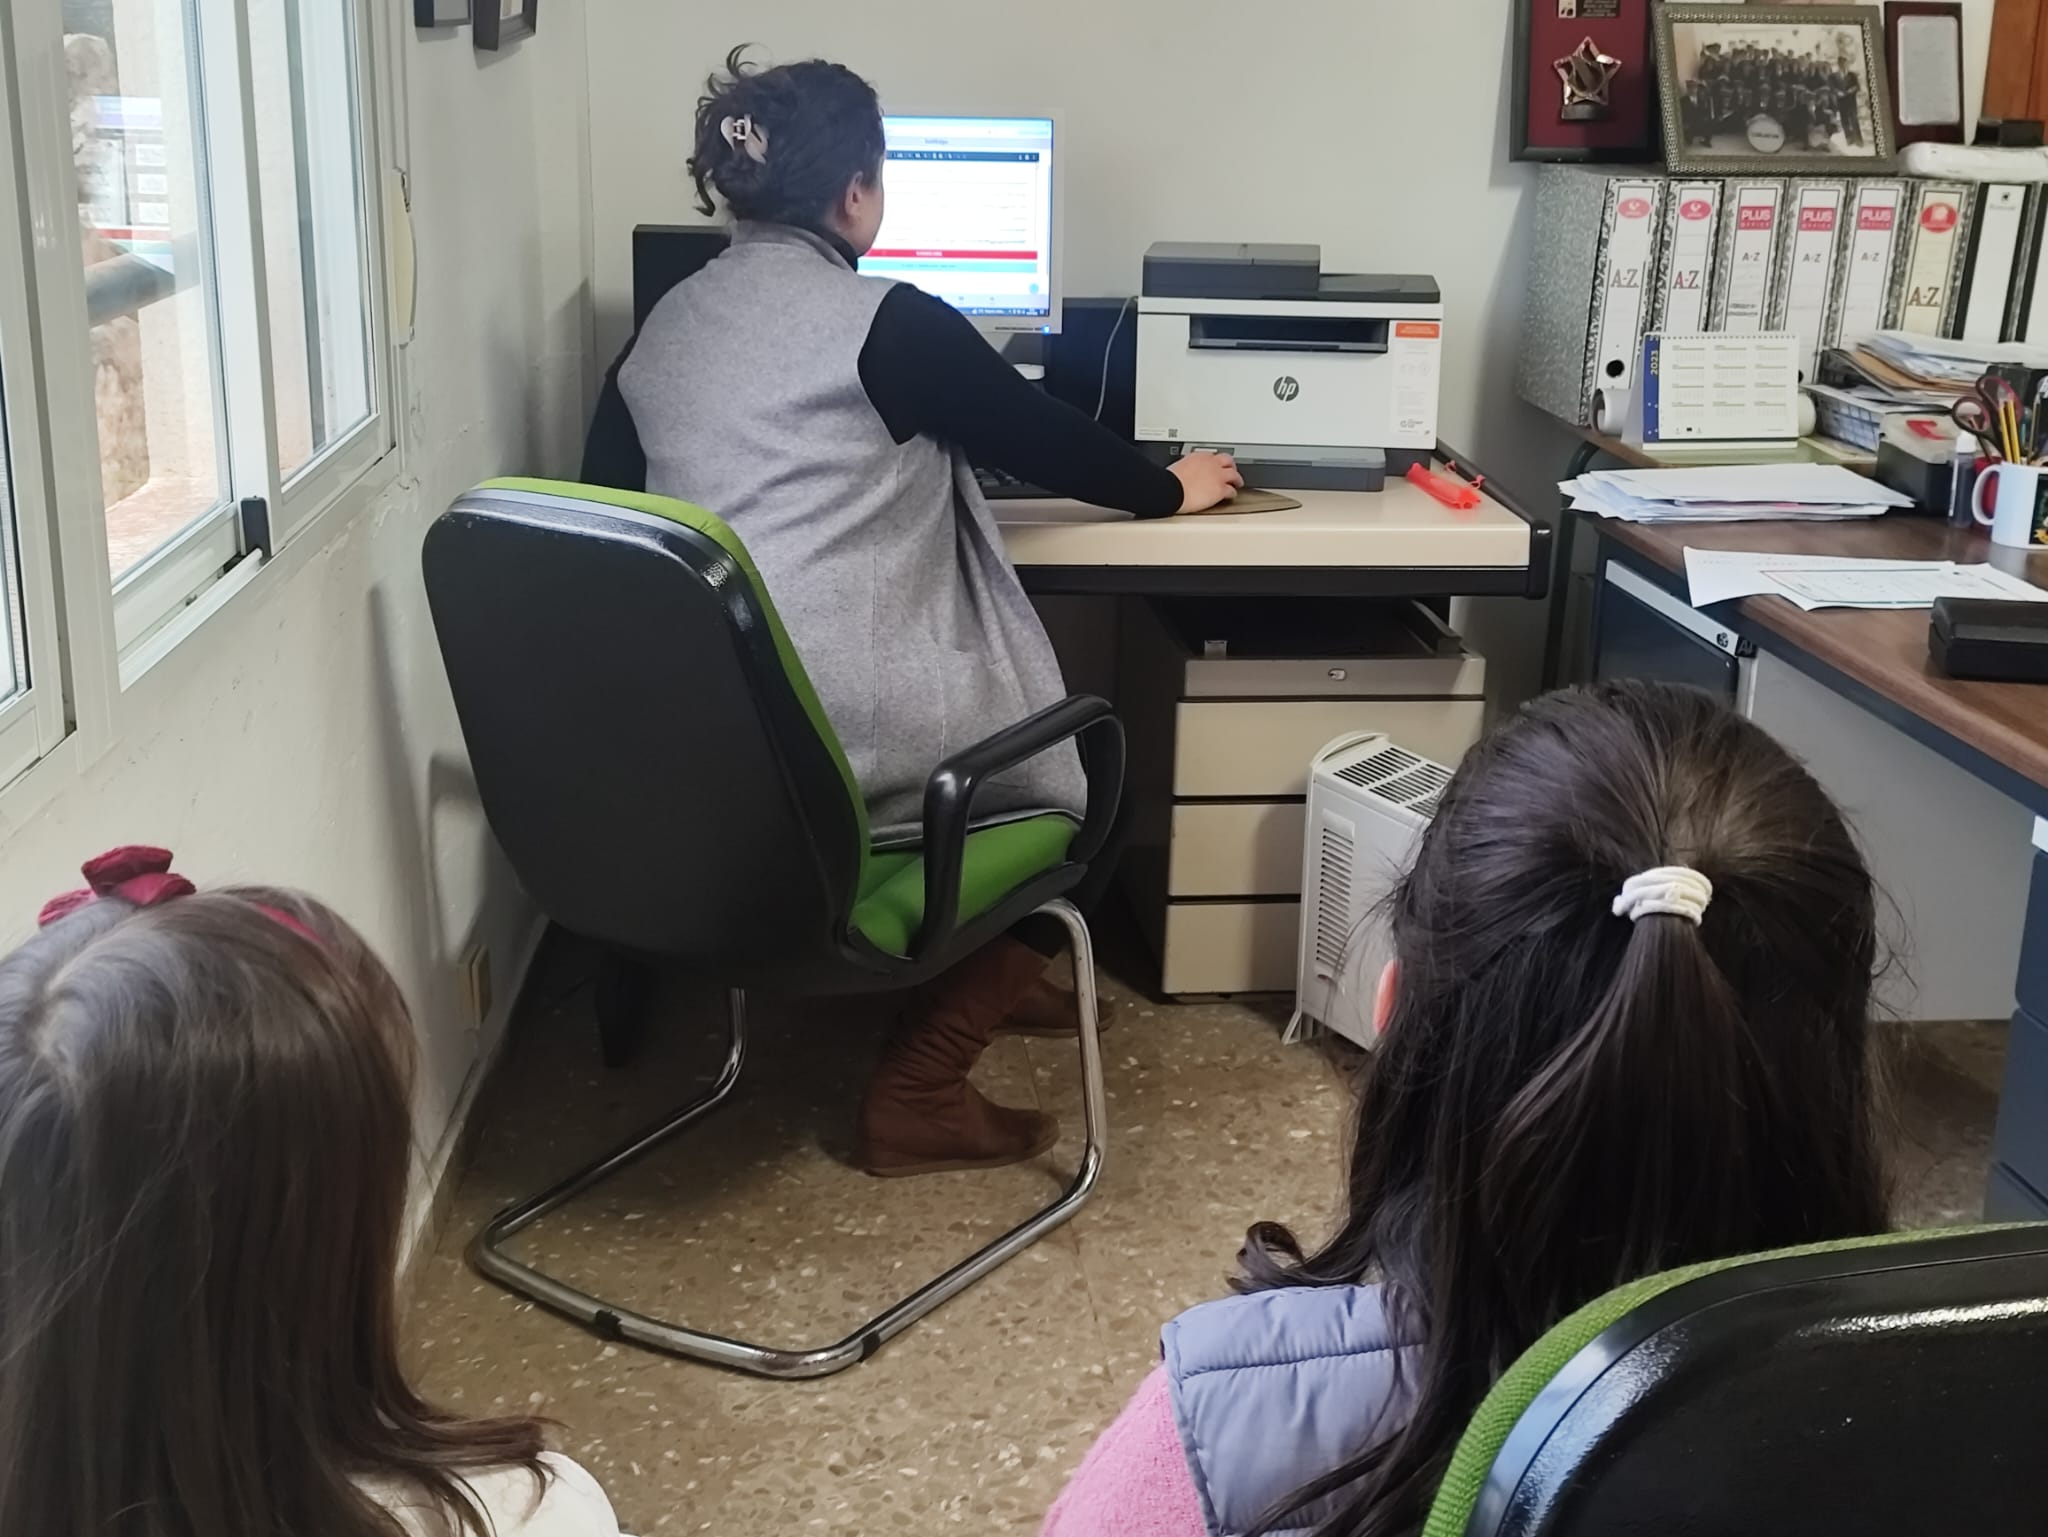
\includegraphics[width=0.48\textwidth]{Figuras/demostracion_aula_1.jpeg}\hfill
  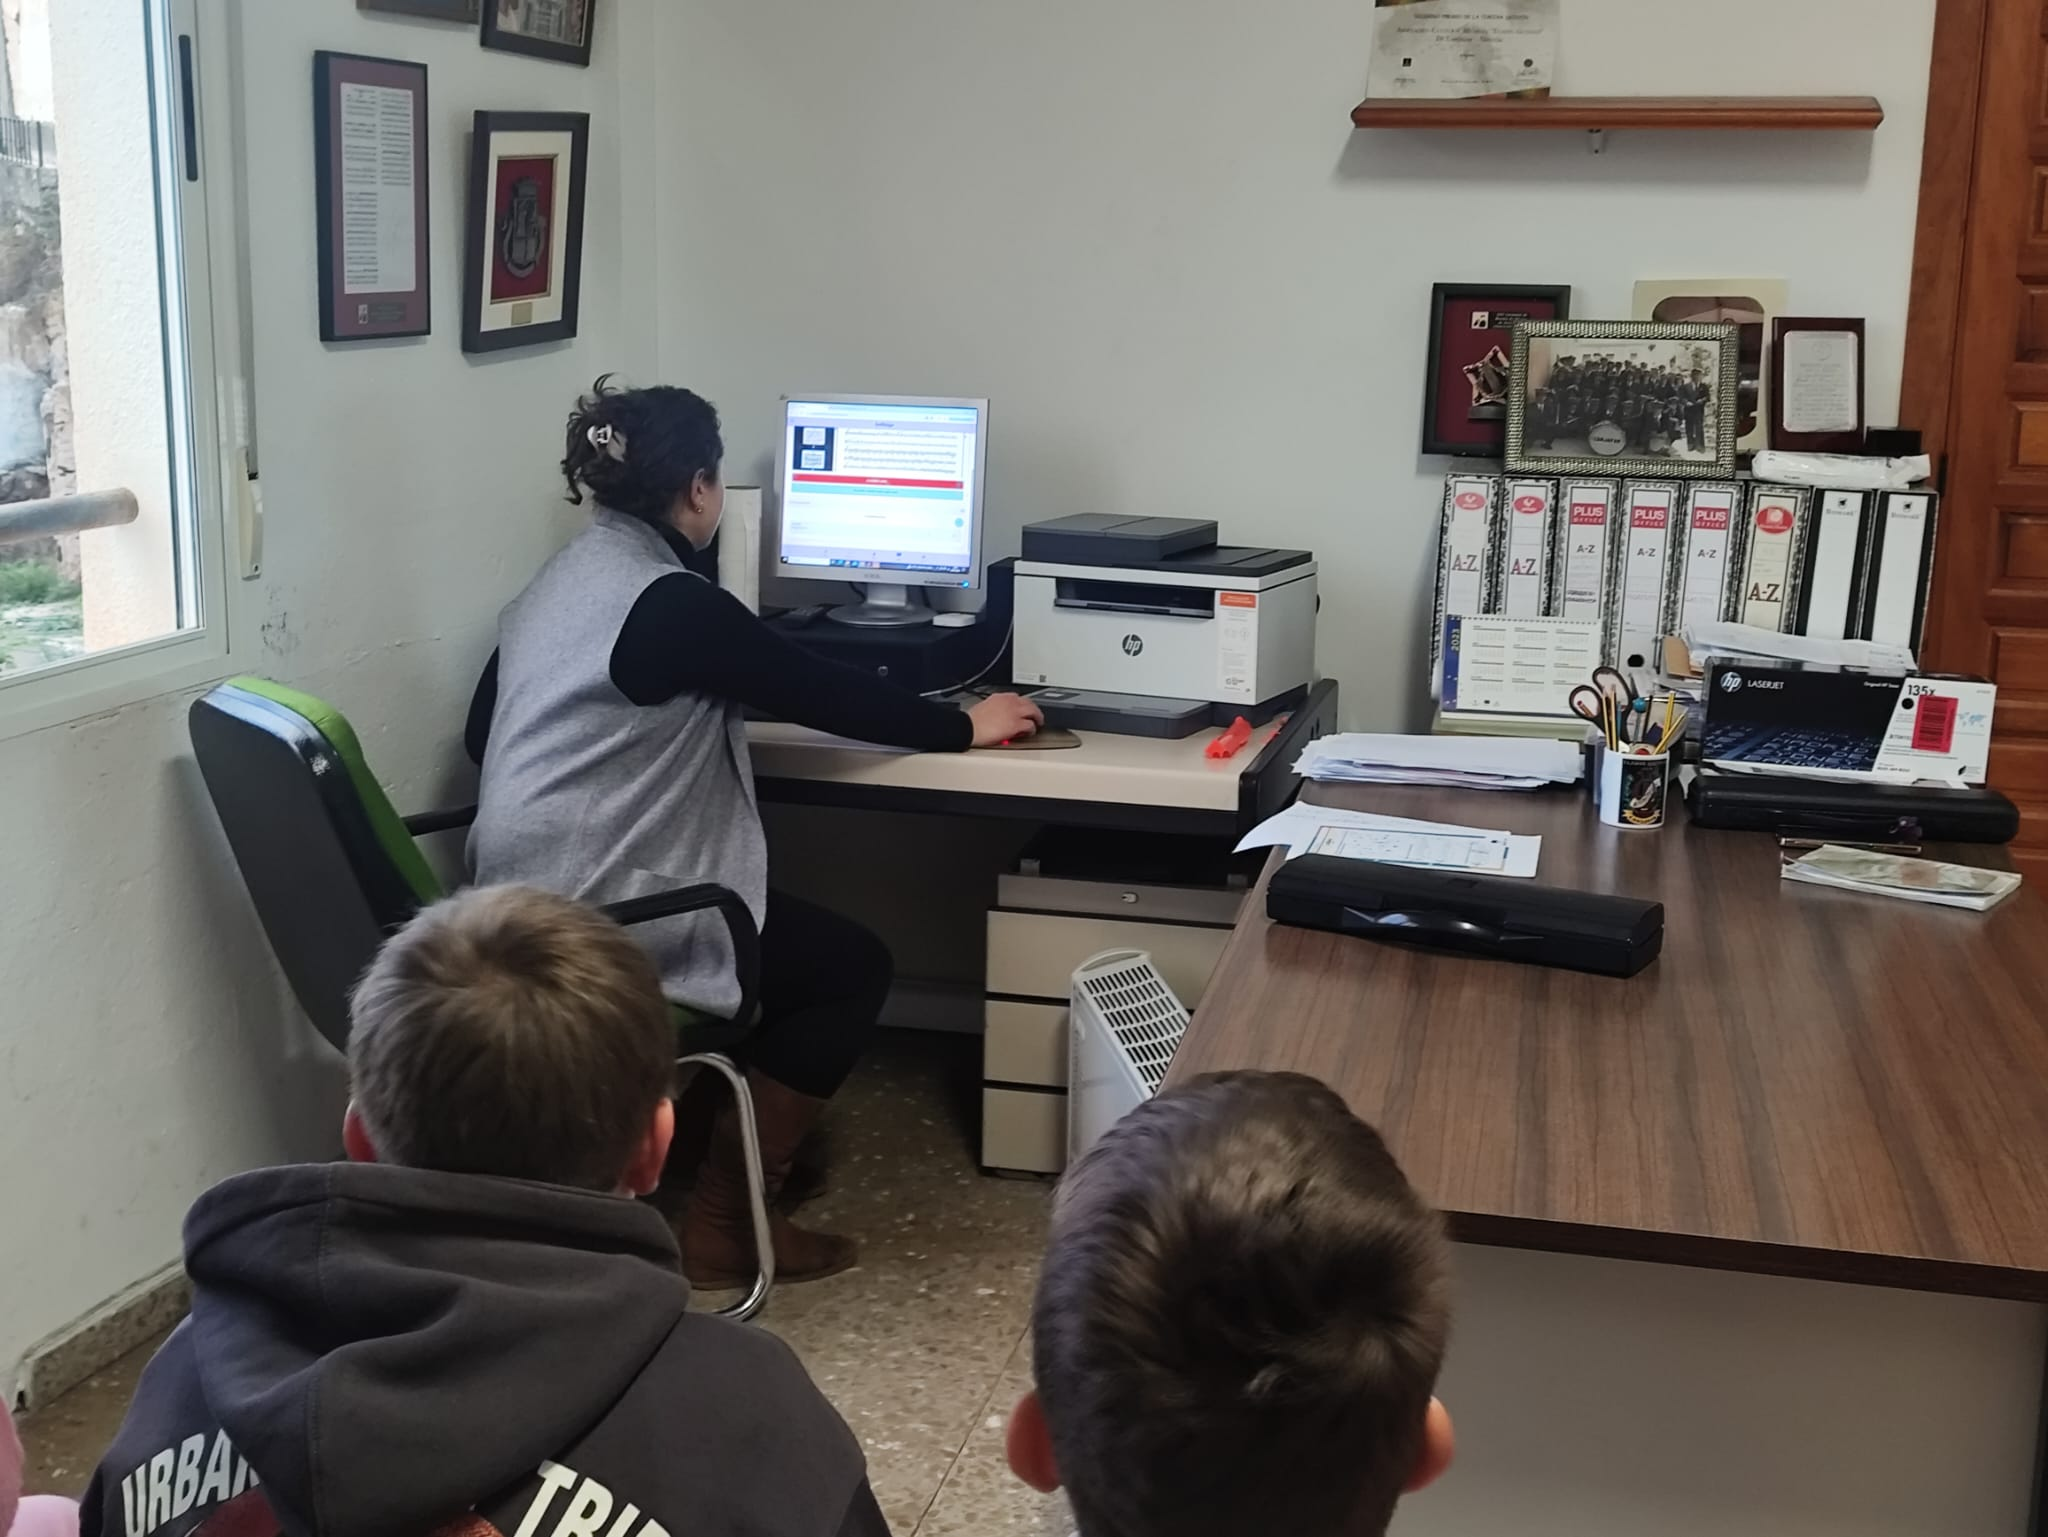
\includegraphics[width=0.48\textwidth]{Figuras/demostracion_aula_2.jpeg}
  \caption{Demostración de la aplicación en un entorno real de aula}
  \label{fig:demo_aula}
\end{figure}


\section{Síntesis del plan de implantación}
\label{sec:sintesis_implantacion}

El plan de implantación presentado establece una hoja de ruta completa para trasladar la solución desde un entorno académico hacia un contexto real de uso educativo. A través de una estrategia progresiva (sección~\ref{sec:estrategia_implantacion}), se asegura que la adopción del sistema se realice de forma controlada, permitiendo validar estabilidad, rendimiento y aceptación por parte de los usuarios antes de su despliegue completo.

Desde el punto de vista técnico, el plan define un proceso de migración hacia un entorno productivo apoyado en servicios escalables (sección~\ref{sec:migracion_tecnologica}), garantizando que el crecimiento del número de usuarios pueda abordarse sin reestructurar la arquitectura. Del mismo modo, se contempla la evolución de componentes críticos como el almacenamiento de ficheros (sección~\ref{sec:migracion_archivos}) y la profesionalización del correo electrónico (sección~\ref{sec:correo_profesional}), elementos clave para operar con fiabilidad en escenarios reales.

En paralelo, se integra la seguridad como un proceso operativo de supervisión y cumplimiento (sección~\ref{sec:seguridad_implantacion}), y se incorpora un plan de adopción orientado a minimizar fricciones en el uso cotidiano del sistema (sección~\ref{sec:formacion_implantacion}). Aunque el plan no se ha ejecutado en su totalidad durante el desarrollo del proyecto, la validación práctica preliminar realizada (sección~\ref{sec:validacion_preliminar}) aporta evidencia empírica y refuerza la utilidad de estructurar una implantación en fases.

En conjunto, este capítulo completa el ciclo de vida del proyecto más allá del desarrollo funcional descrito en el apartado \ref{sec:arquitectura_implementacion}, demostrando una visión integral de despliegue, operación y evolución. De este modo, la solución no se presenta únicamente como un prototipo académico, sino como una plataforma con un plan realista de implantación y un potencial de impacto educativo sostenible.

\chapter{Conclusiones y líneas de trabajo futuro}
\label{chap:conclusiones_complemento}

En este capítulo se presentan las conclusiones finales del proyecto de complemento, evaluando el grado de cumplimiento de los objetivos planteados y el valor añadido aportado respecto al proyecto original, así como una reflexión sobre las principales líneas de trabajo futuro que permitirían seguir ampliando, mejorando y consolidando la solución desarrollada.

\section{Conclusiones}

El objetivo general de este proyecto de complemento ha sido extender e implantar la solución informática desarrollada en el proyecto previo, llevándola a un nivel superior tanto en términos funcionales como de preparación para su uso en entornos educativos reales. A lo largo del desarrollo, este objetivo se ha abordado mediante la mejora progresiva de la aplicación, la incorporación de nuevas funcionalidades, la adaptación a entornos móviles y la definición de un plan de implantación estructurado y realista.

En relación con los subobjetivos definidos, se pueden extraer las siguientes conclusiones:

\begin{itemize}
    \item \textbf{Mejora y refinamiento de funcionalidades existentes:}  
    Se han optimizado diversos aspectos de la aplicación original, mejorando la estabilidad, la usabilidad y la claridad de la interfaz. Estas mejoras han permitido adaptar la solución a flujos de trabajo reales, reforzando su adecuación al contexto educativo y aumentando la calidad de la experiencia de usuario tanto para profesorado como para alumnado.

    \item \textbf{Incorporación de nuevas funcionalidades innovadoras:}  
    El proyecto ha ampliado significativamente el alcance funcional de la plataforma, integrando nuevos mecanismos orientados a enriquecer el proceso de aprendizaje y a reforzar el valor pedagógico de la herramienta. Estas incorporaciones aportan un carácter innovador al sistema y permiten explorar nuevas metodologías educativas apoyadas en tecnología.

    \item \textbf{Adaptación y despliegue en entornos móviles:}  
    Gracias al uso de una arquitectura híbrida y diseño responsive, se ha logrado generar una versión móvil plenamente funcional de la aplicación, garantizando una experiencia de usuario coherente en dispositivos Android. Esta extensión incrementa notablemente la accesibilidad, portabilidad y flexibilidad del sistema, facilitando su integración en la dinámica educativa diaria.
\newpage
    \item \textbf{Definición de un plan de implantación realista:}  
    Se ha elaborado un plan de implantación integral que abarca aspectos técnicos, organizativos, de seguridad y formativos, estableciendo una hoja de ruta clara para el despliegue progresivo del sistema en centros educativos reales. Este plan permite transformar un desarrollo académico en una solución con viabilidad operativa, aportando una visión profesional del ciclo de vida del software.
\end{itemize}

Adicionalmente, la realización de una validación práctica en un entorno educativo real ha permitido contrastar empíricamente la idoneidad funcional, pedagógica y tecnológica del sistema, reforzando la calidad final de la solución y evidenciando la importancia de incorporar procesos de evaluación con usuarios finales.

En conjunto, el proyecto de complemento ha permitido consolidar la plataforma desarrollada, dotándola de una mayor madurez técnica, una funcionalidad ampliada y una proyección realista hacia su implantación en entornos educativos reales, cerrando así de forma coherente el ciclo completo de análisis, desarrollo, validación e implantación.

\section{Líneas de trabajo futuro}

A pesar de los avances alcanzados, el sistema mantiene un amplio margen de crecimiento. La propia evolución del complemento ha puesto de manifiesto nuevas necesidades y oportunidades de mejora que configuran un conjunto rico de líneas de trabajo futuro.

\subsection{Ejecución completa del plan de implantación en un centro educativo}

Aunque se ha definido un plan de implantación detallado y se ha realizado una validación preliminar, una de las principales líneas futuras consiste en la \textbf{ejecución completa del despliegue en un centro educativo real}, siguiendo todas las fases propuestas.

Este trabajo permitiría:
\begin{itemize}
    \item Validar el comportamiento del sistema en uso continuado.
    \item Analizar métricas reales de carga, rendimiento y estabilidad.
    \item Obtener retroalimentación prolongada del profesorado y alumnado.
    \item Ajustar procesos organizativos y técnicos en función del uso real.
\end{itemize}

La implantación completa consolidaría la madurez del sistema y permitiría evaluar su impacto pedagógico de forma longitudinal.
\newpage
\subsection{Extensión continua de funcionalidades e innovación pedagógica}

El complemento ha incorporado mejoras relevantes, pero la naturaleza del dominio educativo permite una evolución funcional constante. Entre las posibles extensiones futuras destacan:

\begin{itemize}
    \item Evolución del sistema de ayudas inteligentes mediante mayor personalización, adaptación al progreso del alumno y análisis de errores recurrentes.
    \item Incorporación de nuevos módulos didácticos interactivos (entrenamiento auditivo, dictados rítmicos, reconocimiento melódico, etc.).
    \item Desarrollo de herramientas de analítica educativa que faciliten el seguimiento del progreso y la toma de decisiones pedagógicas.
\end{itemize}

Estas ampliaciones reforzarían el valor diferencial de la plataforma y su alineación con metodologías educativas activas.

\subsection{Apertura del sistema a usuarios externos y acceso sin autenticación}

Tal como se planteaba en el proyecto original, permanece pendiente la apertura parcial del sistema a usuarios no autenticados o no vinculados a centros educativos. Esta línea permitiría:

\begin{itemize}
    \item Facilitar el acceso a contenidos demostrativos.
    \item Permitir el registro de usuarios independientes.
    \item Aumentar la difusión y visibilidad del proyecto.
\end{itemize}

La implementación de este modelo requeriría un diseño cuidadoso de permisos, privacidad y segmentación funcional.

\subsection{Tecnologías de mantenimiento, monitorización y gestión de logs}

La evolución del sistema hacia escenarios productivos introduce la necesidad de reforzar las capacidades de mantenimiento y supervisión. Como líneas futuras se plantea:

\begin{itemize}
    \item Integración de sistemas de logging estructurado.
    \item Centralización de registros y trazabilidad de eventos.
    \item Incorporación de monitorización, métricas y alertas automáticas.
\end{itemize}

Estas mejoras permitirían detectar incidencias de forma temprana, reducir tiempos de resolución y aumentar la estabilidad operativa del sistema.

\subsection{Refuerzo de la seguridad y mejora en la gestión de credenciales}

La seguridad emerge como una línea prioritaria de evolución. Entre las mejoras futuras destacan:

\begin{itemize}
    \item Sustitución del envío directo de credenciales por flujos seguros basados en enlaces de activación y restablecimiento de contraseña.
    \item Gestión avanzada de secretos mediante servicios dedicados.
    \item Implementación de políticas de autenticación reforzada y control de accesos.
\end{itemize}

Estas acciones permitirían elevar significativamente el nivel de protección de datos personales, especialmente relevante en contextos educativos con menores.

En conclusión, el proyecto de complemento no solo ha permitido materializar líneas de evolución previamente planteadas, sino que ha abierto nuevas vías de mejora orientadas a la profesionalización, la seguridad y la sostenibilidad del sistema. De este modo, la solución desarrollada se consolida como una plataforma con un alto potencial de crecimiento, capaz de adaptarse progresivamente a las exigencias técnicas, pedagógicas y organizativas de un entorno educativo real.


\bibliography{referencias}
%\clearpage



\clearpage
\backmatter

\thispagestyle{empty}
%\put(0,0){
\begin{minipage}[h]{0.9\paperwidth}
\thispagestyle{empty}
\begin{tikzpicture}[remember picture,overlay]
\node (f) [rectangle]  
at (current page.center)
          {\parbox[b][\paperheight]{\paperwidth}{
           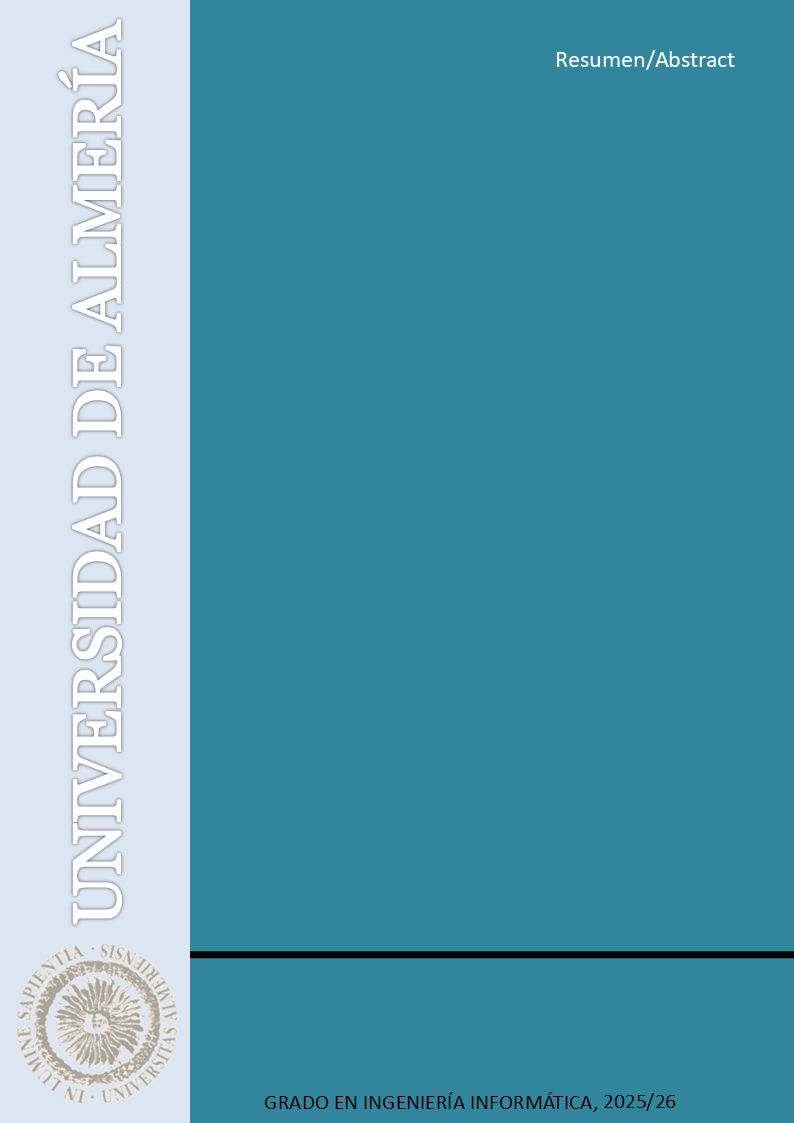
\includegraphics[width=\paperwidth,height=\paperheight,keepaspectratio]{Figuras/logos/contraportadaCTFG.png}
          }};
\node (texto) [rectangle,text width=0.5\paperwidth,yshift=150pt] 
at (f)
          {\parbox{0.65\paperwidth}{\justifying \Large \color{white}
         El complemento del proyecto ha consistido en la ampliación y evolución técnica de la solución informática desarrollada previamente, abordando aspectos avanzados como la arquitectura cloud, el despliegue móvil, la integración de inteligencia artificial y la definición de un plan de implantación orientado a su aplicación en entornos educativos reales.

\vspace{1.5cm}

%\section*{Abstract}
The complementary part of the project has consisted of the technical extension and evolution of the previously developed software solution, addressing advanced aspects such as cloud architecture, mobile deployment, artificial intelligence integration, and the definition of a deployment plan aimed at its application in real educational environments.

         }};
  \end{tikzpicture}
\end{minipage}
%}


          
          

\end{document}
